\documentclass[10pt, letterpaper]{article}

% Inhaltsverzeichnis für Pakettypen (nur für Übersicht im Header, wird nicht im Dokument angezeigt)
% 1. Seitenlayout und Ränder
% 2. Sprache und Zeichensatz
% 3. Mathematik und Theorem-Umgebungen
% 4. Eigene Makros
% 5. Diagramme und Grafiken
% 6. Tabellen und Aufzählungen
% 7. Inhaltsverzeichnis
% 8. Abschnittsüberschriften
% 9. Abstrakt-Umgebung
% 10. Todos/Notizen
% 11. Rahmen/Box-Umgebungen
% 12. Python-Integration
% 13. Literaturverwaltung
% 14. Hyperlinks
% 15. Absatzeinstellungen
% 16. Umgebungen
% 17  Graphik
% 00. Titel und Autor

% --- 1. Seitenlayout und Ränder ---
\usepackage[margin=3cm]{geometry}

% --- 2. Sprache und Zeichensatz ---
\usepackage[english]{babel}
\usepackage[T1]{fontenc}
\usepackage[utf8]{inputenc}

% --- 3. Mathematik und Theorem-Umgebungen ---
\usepackage{amsmath, amssymb, amsthm}
\usepackage{mathrsfs}
\DeclareMathOperator{\WF}{WF}

% --- 4. Eigene Makros ---
\usepackage{xcolor}
\newcommand{\SKP}{\langle\cdot,\cdot\rangle}
\newcommand{\R}{\mathbb{R}}
\newcommand{\N}{\mathbb{N}}
\newcommand{\Q}{\mathbb{Q}}
\newcommand{\Z}{\mathbb{Z}}
\newcommand{\C}{\mathbb{C}}
\newcommand{\entwurf}[1]{\textcolor{red}{#1}}

% --- 5. Diagramme und Grafiken ---
\usepackage{graphicx}
\usepackage{tikz}
\usetikzlibrary{decorations.pathreplacing, arrows.meta, positioning}
\usepackage{tikz-cd}

% --- 6. Tabellen und Aufzählungen ---
\usepackage{enumitem}
\setlist[itemize]{left=0.5cm}

\newenvironment{romanenum}[1][]
  {%
    \ifx&#1&
    \else
      \textbf{#1}\quad
    \fi
    \begin{enumerate}[label=\roman*)]
  }
  {%
    \end{enumerate}%
  }

% --- 7. Inhaltsverzeichnis ---
\usepackage{tocloft}
\renewcommand{\cftsecfont}{\footnotesize}
\renewcommand{\cftsubsecfont}{\footnotesize}
\renewcommand{\cftsubsubsecfont}{\footnotesize}
\renewcommand{\cftsecpagefont}{\footnotesize}
\renewcommand{\cftsubsecpagefont}{\footnotesize}
\renewcommand{\cftsubsubsecpagefont}{\footnotesize}
\usepackage{etoc}

% --- 8. Abschnittsüberschriften ---
\usepackage{titlesec}
\titleformat{\section}{\normalfont\large\bfseries}{\thesection}{1em}{}
\titleformat{\subsection}{\normalfont\normalsize\bfseries}{\thesubsection}{0.5em}{}
\titleformat{\subsubsection}{\normalfont\normalsize\bfseries}{\thesubsubsection}{0.5em}{}
\setcounter{secnumdepth}{4}

% --- 9. Abstrakt-Umgebung ---
\usepackage{changepage}
\renewenvironment{abstract}
  {
    \begin{adjustwidth}{1.5cm}{1.5cm}
    \small
    \textsc{Abstract. –}%
  }
  {
    \end{adjustwidth}
  }

% --- 10. Todos/Notizen ---
\usepackage{todonotes}

% --- 11. Rahmen/Box-Umgebungen ---
\usepackage{mdframed}
\usepackage{tcolorbox}
\colorlet{shadecolor}{gray!25}

\newenvironment{customTheorem}
  {\vspace{10pt}%
   \begin{mdframed}[
     backgroundcolor=gray!20,
     linewidth=0pt,
     innertopmargin=10pt,
     innerbottommargin=10pt,
     skipabove=\dimexpr\topsep+\ht\strutbox\relax,
     skipbelow=\topsep,
   ]}
  {\end{mdframed}
   \vspace{10pt}%
  }

% --- 12. Python-Integration ---
% (Deaktiviert in dieser Version, aktiviere bei Bedarf)
% \usepackage{pythontex}
% \usepackage[makestderr]{pythontex}

% --- 13. Literaturverwaltung ---
\usepackage{csquotes}
\usepackage[backend=biber, style=alphabetic, citestyle=alphabetic]{biblatex}
\addbibresource{bibliography.bib}

% --- 14. Hyperlinks ---
\usepackage{hyperref}
\hypersetup{
  colorlinks   = true,
  urlcolor     = blue,
  linkcolor    = blue,
  citecolor    = blue,
  frenchlinks  = true
}

% --- 15. Absatzeinstellungen ---
\usepackage[parfill]{parskip}
\sloppy

% --- 16. Umgebungen ---
\usepackage{thmtools}

\newcommand{\CustomHeading}[3]{%
  \par\medskip\noindent%
  \textbf{#1 #2} \textnormal{(#3)}.\enskip%
}

\newenvironment{DEF}[2]{\begin{unitbox}\CustomHeading{Definition}{#1}{#2}}{\end{unitbox}}
\newenvironment{PROP}[2]{\begin{unitbox}\CustomHeading{Proposition}{#1}{#2}}{\end{unitbox}}
\newenvironment{THEO}[2]{\begin{unitbox}\CustomHeading{Theorem}{#1}{#2}}{\end{unitbox}}
\newenvironment{LEM}[2]{\begin{unitbox}\CustomHeading{Lemma}{#1}{#2}}{\end{unitbox}}
\newenvironment{KORO}[2]{\begin{unitbox}\CustomHeading{Corollar}{#1}{#2}}{\end{unitbox}}
\newenvironment{REM}[2]{\begin{unitbox}\CustomHeading{Remark}{#1}{#2}}{\end{unitbox}}
\newenvironment{EXA}[2]{\begin{unitbox}\CustomHeading{Example}{#1}{#2}}{\end{unitbox}}
\newenvironment{STUD}[2]{\begin{unitbox}\CustomHeading{Study}{#1}{#2}}{\end{unitbox}}
\newenvironment{CONC}[2]{\begin{unitbox}\CustomHeading{Concept}{#1}{#2}}{\end{unitbox}}
\newenvironment{OTH}[2]{\begin{unitbox}\CustomHeading{Other}{#1}{#2}}{\end{unitbox}}
\newenvironment{EXE}[2]{\begin{unitbox}\CustomHeading{Exercise}{#1}{#2}}{\end{unitbox}}
\newenvironment{MOT}[2]{\begin{unitbox}\CustomHeading{Motivation}{#1}{#2}}{\end{unitbox}}
\newenvironment{PROOF}[2]{\begin{unitbox}\CustomHeading{Proof}{#1}{#2}}{\end{unitbox}}

% --- Unit Umgebung für Source-Inhalte ---
\usepackage{mdframed}
\newmdenv[
  linewidth=1pt,
  topline=false,
  bottomline=false,
  rightline=false,
  leftmargin=0cm,
  rightmargin=0cm,
  skipabove=10pt,
  skipbelow=10pt,
  innertopmargin=0.5\baselineskip,
  innerbottommargin=0.5\baselineskip,
  backgroundcolor=gray!10,
  linecolor=gray
]{unitbox}

\newenvironment{unit}[1]
  {\begin{unitbox}\textbf{Unit #1}\par\smallskip}
  {\end{unitbox}}

% --- 17. Graphik ---
\usepackage{graphicx}
\graphicspath{ {./images/} }
\usepackage[export]{adjustbox}

% --- 00. Titel und Autor ---
\title{Mein Titel}
\author{Tim Jaschik}
\date{\today}

\begin{document}

\maketitle
\rule{\textwidth}{0.5pt}
\begin{abstract}
Kurze Beschreibung …
\end{abstract}
\rule{\textwidth}{0.5pt}
\vspace{0.5cm}

\tableofcontents

\pagebreak


\section*{KAPITEL 1}
\section*{Differenzierbare Mannigfaltigkeiten}
\section*{1. Untermannigfaltigkeiten in Euklidischen Räumen}
Definition 1.1. 

Eine Teilmenge $M \subset \mathbb{R}^{N}$ heisst $n$-dimensionale Untermannigfaltigkeit, falls es zu jedem Punkt $p \in M$ eine Umgebung $U \subset \mathbb{R}^{N}$ und einen Diffeomorphismus $f: U \rightarrow V \subset \mathbb{R}^{N}$ gibt so dass
$$
U \cap M=f^{-1}\left(V \cap \mathbb{R}^{n}\right) .
$$
Die Dimension von $M$ ist $n$, die Kodimension ist $N-n$. Untermannigfaltigkeiten der Dimension 2 heissen Flächen, Untermannigfaltigkeiten der Kodimension 1 heissen Hyperflächen.



BEISPIEL\\
(1) 


Die $n$-Sphäre
$$
S^{n}=\left\{x \in \mathbb{R}^{n+1} \mid x_{0}^{2}+\ldots+x_{n}^{2}=1\right\}
$$
ist eine $n$-dimensionale Untermannigfaltigkeit.


(2)

$$
H_{c}^{n}=\left\{x \in \mathbb{R}^{n+1} \mid x_{0}^{2}-x_{1}^{2}-x_{2}^{2}-\ldots-x_{n}^{2}-c=0\right\}
$$
ist für $c<0$ der einschalige Hyperboloid; für $c>0$ der zweischalige Hyperboloid; und für $c=0$ keine Untermannigfaltigkeit (Singularität im Punkt $(0, \ldots, 0)$ ).


(3) 



\begin{EXA}{RG-B25-02-04}{n-Torus}
Der $n$-Torus
$$
\begin{aligned}
T^{n} & =\left\{z \in \mathbb{C}^{n}| | z_{1}\left|=\ldots=\left|z_{n}\right|=1\right\}\right.
& =\left\{x \in \mathbb{R}^{2 n} \mid x_{1}^{2}+x_{2}^{2}-1=\ldots=x_{2 n-1}^{2}+x_{2 n}^{2}-1=0\right\}
\end{aligned}
$$
ist eine $n$-dimensionale Untermannigfaltigkeit in $\mathbb{R}^{2 n}$.
\end{EXA}



(4)

\begin{EXA}{RG-B25-02-05}{$SO(n)$}
$$
S O(n)=\left\{A \in M(n, n, \mathbb{R}) \mid A^{t} A=I d, \operatorname{det} A=1\right\}
$$
ist eine $\binom{n}{2}$-dimensionale Untermannigfaltigkeit in $M(n, n, \mathbb{R})=$ $\mathbb{R}^{n^{2}}$.
\end{EXA}



Satz 1.2. 

\begin{PROP}{RG-B25-02-06}{Charakterisierungen von Untermannigfaltigkeiten im euklidischen Raum}
Die folgenden Aussagen sind äquivalent:
\begin{enumerate}
    \item $M$ ist eine $n$-dimensionale Untermannigfaltigkeit in $\mathbb{R}^{N}$.
    
    \item Für jedes $p \in M$ gibt es eine Umgebung $U \subset \mathbb{R}^{N}$ und eine Submersion $f: U \rightarrow \mathbb{R}^{N-n}$ mit
    \[
    U \cap M = f^{-1}(0).
    \]

    \item Für jedes $p \in M$ gibt es eine Umgebung $V$ von $p$ in $\mathbb{R}^{N}$, eine offene Menge $U \subset \mathbb{R}^{n}$ und eine Abbildung $\psi \in C^{1}\left(U, \mathbb{R}^{N}\right)$ mit folgenden Eigenschaften:
    \begin{itemize}
        \item $\psi$ ist ein Homöomorphismus von $U$ auf $M \cap V$,
        \item $\psi^{-1}: M \cap V \rightarrow U$ ist stetig,
        \item $\left.d\psi\right|_{x}: \mathbb{R}^{n} \rightarrow \mathbb{R}^{N}$ ist injektiv für alle $x \in U$.
    \end{itemize}
\end{enumerate}
\end{PROP}


Bemerkung: in (2) bedeutet Submersion, dass $\left.d f\right|_{x}: T_{x} U=\mathbb{R}^{N} \rightarrow$ $T_{f(x)} \mathbb{R}^{N-n}=\mathbb{R}^{N-n}$ surjektiv ist für alle $x \in U$.

In Beispiel (1) kann man $f(x)=x_{0}^{2}+\ldots+x_{n}^{2}-1$ wählen. Dann ist $\left.d f\right|_{x}=2\left(x_{0}, \ldots, x_{n}\right)$. Ist $U:=\mathbb{R}^{n+1} \backslash\{0\}$, so ist $\left.d f\right|_{x}$ für alle $x \in U$ surjektiv. In Beispiel (2) wählt man $f(x)=x_{0}^{2}-x_{1}^{2}-x_{2}^{2}-\ldots-x_{n}^{2}-c$, in Beispiel (3) $f(x)=\left(x_{1}^{2}+x_{2}^{2}-1, \ldots, x_{2 n-1}^{2}+x_{2 n}^{2}-1\right)$. Beispiel (4) ist ÜA.

\section*{2. Glatte Mannigfaltigkeiten}

Definition 2.1. 

\begin{DEF}{RG-B25-03-01}{Atlas auf topologischen Hausdorff-Räumen}
Sei M ein topologischer Raum. Wir setzen voraus, dass $M$ Hausdorff ist, d.h. zu $p, q \in M, p \neq q$ existieren disjunkte offene Umgebungen. Weiterhin soll es eine abzählbare Basis der Topologie geben. Ein Atlas auf $M$ ist gegeben durch
\begin{enumerate}
  \item Eine offene Überdeckung $\left\{U_{i}\right\}_{i \in I}$ von $M$.
  \item Eine Familie von Karten $\phi_{i}: U_{i} \rightarrow W_{i} \subset \mathbb{R}^{n}$, die Homöomorphismen sind und die Eigenschaft haben, dass
  $$
  \phi_{j} \circ \phi_{i}^{-1}: \phi_{i}\left(U_{i} \cap U_{j}\right) \rightarrow \phi_{j}\left(U_{i} \cap U_{j}\right)
  $$
  Diffeomorphismen sind.
\end{enumerate}
\end{DEF}



Definition 2.2. 

\begin{DEF}{RG-B25-03-02}{Äquivalente Atlanten}
Zwei Atlanten $\left\{\left(U_{i}, \phi_{i}\right)\right\},\left\{\left(V_{j}, \psi_{j}\right)\right\}$ heissen äquivalent, wenn ihre Vereinigung wieder ein Atlas ist.
\end{DEF}

Achtung: Es gibt Atlanten, die nicht äquivalent sind, z.B. auf der 7-dimensionalen Sphäre (exotische Sphären).

DEFINITION 2.3. 


\begin{DEF}{RG-B25-03-04}{Glatte Mannigfaltigkeit}
Eine glatte Struktur auf einem Hausdorffschen topologischen Raum ist eine Äquivalenzklasse von Atlanten. M, zusammen mit einer glatten Struktur, heisst glatte Mannigfaltigkeit.
\end{DEF}



Bemerkung: 

\begin{DEF}{RG-B25-03-05}{Orientierte Mannigfaltigkeiten}
Setzt man in der Definition eines Atlanten zusätzlich voraus, dass die Abbildungen $\phi_{j} \circ \phi_{i}^{-1}: \phi_{i}\left(U_{i} \cap U_{j}\right) \rightarrow \phi_{j}\left(U_{i} \cap U_{j}\right)$ orientierungserhaltende Diffeomorphismen sind (d.h. positive Jacobideterminante haben), so spricht man von einer orientierten Mannigfaltigkeit.
\end{DEF}

Definition 2.4. 


\begin{DEF}{RG-B25-03-06}{Untermannigfaltigkeit einer Mannigfaltigkeit}
Eine Teilmenge $M$ einer Mannigfaltigkeit $N$ heisst Untermannigfaltigkeit falls es zu jedem $p \in M$ eine Karte ( $U, \phi$ ) von $N$ gibt mit $p \in U$ und so dass $\phi(U \cap M)$ eine Untermannigfaltigkeit von $\phi(U) \subset \mathbb{R}^{n}$ ist.
\end{DEF}



\section*{BEISPIEL}
(1) 


\begin{EXA}{RG-B25-03-07}{n-Torus als Mfk}
Torus
$$
T^{n}=\left\{z \in \mathbb{C}^{n}| | z_{1}\left|=\ldots=\left|z_{n}\right|=1\right\}\right.
$$
Definiere $f: \mathbb{R}^{n} \rightarrow \mathbb{C}^{n},\left(x_{1}, \ldots, x_{n}\right) \mapsto\left(e^{i x_{1}}, \ldots, e^{i x_{n}}\right)$. Dann ist $f\left(\mathbb{R}^{n}\right)=T^{n}$. Fixiere $x \in \mathbb{R}^{n}$ und setze $W:=\left(x_{1}-\pi, x_{1}+\right.$ $\pi) \times \ldots \times\left(x_{n}-\pi, x_{n}+\pi\right), U:=f(W), \phi:=(f \mid W)^{-1}$. Dann ist ( $U, \phi$ ) eine Karte um $f(x)$.

Sind ( $U_{1}, \phi_{1}$ ), ( $U_{2}, \phi_{2}$ ) zwei solcher Karten, die den Punkten $x^{1}, x^{2} \in \mathbb{R}^{n}$ entsprechen, so ist $\phi_{2} \circ \phi_{1}^{-1}$ eine Translation auf jeder Zusammenhangskomponente von $\phi_{1}\left(U_{1} \cap U_{2}\right)$, also differenzierbar. Der Torus ist daher eine $n$-dimensionale glatte Mannigfaltigkeit.
\end{EXA}


(2) 

\begin{EXA}{RG-B25-03-08}{n-Sphäre als Mfk}
Die $n$-Sphäre. Sei $g_{1}$ die stereographische Projektion vom Nordpol aus.
$$
g_{1}: S^{n} \backslash\{N\} \rightarrow \mathbb{R}^{n},\left(x_{0}, \ldots, x_{n}\right) \mapsto \frac{\left(x_{1}, \ldots, x_{n}\right)}{1-x_{0}}
$$
Entsprechend sei $g_{2}$ die stereographische Projektion vom Südpol aus:
$$
g_{2}: S^{n} \backslash\{S\} \rightarrow \mathbb{R}^{n},\left(x_{0}, \ldots, x_{n}\right) \mapsto \frac{\left(x_{1}, \ldots, x_{n}\right)}{1+x_{0}}
$$
Der Koordinatenwechsel $g_{2} \circ g_{1}^{-1}: \mathbb{R}^{n} \backslash\{0\} \rightarrow \mathbb{R}^{n} \backslash\{0\}$ ist durch $y \mapsto \frac{y}{\|y\|^{2}}$ gegeben, also ein Diffeomorphismus.
\end{EXA}


(3) 

\begin{EXA}{RG-B25-03-09}{Hyperboloid als Mfk}
Hyperboloid $H^{n}$ hat einen Atlas mit einer Karte $f\left(x_{0}, \ldots, x_{n}\right)=$ $\left(x_{1}, \ldots, x_{n}\right)$.
\end{EXA}


(4) 

\begin{EXA}{RG-B25-03-10}{Reelle projektiver Raum als Mfk}
Projektiver Raum $\mathbb{R P}^{n}$. Definiere eine Äquivalenzrelation $\sim$ auf $\mathbb{R}^{n+1} \backslash\{0\}$ durch
$$
x \sim y \Longleftrightarrow \exists \lambda \in \mathbb{R} \backslash\{0\}: y=\lambda x .
$$
Der Quotientenraum
$$
\mathbb{R P}^{n}:=\mathbb{R}^{n+1} \backslash\{0\} / \sim
$$
heisst $n$-dimensionaler projektiver Raum. Äquivalent kann man $\mathbb{R} \mathbb{P}^{n}=S^{n} /\{ \pm 1\}$ definieren. Wir zeigen, dass $\mathbb{R} \mathbb{P}^{n}$ eine $n$ dimensionale Mannigfaltigkeit ist. Dazu werden $n+1$ Karten ( $U_{i}, \phi_{i}$ ) wie folgt definiert. Setze
$$
V_{i}:=\left\{\left(x_{0}, \ldots, x_{n}\right) \in \mathbb{R}^{n+1} \mid x_{i} \neq 0\right\} .
$$
und $U_{i}:=p\left(V_{i}\right)$, wobei $p: \mathbb{R}^{n+1} \backslash\{0\} \rightarrow \mathbb{R} \mathbb{P}^{n}$ die Projektionsabbildung ist. Sei
$$
\begin{aligned}
\tilde{\phi}_{i}: V_{i} & \rightarrow \mathbb{R}^{n} \\
\left(x_{0}, \ldots, x_{n}\right) & \mapsto\left(\frac{x_{0}}{x_{i}}, \frac{x_{1}}{x_{i}}, \ldots, \frac{x_{i-1}}{x_{i}}, \frac{x_{i+1}}{x_{i}}, \ldots, \frac{x_{n}}{x_{i}}\right)
\end{aligned}
$$
Offensichtlich gilt $\tilde{\phi}_{i}(x)=\tilde{\phi}_{i}(y)$, falls $x \sim y$. Also induziert $\tilde{\phi}_{i}$ eine Abbildung $\phi_{i}: U_{i} \rightarrow \mathbb{R}^{n}$. Die inverse Abbildung erhält man durch
$$
\left(y_{0}, \ldots, y_{n-1}\right) \mapsto p\left(y_{0}, \ldots, y_{i-1}, 1, y_{i}, \ldots, y_{n-1}\right)
$$
Die Koordinatenwechselabbildung ist daher wie folgt gegeben:
$$
\begin{aligned}
\phi_{j} \circ & \phi_{i}^{-1}\left(y_{0}, \ldots, y_{n-1}\right)=\phi_{j} \circ p\left(y_{0}, \ldots, y_{i-1}, 1, y_{i}, \ldots, y_{n-1}\right) \\
& =\tilde{\phi}_{j}\left(y_{0}, \ldots, y_{i-1}, 1, y_{i}, \ldots, y_{n-1}\right) \\
& =\left(\frac{y_{0}}{y_{j}}, \frac{y_{1}}{y_{j}}, \ldots, \frac{y_{i-1}}{y_{j}}, \frac{1}{y_{j}}, \frac{y_{i}}{y_{j}} \ldots, \frac{y_{j-1}}{y_{j}}, \frac{y_{j+1}}{y_{j}}, \ldots, \frac{y_{n-1}}{y_{j}}\right)
\end{aligned}
$$
Es folgt, dass $\phi_{j} \circ \phi_{i}^{-1}: \phi_{i}\left(U_{i} \cap U_{j}\right) \rightarrow \phi_{j}\left(U_{i} \cap U_{j}\right)$ ein Diffeomorphimus ist. Also ist $\mathbb{R P}^{n}$ in der Tat eine $n$-dimensionale Mannigfaltigkeit.
\end{EXA}


(5) 

\begin{EXA}{RG-B25-03-11}{Komplexe projektive Raum als Mfk}
Der $n$-dimensionale komplex-projektive Raum $\mathbb{C P}^{n}$. Definiere eine Äquivalenzrelation $\sim$ auf $\mathbb{C}^{n+1} \backslash\{0\}$ durch
$$
x \sim y \Longleftrightarrow \exists \lambda \in \mathbb{C} \backslash\{0\}: y=\lambda x
$$
Der Quotientenraum
$$
\mathbb{C P}^{n}:=\mathbb{C}^{n+1} \backslash\{0\} / \sim
$$
heisst $n$-dimensionaler komplex-projektiver Raum. Man kann analog zeigen, dass $\mathbb{C P}^{n}$ eine $2 n$-dimensionale Mannigfaltigkeit (oder sogar eine komplexe $n$-dimensionale Mannigfaltigkeit) ist.
\end{EXA}



(6) 


\begin{EXA}{RG-B25-03-12}{Möbiusband als Mfk}
Das Möbiusband. Sei $M:=[0,1] \times \mathbb{R} / \sim$, wobei $(0, t) \sim(1,-t)$ für alle $t$. Dann ist $M$ eine 2-dimensionale Mannigfaltigkeit. Sie ist nicht orientierbar.
\end{EXA}


Bemerkung: Die letzten 3 Beispiele zeigen, dass man auf natürliche Weise Mannigfaltigkeiten als Quotienten andererer Mannigfaltigkeiten gewinnen kann. Diese Quotienten sind dann im Allgemeinen nicht (oder zumindest nicht in kanonischer Weise) Untermannigfaltigkeiten in einem $\mathbb{R}^{N}$. Das ist einer der Gründe, warum man den Begriff der abstrakten Mannigfaltigkeit benötigt und nicht mit Untermannigfaltigkeiten auskommt.

\section*{3. Glatte Abbildungen und Vektorfelder}


Definition 3.1. 

(1) 


\begin{DEF}{RG-B25-04-01}{Glatte Abbildung zwischen Mfk}
Eine stetige Abbildung $f: M \rightarrow N$ zwischen glatten Mannigfaltigkeiten heisst glatt, falls für alle Koordinatensysteme ( $U, \phi$ ) von $M$ und ( $V, \psi$ ) von $N$ die Abbildung $\psi \circ f \circ \phi^{-1}$ glatt ist (dort wo sie definiert ist, nämlich auf $\phi\left(f^{-1} V\right) \subset \mathbb{R}^{n}$.
\end{DEF}


(2) 

\begin{DEF}{RG-B25-04-02}{Immersion / Submersion von Mfk}
Eine glatte Abbildung $f: M \rightarrow N$ heisst Immersion (bzw. Submersion), wenn die Abbildungen $\psi \circ f \circ \phi^{-1}$ von oben Immersionen (bzw. Submersionen) sind, d.h. injektives (bzw. surjektives) Differential haben.
\end{DEF}

(3) 

\begin{DEF}{RG-B25-04-03}{Einbettung von Mfk}
Eine injektive Immersion heisst Einbettung.
\end{DEF}


(4) 

\begin{DEF}{RG-B25-04-04}{Diffeomorphismus von Mfk}
$f$ heisst Diffeomorphismus, falls $f$ eine Bijektion ist und sowohl $f$ als auch $f^{-1}$ glatt sind.
\end{DEF}


Definition 3.2. 



Sei $M$ eine glatte Mannigfaltigkeit und $p \in M$. Ein Tangentialvektor in $p$ ist eine Äquivalenzklasse von Kurven $c: I \rightarrow$ $M$ mit $c(0)=p$ und $c \sim \bar{c}$ falls es ein Koordinatensystem ( $U, \phi$ ) um $p$ gibt mit
$$
(\phi \circ c)^{\prime}(0)=(\phi \circ \bar{c})^{\prime}(0)
$$


Sei $f \in C^{\infty}(M)$ eine glatte Funktion, $c$ eine glatte Kurve mit $c(0)=p$. Dann ist $(f \circ c)^{\prime}(0)$ wohldefiniert, d.h. nur abhängig von der Äquivalenzklasse $X=[c]$. Wir schreiben $X(f):=(f \circ c)^{\prime}(0)$. Das führt zu einer äquivalenten Definition von Tangentialvektoren wie folgt.



Sei $\mathcal{F}_{p}(M)$ die Menge der Äquivalenzklassen von Paaren $(U, f)$, wobei $U$ eine offene Umgebung von $p$ ist und $f: U \rightarrow \mathbb{R}$ eine glatte Funktion. Zwei solche Paare $(U, f),(\bar{U}, \bar{f})$ sind äquivalent, wenn es eine offene Umgebung $V \subset U \cap \bar{U}$ gibt mit $p \in V$ und $\left.f\right|_{V}=\left.\bar{f}\right|_{V}$.

Bemerkung: eine solche Äquivalenzklasse nennt man einen Keim in $p$. Die Menge der Keime ist offensichtlich ein Vektorraum über $\mathbb{R}$, sogar eine Algebra (d.h. man kann zwei Keime miteinander multiplizieren).



Definition 3.3. 

Ein Tangentenvektor in $p \in M$ ist eine Funktion $X: \mathcal{F}_{p}(M) \rightarrow \mathbb{R}$ so dass
\begin{enumerate}
  \item $X$ ist $\mathbb{R}$-linear, d.\,h.\ $X(a f + b g) = a X(f) + b X(g)$ für $a, b \in \mathbb{R},\ f, g \in \mathcal{F}_{p}(M)$.
  \item $X$ erfüllt die Leibnizregel: $X(fg) = f(p)\, X(g) + g(p)\, X(f)$.
\end{enumerate}

Es gibt eine dritte nützliche Definition von Tangentialvektoren.


\begin{DEF}{RG-B25-04-07}{Tangentenvektoren: Paare von Koordinatensysteme um p und Vektor}
Sei $(U, \phi)$ ein Koordinatensystem um $p$. Ist $c$ eine glatte Kurve auf $M$ mit $c(0)=p$, so ist $\phi \circ c$ eine Kurve in $\mathbb{R}^{n}$ und $v:=(\phi \circ c)^{\prime}(0) \in \mathbb{R}^{n}$. Ist $(V, \psi)$ ein anderes Koordinatensystem und $w:=(\psi \circ c)^{\prime}(0)$, dann ist
$$
w=\left(\psi \circ \phi^{-1} \circ \phi \circ c\right)^{\prime}(0)=\left.d\left(\psi \circ \phi^{-1}\right)\right|_{\phi(p)}(v)
$$
\end{DEF}



DEFINITION 3.4. 

Ein Tangentenvektor in $p$ ist eine Äquivalenzklasse von Tripeln $[(U, \phi, v)]$, wobei $(U, \phi)$ ein Koordinatensystem um $p$ ist und $v \in \mathbb{R}^{n}$. Dabei sind zwei Tripel $(U, \phi, v),(V, \psi, w)$ äquivalent, falls $w=\left.d\left(\psi \circ \phi^{-1}\right)\right|_{\phi(p)}(v)$.



Die Menge der Tangentialvektoren in $p$ wird mit $T_{p} M$ bezeichnet: der Tangentialraum in $p$. Mit der dritten Definition sieht man, dass $T_{p} M$ ein Vektorraum ist.


Definition 3.5. 

\begin{DEF}{RG-B25-04-09}{Tangentialbündel}
Das Tangentialbündel ist die disjunkte Vereinigung $\bigcup T_{p} M$. Die natürliche Projektionsabbildung $T M \rightarrow M, v \in T_{p} M \mapsto$ $p$ wird mit $\pi$ bezeichnet.
\end{DEF}



SATZ 3.6. 

\begin{PROP}{RG-B25-04-10}{Tangentialbündel ist 2n-dimensional Mfk}
$TM$ ist eine $2 n$-dimensionale Mannigfaltigkeit.
\end{PROP}



DEFINITION 3.7. 

\begin{DEF}{RG-B25-04-11}{Vektorfeld als glatter Schnitt in Tangentialbündel}
Ein Vektorfeld ist ein glatter Schnitt $X: M \rightarrow$ $T M$, d.h. eine glatte Abbildung mit $\pi \circ X=i d_{M}$. Die Menge der Vektorfelder auf $M$ wird mit $\chi(M)$ oder mit $\Gamma(T M)$ bezeichnet.
\end{DEF}


\begin{REM}{RG-B25-04-12}{Darstellung von Vektorfeldern durch partielle Abbleitungen (Tangentenvektoren)}
Sei $(U, \phi)$ ein Koordinatensystem um $p$. Ist $e_{i}$ der $i$-te Einheitsvektor in $\mathbb{R}^{n}$, so definiert man
$$
\left.\frac{\partial}{\partial x_{i}}\right|_{p}:=\left[\left(U, \phi, e_{i}\right)\right] \in T_{p} M
$$
Auf $U$ bekommt man ein Vektorfeld $\frac{\partial}{\partial x_{i}}$. Jedes Vektorfeld $X$ auf $U$ kann eindeutig geschrieben werden als
$$
X=\sum_{i=1}^{n} a_{i} \frac{\partial}{\partial x_{i}}
$$
wobei $a_{i}: U \rightarrow \mathbb{R}$ glatte Funktionen sind. Ist $\pi_{i}: \mathbb{R}^{n} \rightarrow \mathbb{R}$ die Projektion auf die $i$-te Koordinate, so ist $X\left(\pi_{i} \circ \phi\right)=a_{i}$.
\end{REM}


\begin{DEF}{RG-B25-04-13}{Vektorfeld als Abbildung von glatten Funktionen auf Mfk}
Ein Vektorfeld kann äquivalent beschrieben werden als eine Abbildung $X: C^{\infty}(M) \rightarrow C^{\infty}(M)$ mit den folgenden Eigenschaften:\\
\begin{enumerate}
  \item $X$ ist $\mathbb{R}$-linear, d.\,h.\ $X(a f + b g) = a X(f) + b X(g)$ für $a, b \in \mathbb{R},\ f, g \in C^{\infty}(M)$.
  \item $X$ erfüllt die Leibnizregel: $X(fg) = f\, X(g) + g\, X(f)$.
\end{enumerate}
\end{DEF}




Definition 3.8. 


\begin{DEF}{RG-B25-04-14}{Lieklammer von Vektorfeldern (ergibt Vektorfelder)}
Seien $X, Y$ zwei Vektorfelder auf M. Die Lieklammer $[X, Y]$ ist definiert durch
$$
[X, Y](f)=X(Y(f))-Y(X(f)) .
$$
\end{DEF}


\begin{REM}{RG-B25-04-15}{Lieklammer:Jacobi-Identität Schiefsymmetrisch Nicht linear über $R$}
Die $\mathbb{R}$-Linearität ist klar. Die Leibnizregel kann wie folgt nachgerechnet werden:
$$
\begin{aligned}
{[X, Y](f g)=} & X(Y(f g))-Y(X(f g)) \\
= & X(f Y(g)+g Y(f))-Y(f X(g)+g X(f)) \\
= & X(f) Y(g)+f X(Y(g))+X(g) Y(f)+g X(Y(f)) \\
& -Y(f) X(g)-f Y(X(g))-Y(g) X(f)-g Y(X(f)) \\
= & f(X(Y(g))-Y(X(g)))+g(X(Y(f))-Y(X(f))) \\
= & f[X, Y](g)+g[X, Y](f) .
\end{aligned}
$$

Die Lieklammer erfüllt die Jacobiidentität
$$
[X,[Y, Z]]+[Y,[Z, X]]+[Z,[X, Y]]=0
$$
und ist schiefsymmetrisch, d.h.
$$
[X, Y]=-[Y, X]
$$

Die Lieklammer ist linear über $\mathbb{R}$, aber nicht über $C^{\infty}(M)$ : ist z.B. $M=\mathbb{R}^{2}, V=y \frac{\partial}{\partial y}, W=x \frac{\partial}{\partial y}$ so gilt
$$
\begin{aligned}
{[V, W](f) } & =y \frac{\partial}{\partial y}\left(x \frac{\partial}{\partial y} f\right)-x \frac{\partial}{\partial y}\left(y \frac{\partial}{\partial y} f\right) \\
& =y x \frac{\partial^{2}}{\partial y^{2}}(f)-x \frac{\partial}{\partial y}(f)-x y \frac{\partial^{2}}{\partial y^{2}}(f) \\
& =-x \frac{\partial}{\partial y}(f) \\
& =-W(f) \\
& \neq 0
\end{aligned}
$$
\end{REM}


\begin{DEF}{RG-B25-04-16}{Differential von glatten Abbildungen}
Sei $f: M \rightarrow N$ eine glatte Abbildung zwischen glatten Mannigfaltigkeiten. Ist $c: I \rightarrow M$ eine glatte Kurve, so auch $f \circ c: I \rightarrow N$. Ist $v=c^{\prime}(0)$ die Äquivalenzklasse von $c$, dann hängt $[f \circ c]=(f \circ c)^{\prime}(0)$ nur von $v$ ab und wird mit $d f_{p}(v)$ bezeichnet. Die Abbildung $d f_{p}: T_{p} M \rightarrow$ $T_{f(p)} N$ ist linear. Benutzt man die zweite Definition von Tangentialvektoren, so ist
$$
d f_{p}(v)(g)=v(g \circ f), \quad g \in \mathcal{F}_{f(p)} N
$$
In der dritten Definition sieht das so aus:
$$
d f_{p}([U, \phi, v])=\left[V, \psi,\left.d\left(\psi \circ f \circ \phi^{-1}\right)\right|_{\phi(p)} v\right]
$$
Die verschiedenen Abbildungen $d f_{p}, p \in M$ definieren eine glatte Abbildung $d f: T M \rightarrow T N$, die man als Differential von $f$ bezeichnet.

Es gilt die folgende Kettenregel: Sind $f: M \rightarrow N$ und $g: N \rightarrow P$ glatte Abbildungen zwischen Mannigfaltigkeiten, so ist
$$
d(g \circ f)=d g \circ d f
$$
Speziell gilt
$$
\left.d(g \circ f)\right|_{p}=\left.\left.d g\right|_{f(p)} \circ d f\right|_{p}
$$
\end{DEF}



\pagebreak


\section*{KAPITEL 2}
\section*{Riemannsche Mannigfaltigkeiten}
\section*{1. Definition und Beispiele}


Sei $c: I \rightarrow M$ eine glatte Kurve. Wir möchten ihre Länge definieren durch
$$
l(c):=\int_{I}\left\|c^{\prime}(s)\right\| d s
$$
Dazu muss man die Norm $\|\cdot\|$ definieren. Ist $M$ eine Untermannigfaltigkeit von $\mathbb{R}^{N}$, so kann man als Norm die induzierte Norm nehmen. Ist $M$ eine abstrakte Mannigfaltigkeit, so benötigt man eine Norm auf jedem Tangentialraum.



Definition 1.1. 


Eine Finslermetrik auf $M$ ist eine Funktion $F$ : $T M \rightarrow \mathbb{R}_{+}$, so dass\\
\begin{enumerate}
  \item $F_{TM \setminus \underline{0}}$ ist glatt. Hierbei ist $\underline{0}$ der Nullschnitt von $TM$, also die Vereinigung aller Nullvektoren in den verschiedenen $T_p M$.
  \item $F_{T_p M}$ ist eine Norm auf $T_p M$, d.\,h.\ homogen, symmetrisch und erfüllt die Dreiecksungleichung.
\end{enumerate}



Sei $c: I \rightarrow M$ eine stückweise glatte Kurve. Wähle $\alpha_{0}<\alpha_{1}<$ $\ldots<\alpha_{m}$ so dass $\left.c\right|_{\left[\alpha_{i}, \alpha_{i+1}\right]}$ glatt ist. Dann definiert man die Länge von $c$ durch
$$
l(c):=\sum_{i=0}^{m-1} \int_{\alpha_{i}}^{\alpha_{i+1}} F\left(c^{\prime}(t)\right) d t .
$$

Finslermetriken wurden durch Riemann in seiner Habilitationsschrift 1854 eingeführt. Er stellte aber fest, dass die Berechnungen wesentlich einfacher sind, wenn die Norm von einem Skalarprodukt herkommt. Das führt zum Begriff der Riemannschen Metrik.


Definition 1.2. 

\begin{DEF}{RG-B25-05-03}{Riemannische Metrik auf Mfk}
Eine Riemannsche Metrik ist eine Abbildung $g$ welche jedem Punkt $p \in M$ ein positiv definites Skalarprodukt $g(p)$ auf $T_{p} M$ zuordnet. Ausserdem wird vorausgesetzt, dass $g$ glatt ist, d.h. für glatte Vektorfelder $X, Y$ auf $M$ ist die Abbildung $p \mapsto g(p)(X(p), Y(p))$ glatt.
\end{DEF}


Bemerkung: 

\begin{REM}{RG-B25-05-04}{Pseudo-Riemannische Metrik auf Mfk}
Ersetzt man positiv definit durch nicht-degeneriert, bekommt man eine sogenannte Pseudo-Riemannsche Metrik. Ist $M$ zusammenhängend, dann ist die Signatur von $g(p)$ unabhängig von $p$. Pseudo-Riemannsche Mannigfaltigkeiten der Signatur $(-,+,+,+)$ spielen eine sehr wichtige Rolle in der allgemeinen Relativitätstheorie.
\end{REM}


Lokale Beschreibung einer Riemannschen Metrik: Sei $\partial_{i}:=\frac{\partial}{\partial x_{i}}$ ein Koordinatenvektorfeld. Ist $u=\sum_{i} u_{i} \partial_{i}$ und $v=\sum_{j} v_{j} \partial_{j}$, dann ist
$$
g(p)(u, v)=\sum_{i, j} u_{i} v_{j} g_{i, j}(p)
$$
wobei $g_{i, j}(p)=g(p)\left(\partial_{i}, \partial_{j}\right)$. Man nennt $d s^{2}:=\sum_{i, j} g_{i, j} d x_{i} d x_{j}$ das Bogenlängenelement auf $M$. Ist $c(t)=\left(c_{1}(t), \ldots, c_{n}(t)\right)$ eine glatte Kurve, dann ist
$$
\begin{aligned}
g(c(t))\left(c^{\prime}(t), c^{\prime}(t)\right) & =g(c(t))\left(\sum_{i} c_{i}^{\prime}(t) \partial_{i}, \sum_{j} c_{j}^{\prime}(t) \partial_{j}\right) \\
& =\sum_{i, j} c_{i}^{\prime}(t) c_{j}^{\prime}(t) g_{i, j}(c(t)) \\
& =\sum_{i, j} g_{i, j}(c(t)) d x_{i}\left(c^{\prime}(t)\right) d x_{j}(c(t)) \\
& =d s^{2}\left(c^{\prime}(t)\right)
\end{aligned}
$$

Koordinatenwechsel: Seien $(U, f)$ mit $f=\left(x_{1}, \ldots, x_{n}\right)$ und $(V, \bar{f})$ mit $\bar{f}=\left(y_{1}, \ldots, y_{n}\right)$ zwei Koordinatensysteme um $p$. Ist $g$ in den Koordinaten $x_{1}, \ldots, x_{n}$ durch $g_{i, j}$ gegeben, so ist $g$ in den Koordinaten $y$ durch
$$
\begin{aligned}
\bar{g}_{i, j} & =g\left(\frac{\partial}{\partial y_{i}}, \frac{\partial}{\partial y_{j}}\right) \\
& =g\left(\sum_{k} \frac{\partial}{\partial x_{k}} \frac{\partial x_{k}}{\partial y_{i}}, \sum_{l} \frac{\partial}{\partial x_{l}} \frac{\partial x_{l}}{\partial y_{j}}\right) \\
& =\sum_{k, l} \frac{\partial x_{k}}{\partial y_{i}} \frac{\partial x_{l}}{\partial y_{j}} g_{k, l}
\end{aligned}
$$
gegeben.

Ist $\Phi:=d\left(\bar{f} \circ f^{-1}\right)$, dann ist
$$
(\bar{g})_{i j}=\Phi^{-t}(g)_{k l} \Phi^{-1}
$$


\begin{DEF}{RG-B25-05-06}{Abzählbare Mfk im Unendlichen}
Jede glatte Mannigfaltigkeit $M$ ist abzählbar im Unendlichen, d.h. $M$ lässt sich als abzählbare Vereinigung von kompakten Teilmengen schreiben. Das folgt aus der Abzählbarkeit der Topologie: da $M$ lokal wie $\mathbb{R}^{n}$ aussieht, gibt es um jeden Punkt $p \in M$ eine offene, relativ kompakte Umgebung. Diese lässt sich schreiben als Vereinigung von offenen Mengen, die aus der abzählbaren Basis $\left\{U_{i}, i \in \mathbb{N}\right\}$ stammen. Insbesondere ist $p$ in einer solchen offenen Menge $U_{i_{p}}$ enthalten und $U_{i_{p}}$ ist relativ kompakt. Dann kann $M$ als $M=\bigcup_{p \in M} \bar{U}_{i_{p}}$ geschrieben werden. Da es nur abzählbar viele verschiedene $U_{i}$ gibt, ist das eine abzählbare Überdeckung durch kompakte Mengen.
\end{DEF}

\begin{REM}{RG-B25-05-07}{Relevanz der Abzählbarkeit im Unendlichen}
Die Abzählbarkeit im Unendlichen hat zwei wichtige Konsequenzen:
\begin{enumerate}
  \item Ist $\left(U_{i}\right)_{i \in I}$ eine offene Überdeckung von $M$, dann gibt es eine Verfeinerung $\left(V_{j}\right)_{j \in J}$, die lokal endlich ist, d.\,h.\ jeder Punkt $p \in M$ besitzt eine Umgebung, die nur endlich viele der $V_{j}$ trifft.
  \item Es gibt eine Zerlegung der Eins, d.\,h.\ es gibt glatte Abbildungen $\alpha_{j} : M \rightarrow \mathbb{R}_{\geq 0}$ mit $\operatorname{spt} \alpha_{j} \subset V_{j}$ und
  \[
  \sum_{j \in J} \alpha_{j}(p) = 1 \quad \forall p \in M.
  \]
\end{enumerate}
\end{REM}


Satz 1.3. 

\begin{PROP}{RG-B25-05-08}{Jede Mfk besitzt eine Riemannische Metrik}
Jede Mannigfaltigkeit (abzählbar im Unendlichen) besitzt eine Riemannsche Metrik.
\end{PROP}

Beweis. 

\begin{PROOF}{RG-B25-05-24}{P: Jede Mfk besitzt eine Riemannische Metrik}
Nach Voraussetzung gibt es eine lokal endliche Überdeckung durch Koordinatensysteme $\left(U_{k}, \phi_{k}\right)_{k \in K}$. Auf $U_{k}$ können wir eine Riemannsche Metrik durch $g_{k}:=\sum_{i=1}^{n} d x_{i}^{2}$ definieren. Sei $\sum_{k} \alpha_{k}=1$ eine Zerlegung der 1 mit spt $\alpha_{k} \subset U_{k}$. Dann definieren wir
$$
g:=\sum_{k} \alpha_{k} g_{k}
$$
Ist $p \in M, 0 \neq v \in T_{p} M$, so gibt es ein $l$ mit $\alpha_{l}(p)>0$ und es folgt
$$
g(v, v)=\sum \alpha_{k}(p) g_{k}(v, v) \geq \alpha_{l}(p) g_{l}(v, v)>0
$$
Also ist $g$ positiv definit.
\end{PROOF}


BEISPIEL 


\begin{EXA}{RG-B25-05-09}{$\R^2$ in Polarkoordinaten}
$\mathbb{R}^{2}$ in Polarkoordinaten: $x=r \cos \phi, y=r \sin \phi$. Dann ist $d x=\cos \phi d r-\sin \phi r d \phi, d y=\sin \phi d r+\cos \phi r d \phi$. Es folgt
$$
d s^{2}=d x^{2}+d y^{2}=d r^{2}+r^{2} d \phi^{2}
$$
\end{EXA}

Definition 1.4. 



\begin{DEF}{RG-B25-05-10}{(Lokale) Isometrie von RMfk}
Eine (lokale) Isometrie ist ein (lokaler) Diffeomorphismus $f:(M, g) \rightarrow(N, h)$ so dass $f^{*} h=g$, d.h.
$$
g_{p}(u, v)=h_{f(p)}\left(d f_{p}(u), d f_{p}(v)\right) \quad \forall p \in M, u, v \in T_{p} M
$$
\end{DEF}

\begin{DEF}{RG-B25-05-11}{Isometrische Einbettung von RMfk}
Eine isometrische Einbettung ist eine Einbettung mit $f^{*} h=g$.
\end{DEF}


Bemerkung: gibt es eine lokale Isometrie zwischen zwei Mannigfaltigkeiten, so sind insbesondere ihre Dimensionen gleich. Das ist bei isometrischen Einbettungen nicht der Fall.

BEISPIEL 

\begin{EXA}{RG-B25-05-12}{Untermannigfaltigkeit mit induzierter Metrik}
Jede Untermannigfaltigkeit $M \subset \mathbb{R}^{n}$ trägt die induzierte Metrik $f^{*} g_{\text {eucl }}$, wobei $f: M \rightarrow \mathbb{R}^{n}$ die Inklusionsabbildung ist.
\end{EXA}

Bemerkung: 

\begin{REM}{RG-B25-05-13}{Kompakte Mfk lassen sich in Euklidischen Raum einbetten}
Eine kompakte Riemannsche Mannigfaltigkeit kann isometrisch in einen Euklidischen Raum eingebettet werden. Man unterscheidet zwischen den Eigenschaften der Einbettung (äussere Geometrie) und den Eigenschaften der Mannigfaltigkeit (innere Geometrie). In der Riemannschen Geometrie ist man vor allem an den inneren Eigenschaften interessiert, d.h. denjenigen, die nicht von der Einbettung abhängen. Dazu zählen z.B. Geodätische und Krümmung.
\end{REM}


\begin{REM}{RG-B25-05-14}{Unterscheidung zw. Innerer und äußerer Geometrie: Eigenschaften der Mfk vs der Einbettung}
Man unterscheidet zwischen den Eigenschaften der Einbettung (äussere Geometrie) und den Eigenschaften der Mannigfaltigkeit (innere Geometrie). In der Riemannschen Geometrie ist man vor allem an den inneren Eigenschaften interessiert, d.h. denjenigen, die nicht von der Einbettung abhängen. Dazu zählen z.B. Geodätische und Krümmung.
\end{REM}


Rotationsflächen. 



\begin{EXA}{RG-B25-05-15}{Rotationsfläche}
Sei $c(t)=(r(t), z(t))$ eine Kurve mit $r(t)>0$. Sie wird um die $z$-Achse rotiert:
$$
f(t, \theta):=(r(t) \cos \theta, r(t) \sin \theta, z(t))
$$
Das Bild $M$ von $f$, mit der induzierten Metrik, heisst Rotationsfläche. Es gilt 
$$
\begin{aligned}
& \frac{\partial f}{\partial t}=\left(r^{\prime}(t) \cos \theta, r^{\prime}(t) \sin \theta, z^{\prime}(t)\right) \\
& \frac{\partial f}{\partial \theta}=(-r(t) \sin \theta, r(t) \cos \theta, 0)
\end{aligned}
$$
Daher gilt in den Koordinaten $t, \theta$
$$
\begin{aligned}
g\left(\frac{\partial}{\partial t}, \frac{\partial}{\partial t}\right) & =r^{\prime}(t)^{2}+z^{\prime}(t)^{2} \\
g\left(\frac{\partial}{\partial t}, \frac{\partial}{\partial \theta}\right) & =0 \\
g\left(\frac{\partial}{\partial \theta}, \frac{\partial}{\partial \theta}\right) & =r(t)^{2}
\end{aligned}
$$
$g$ ist also durch die Matrix
$$
g=\left(\begin{array}{cc}
r^{\prime 2}+z^{\prime 2} & 0 \\
0 & r^{2}
\end{array}\right)
$$
gegeben.


Nimmt man $r(t)=\sin t, z(t)=\cos t$, so ergibt sich
$$
g=\left(\begin{array}{cc}
1 & 0 \\
0 & \sin ^{2} t
\end{array}\right)
$$
und das ist die Standardmetrik auf $S^{2}$ in sphärischen Koordinaten.

Allgemein ist die Abbildung $(t, \theta) \mapsto\left(t, \theta+\theta_{0}\right)$ eine Isometrie des $\mathbb{R}^{3}$, die $M$ festlässt und eine Isometrie von $M$ induziert (geometrisch: eine Drehung der Rotationsfläche).
\end{EXA}






Hyperbolischer Raum. 


\begin{EXA}{RG-B25-05-16}{Hyperbolischer Raum}
Sei $\mathbb{R}^{n, 1}=\mathbb{R}^{n+1}$ mit dem Lorentz-Skalarprodukt
$$
\langle x, x\rangle=-x_{0}^{2}+x_{1}^{2}+\ldots+x_{n}^{2}
$$
Dann ist der hyperbolische Raum definiert als
$$
\mathbb{H}^{n}:=\left\{x \in \mathbb{R}^{n, 1} \mid\langle x, x\rangle=-1, x_{0}>0\right\}
$$
Die Einschränkung des Skalarproduktes $\langle\cdot, \cdot\rangle$ auf $\mathbb{H}^{n}$ ist eine Riemannsche Metrik, die hyperbolische Metrik genannt wird. Diese Beschreibung des hyperbolischen Raumes heisst Hyperboloidmodell.
\end{EXA}



Poincarémodell des hyperbolischen Raumes. 

\begin{EXA}{RG-B25-05-17}{Poincaremodell des hyperbolischen Raumes}
Sei $D^{n}=\left\{y \in \mathbb{R}^{n} \mid\|y\|<\right.$ 1\} die offene Kreisscheibe. Setze
$$
g:=\frac{4 g_{e u c l}}{\left(1-\|y\|^{2}\right)^{2}}
$$
Dann ist ( $D^{n}, g$ ) isometrisch zu $\mathbb{H}^{n}$. Die Isometrie ist gegeben durch
$$
\begin{aligned}
\sigma: \mathbb{H}^{n} & \rightarrow D^{n} \\
\left(x_{0}, \ldots, x_{n}\right) & \mapsto\left(\frac{x_{1}}{1+x_{0}}, \ldots, \frac{x_{n}}{1+x_{0}}\right) .
\end{aligned}
$$
Die Umkehrabbildung ist
$$
\begin{aligned}
\sigma^{-1}: D^{n} & \rightarrow \mathbb{H}^{n} \\
\left(y_{1}, \ldots, y_{n}\right) & \mapsto\left(\frac{1+\|y\|^{2}}{1-\|y\|^{2}}, \frac{2 y_{1}}{1-\|y\|^{2}}, \ldots, \frac{2 y_{n}}{1-\|y\|^{2}}\right)
\end{aligned}
$$
\end{EXA}



Riemannsches Produkt. 


\begin{DEF}{RG-B25-05-18}{Riemannisches Produkt}
Seien $(M, g),(N, h)$ Riemannsche Mannigfaltigkeiten. Dann gilt für $(p, q) \in M \times N$
$$
T_{(p, q)}(M \times N)=T_{p} M \times T_{q} N
$$
Definiere eine Riemannsche Metrik $g \times h$ auf $M \times N$ durch $g \times\left. h\right|_{(p, q)}\left(\left(v_{1}, v_{2}\right),\left(v_{1}, v_{2}\right)\right)=g_{p}\left(v_{1}, v_{1}\right)+h_{q}\left(v_{2}, v_{2}\right), \quad v_{1} \in T_{p} M, v_{2} \in T_{q} N$.\\
Dann ist ( $M \times N, g \times h$ ) eine Riemannsche Mannigfaltigkeit. In Koordinaten:
$$
g \times h=\left(\begin{array}{cc}
g & 0 \\
0 & h
\end{array}\right)
$$
\end{DEF}



BEISPIEL 


\begin{EXA}{RG-B25-05-19}{$\R\times S^n$ isometrisch zum Zylinder}
$(\mathbb{R} \times S^{n}, g=d r^{2}+g_{S^{n}})$ ist isometrisch zum Zylinder
$$
\left\{x \in \mathbb{R}^{n+1} \mid x_{1}^{2}+\ldots+x_{n}^{2}=1\right\}
$$
\end{EXA}


Flache Tori. 


\begin{EXA}{RG-B25-05-20}{Flacher Torus}
Sei $a_{1}, \ldots, a_{n}$ eine Basis von $\mathbb{R}^{n}$. Sei
$$
\Gamma:=\left\{\sum k_{i} a_{i} \mid k_{i} \in \mathbb{Z}\right\}
$$
das von $a_{1}, \ldots, a_{n}$ erzeugte Gitter. Der Quotientenraum
$$
T_{\Gamma}^{n}:=\mathbb{R}^{n} / \Gamma, \quad(x \sim y \Longleftrightarrow x-y \in \Gamma)
$$
wird Torus genannt. Die Abbildung
$$
\begin{aligned}
p: \mathbb{R}^{n} & \rightarrow T^{n}=S^{1} \times \ldots \times S^{1} \\
\sum x_{i} a_{i} & \mapsto\left(e^{2 \pi i x_{1}}, \ldots, e^{2 \pi i x_{n}}\right)
\end{aligned}
$$
ist ein Diffeomorphismus. Da $\Gamma$ auf $\mathbb{R}^{n}$ durch Translationen, speziell durch Isometrien operiert, erbt $\mathbb{R}^{n} / \Gamma$ eine Riemannsche Metrik $g_{\Gamma}$. Benutzt man lokal die $x_{1}, \ldots, x_{n}$ als Koordinaten, so gilt
$$
g_{\Gamma}=\sum_{i, j}\left\langle a_{i}, a_{j}\right\rangle d x_{i} d x_{j}
$$
\end{EXA}



SATZ 1.5. 


\begin{PROP}{RG-B25-05-21}{Charakterisierung der Isometrien von flachen Tori}
$T_{\Gamma}^{n}$ und $T_{\Gamma^{\prime}}^{n}$ sind isometrisch genau dann wenn es eine Isometrie des $\mathbb{R}^{n}$ gibt, die $\Gamma$ auf $\Gamma^{\prime}$ abbildet.
\end{PROP}

Beweis. 


\begin{PROOF}{RG-B25-05-25}{P: Charakterisierung der Isometrien von flachen Tori}
Sei $\tilde{f}: \mathbb{R}^{n} \rightarrow \mathbb{R}^{n}$ eine Isometrie mit $\tilde{f}(\Gamma)=\Gamma^{\prime}$. Dann induziert $\tilde{f}$ eine Abbildung $f: \mathbb{R}^{n} / \Gamma \rightarrow \mathbb{R}^{n} / \Gamma^{\prime}$, die eine Isometrie zwischen $T_{\Gamma}^{n}$ und $T_{\Gamma^{\prime}}^{n}$ ist.

Sei umgekehrt $f: \mathbb{R}^{n} / \Gamma \rightarrow \mathbb{R}^{n} / \Gamma^{\prime}$ eine Isometrie. Wähle $\bar{a}_{i} \in f (a_{i}+ \Gamma)$ und definiere
$$
\tilde{f}\left(\sum x_{i} a_{i}\right):=\sum x_{i} \bar{a}_{i} .
$$
Dann kommutiert das Diagramm
\[
\begin{tikzcd}
\mathbb{R}^n \arrow[r, "\tilde{f}"] \arrow[d, "p"'] & \mathbb{R}^n \arrow[d, "p'"] \\
\mathbb{R}^n / \Gamma \arrow[r, "f"'] & \mathbb{R}^n / \Gamma'
\end{tikzcd}
\]
Die Abbildung $\tilde{f}$ ist eine Isometrie: für $x \in \mathbb{R}^{n}, v, w \in T_{x} \mathbb{R}^{n}$ gilt
$$
\begin{aligned}
\langle v, w\rangle_{\mathbb{R}^{n}} & =\langle d p(v), d p(w)\rangle_{\mathbb{R}^{n} / \Gamma} \\
& =\langle d f \circ d p(v), d f \circ d p(w)\rangle_{\mathbb{R}^{n} / \Gamma^{\prime}} \\
& =\left\langle d p^{\prime} \circ d \tilde{f}(v), d p^{\prime} \circ d \tilde{f}(w)\right\rangle_{\mathbb{R}^{n} / \Gamma^{\prime}} \\
& =\langle d \tilde{f}(v), d \tilde{f}(w)\rangle_{\mathbb{R}^{n}}
\end{aligned}
$$
Offensichtlich gilt $\tilde{f}(\Gamma)=\Gamma^{\prime}$.
\end{PROOF}



Kleinsche Flasche. 

\begin{EXA}{RG-B25-05-22}{Kleinsche Flasche}
Sei $e_{1}, e_{2}$ die Standardbasis von $\mathbb{R}^{2}$. Sei $G$ die Gruppe von Isometrien des $\mathbb{R}^{2}$, die durch
$$
\begin{aligned}
& \gamma_{1}(x, y)=(x+1,-y) \\
& \gamma_{2}(x, y)=(x, y+1)
\end{aligned}
$$
erzeugt wird. Die Riemannsche Metrik auf $\mathbb{R}^{2}$ induziert eine Riemannsche Metrik auf $\mathbb{R}^{2} / G$. Der Quotientenraum $\mathbb{R}^{2} / G$ heisst Kleinsche Flasche und ist ein Beispiel für eine kompakte, nichtorientierbare Mannigfaltigkeit. Wir werden später sehen, dass die Krümmung der Kleinschen Flasche 0 ist.
\end{EXA}



\pagebreak



\section*{2. Levi-Civita-Zusammenhang}



\begin{MOT}{RG-B25-06-01}{Ableitung von Vektorfeldern längs Vektorfeldern}
Ist $f \in C^{\infty}(M)$ und $X$ ein Vektorfeld, so ist $X(f) \in C^{\infty}(M)$ die Ableitung von $f$ in Richtung $X$. Ist $Y$ ein anderes Vektorfeld, so möchte man oft auch $Y$ in Richtung $X$ ableiten, d.h. $\nabla_{X} Y$ bilden. Eine naive Idee geht wie folgt: wir benutzen Koordinaten und schreiben
$$
Y=\sum_{i=1}^{n} a_{i} \frac{\partial}{\partial x_{i}}
$$
mit $a_{i} \in C^{\infty}(M)$. Dann würden wir gerne $D_{X} Y:=\sum_{i} X\left(a_{i}\right) \frac{\partial}{\partial x_{i}}$ definieren. Problem: das hängt von der Wahl des Koordinatensystems ab, ist also nicht intrinsisch. Sind $y_{1}, \ldots, y_{n}$ andere Koordinaten, so ist
$$
Y=\sum_{i=1}^{n} a_{i} \frac{\partial}{\partial x_{i}}=\sum_{i} a_{i} \sum_{j} \frac{\partial}{\partial y_{j}} \frac{\partial y_{j}}{\partial x_{i}}=\sum_{j}\left(\sum_{i} a_{i} \frac{\partial y_{j}}{\partial x_{i}}\right) \frac{\partial}{\partial y_{j}}
$$
Rechnet man $D_{X} Y$ nach der obigen (falschen!) Definition aus, so ergibt sich
$$
\begin{aligned}
D_{X} Y & =\sum_{j} X\left(\sum_{i} a_{i} \frac{\partial y_{j}}{\partial x_{i}}\right) \frac{\partial}{\partial y_{j}} \\
& =\sum_{j} \sum_{i} X\left(a_{i}\right) \frac{\partial y_{j}}{\partial x_{i}} \frac{\partial}{\partial y_{j}}+\sum_{j} \sum_{i} a_{i} X\left(\frac{\partial y_{j}}{\partial x_{i}}\right) \frac{\partial}{\partial y_{j}} \\
& =\sum_{i} X\left(a_{i}\right) \frac{\partial}{\partial x_{i}}+\sum_{j} \sum_{i} a_{i} X\left(\frac{\partial y_{j}}{\partial x_{i}}\right) \frac{\partial}{\partial y_{j}}
\end{aligned}
$$
Der erste Term entspricht zwar $D_{X} Y$ (in den $x$-Koordinaten), aber der zweite Term verschwindet im allgemeinen nicht.

Um dieses Problem zu beheben, führt man $D_{X} Y$ zunächst axiomatisch ein.
\end{MOT}



Definition 2.1. 


\begin{DEF}{RG-B25-06-02}{Zusammenhang auf Mfk}
Ein Zusammenhang auf $M$ ist eine Abbildung
$$
D: \Gamma(T M) \times \Gamma(T M) \rightarrow \Gamma(T M)
$$
mit folgenden Eigenschaften:

\begin{enumerate}
  \item $D$ ist $\mathbb{R}$-linear in $X$ und $Y$.
  \item $D$ ist $C^{\infty}(M)$-linear in $X$ und eine Ableitung in $Y$, d.\,h.\ für $f \in C^{\infty}(M)$ und $X, Y \in \Gamma(TM)$ gilt
  \[
  D_{f X} Y = f D_X Y, \quad D_X(f Y) = X(f)\, Y + f D_X Y.
  \]
  \item $D$ ist torsionsfrei, d.\,h.\ $D_X Y - D_Y X = [X, Y]$.
\end{enumerate}
\end{DEF}





Theorem 2.2 (Fundamentaltheorem der Riemannschen Geometrie). 


\begin{THEO}{RG-B25-06-03}{Fundamentaltheorem der Riemannischen Geometrie}
Sei $(M, g)$ eine Riemannsche Mannigfaltigkeit. Dann gibt es genau einen Zusammenhang D, der mit $g$ verträglich ist in folgendem Sinne:
$$
X(g(Y, Z))=g\left(D_{X} Y, Z\right)+g\left(Y, D_{X} Z\right)
$$
\end{THEO}



Definition 2.3. 

Dieser Zusammenhang heisst Levi-Civita-Zusammenhang.


\begin{DEF}{RG-B25-06-05}{Koszulgleichung für Zusammenhänge}
$$2 g\left(D_{X} Y, Z\right)=X g(Y, Z)+Y g(Z, X)-Z g(X, Y)+g([X, Y], Z)-g([X, Z], Y)-g([Y, Z], X)$$
\end{DEF}


Beweis. 

\begin{PROOF}{RG-B25-06-04}{P: Fundamentaltheorem der Riemannischen Geometrie}
(1) (Eindeutigkeit) Angenommen $D$ sei ein solcher Zusammenhang. Wähle $X, Y, Z \in \Gamma(T M)$. Dann ist
$$
\begin{aligned}
X g(Y, Z) & =g\left(D_{X} Y, Z\right)+g\left(Y, D_{X} Z\right) \\
Y g(Z, X) & =g\left(D_{Y} Z, X\right)+g\left(Z, D_{Y} X\right) \\
Z g(X, Y) & =g\left(D_{Z} X, Y\right)+g\left(X, D_{Z} Y\right)
\end{aligned}
$$
Addiert man die ersten beiden Gleichungen, subtrahiert die dritte, und benutzt die Torsionsfreiheit, so ergibt sich
$$2 g\left(D_{X} Y, Z\right)=X g(Y, Z)+Y g(Z, X)-Z g(X, Y)+g([X, Y], Z)-g([X, Z], Y)-g([Y, Z], X)$$
Diese Gleichung heisst Koszulgleichung. Da $g$ nichtdegeneriert ist, folgt die Eindeutigkeit von $D_{X} Y$.


(2) (Existenz) Durch die Koszulgleichung definieren wir jetzt $D_{X} Y$ und rechnen die Eigenschaften nach.

(a) $\mathbb{R}$-Linearität in $X$ und $Y$ ist klar, da die rechte Seite der Koszulgleichung offensichtlich $\mathbb{R}$-linear ist.

(b) Wir benutzen die Gleichung $[f X, Y]=f[X, Y]-Y(f) X$, die leicht zu beweisen ist. Es folgt
$$
\begin{aligned}
2 g\left(D_{f X} Y, Z\right)= & f X g(Y, Z)+Y(f g(Z, X))-Z(f g(X, Y))+g(f[X, Y], Z) \\
& -g(Y(f) X, Z)-g(f[X, Z], Y)+g(Z(f) X, Y)-f g([Y, Z], X) \\
= & f 2 g\left(D_{X} Y, Z\right) \\
= & 2 g\left(f D_{X} Y, Z\right)
\end{aligned}
$$

(c) $D_{X}(f Y)=X(f) Y+f D_{X} Y$ ist ÜA.

(d) Vertauscht man in der Koszulgleichung die Rollen von $X$ und $Y$ und subtrahiert die beiden Gleichungen, so ergibt sich
$$
2 g\left(D_{X} Y-D_{Y} X, Z\right)=2 g([X, Y], Z),
$$
also $D_{X} Y-D_{Y} X=[X, Y]$.

(e)
$$
\begin{aligned}
2 g\left(D_{X} Y, Z\right)+2 g\left(Y, D_{X} Z\right)= & X g(Y, Z)+Y g(Z, X)-Z g(X, Y)+g([X, Y], Z) \\
& -g([X, Z], Y)-g([Y, Z], X)+X g(Y, Z)+Z g(Y, X) \\
& -Y g(X, Z)+g([X, Z], Y)-g([X, Y], Z)-g([Z, Y], X) \\
= & 2 X g(Y, Z)
\end{aligned}
$$
\end{PROOF}






\begin{DEF}{RG-B25-06-06}{Chirstoffelsymbole als Korrekturterme in lokalen Koordinaten}
In lokalen Koordinaten sieht das wie folgt aus. Seien
$$
\begin{aligned}
g & =\sum_{i, j} g_{i j} d x_{i} d x_{j} \\
X & =\sum_{i} X_{i} \frac{\partial}{\partial x_{i}} \\
Y & =\sum_{j} Y_{j} \frac{\partial}{\partial x_{i}}
\end{aligned}
$$
Dann ist
$$
D_{X} Y=\sum_{i}\left(\sum_{j} X_{j} \frac{\partial Y_{i}}{\partial x_{j}}+\sum_{j, k} \Gamma_{j k}^{i} X_{j} Y_{k}\right) \frac{\partial}{\partial x_{i}},
$$
wobei die $\Gamma_{j k}^{i}$ durch die Gleichung
$$
D_{\frac{\partial}{\partial x_{j}}} \frac{\partial}{\partial x_{k}}=\sum_{i} \Gamma_{j k}^{i} \frac{\partial}{\partial x_{i}}
$$
definiert sind und Christoffelsymbole heissen.
\end{DEF}


\begin{REM}{RG-B25-06-08}{Levi-Civita Zusammenhang $D_XY_p$ hängt nur von $X_p$ ab}
Man sieht an dieser Formel, dass $\left.D_{X} Y\right|_{p}$ nur von $X(p)$ abhängt, aber von den Werten von $Y$ in einer Umgebung von $p$ und nicht nur von $Y(p)$. Das folgt auch aus den Gleichungen $D_{f X} Y=f D_{X} Y, D_{X}(f Y)=$ $X(f) Y+f D_{X} Y$.
\end{REM}



\begin{LEM}{RG-B25-06-07}{Formel für Christoffelsymbole aus Koszulgleichung}
Schreibt man die Koszulgleichung in lokalen Koordinaten, so ergibt sich
$$
2 \sum_{i} \Gamma_{j k}^{i} g_{i l}=2 g\left(D_{\frac{\partial}{\partial x_{j}}} \frac{\partial}{\partial x_{k}}, \frac{\partial}{\partial x_{l}}\right)=\partial_{j} g_{k l}+\partial_{k} g_{l j}-\partial_{l} g_{j k}
$$
Sei $\left(g^{i j}\right)$ die zu $\left(g_{i j}\right)$ inverse Matrix. Multipliziert man die letzte Gleichung mit $g^{l s}$ und summiert über alle $l$, so folgt
$$
2 \sum_{i} \Gamma_{j k}^{i} \underbrace{\sum_{l} g_{i l} g^{l s}}_{\delta_{i s}}=\sum_{l} g^{l s}\left(\partial_{j} g_{k l}+\partial_{k} g_{l j}-\partial_{l} g_{j k}\right)
$$
Insgesamt folgt eine Formel für die Christoffelsymbole, nämlich
$$
\Gamma_{j k}^{i}=\frac{1}{2} \sum_{l} g^{i l}\left(\partial_{j} g_{k l}+\partial_{k} g_{l j}-\partial_{l} g_{j k}\right) .
$$
\end{LEM}


\section*{BEISPIEL}


(1) 


\begin{EXA}{RG-B25-06-09}{Christoffelsymbole für $\R^2\backslash 0$ und lokale Darstellung der Metrik zur Polarkoordianten }
Für $M=\mathbb{R}^{n}$ mit der Standardmetrik und Standardkoordinaten ist $\Gamma_{j k}^{i}=0$, da $g_{i j}$ konstant ist.
\end{EXA}


(2) 

\begin{EXA}{RG-B25-06-10}{Christoffelsymbole für Rn für euklidische Metrik}
$M=\mathbb{R}^{2} \backslash\{0\}$ mit Polarkoordinaten $\phi, r$ :
$$
d s^{2}=d r^{2}+r^{2} d \phi^{2}
$$
also
$$
g=\left(\begin{array}{cc}
1 & 0 \\
0 & r^{2}
\end{array}\right), \quad g^{-1}=\left(\begin{array}{cc}
1 & 0 \\
0 & r^{-2}
\end{array}\right) .
$$
Es folgt
$$
\begin{aligned}
\Gamma_{j k}^{i} & =\frac{1}{2} \sum_{l} g^{i l}\left(\partial_{j} g_{k l}+\partial_{k} g_{l j}-\partial_{l} g_{j k}\right) \\
& =\frac{1}{2} g^{i i}\left(\partial_{j} g_{k i}+\partial_{k} g_{i j}-\partial_{i} g_{j k}\right)
\end{aligned}
$$
Explizit folgt
$$
\Gamma_{12}^{2}=\Gamma_{21}^{2}=\frac{1}{r}, \Gamma_{22}^{1}=-r
$$
alle anderen Christoffelsymbole verschwinden.
\end{EXA}




Levi-Civita-Zusammenhang einer Untermannigfaltigkeit. 

Sei $(M, g)$ eine Untermannigfaltigkeit von $(\tilde{M}, \tilde{g})$. Ist $X$ ein Vektorfeld auf $M$, so gibt es eine Umgebung $U$ von $M$ in $\tilde{M}$ und Vektorfeld $\tilde{X}$ auf $U$, dessen Einschränkung auf $M$ genau $X$ ist.



Satz 2.4. 


\begin{PROP}{RG-B25-07-11}{Induzierter LC-Zusammenhang auf Untermannigfaltigkeiten von RMfk}
Für die Levi-Civita-Zusammenhänge $D$ von $M$ und $\tilde{D}$ von $\tilde{M}$ gilt
\begin{equation*}
\left.D_{X} Y\right|_{p}=\left(\tilde{D}_{\tilde{X}} \tilde{Y}\right)^{T} \quad \forall p \in M \tag{1}
\end{equation*}
wobei $T$ die Orthogonalprojektion $T_{p} \tilde{M} \rightarrow T_{p} M$ ist.
\end{PROP}


Beweis. 


\begin{PROOF}{RG-B25-06-12}{P: Induzierter LC-Zusammenhang auf Untermannigfaltigkeiten von RMfk}
Wir wählen ein lokales Koordinatensystem $\left(x_{1}, \ldots, x_{\tilde{n}}\right)$ von $\tilde{M}$ so dass $x_{1}, \ldots, x_{n}$ lokale Koordinaten von $M$ sind.

Seien $\tilde{X}$ und $\tilde{f}$ Fortsetzungen von $X$ bzw. $f$ in einer Umgebung von $M$ und $p \in M$. Dann gilt
\begin{equation*}
\left.\tilde{X}(\tilde{f})\right|_{M}=X(f) \tag{2}
\end{equation*}
Ist nämlich $X=\sum_{i=1}^{n} a_{i} \frac{\partial}{\partial x_{i}}, p \in M$ und $\tilde{X}=\sum_{i=1}^{\tilde{n}} \tilde{a}_{i} \frac{\partial}{\partial x_{i}}$, so ist $\tilde{a}_{i}(p)=$ $a_{i}(p)$ für $i=1, \ldots, n$ und $\tilde{a}_{i}(p)=0$ für $i>n$. Daher gilt
$$
\left.\tilde{X}(\tilde{f})\right|_{p}=\sum_{i=1}^{\tilde{n}} \tilde{a}_{i}(p) \frac{\partial f}{\partial x_{i}}=\sum_{i=1}^{n} a_{i}(p) \frac{\partial f}{\partial x_{i}}=\left.X(f)\right|_{p}
$$
Für zwei Fortsetzungen $\tilde{X}, \tilde{Y}$ von Vektorfeldern $X, Y$ auf $M$ gilt
\begin{align*}
{[X, Y](f) } & =X Y\left(\left.\tilde{f}\right|_{M}\right)-Y X\left(\left.\tilde{f}\right|_{M}\right) \\
& =X\left(\left.\tilde{Y}(\tilde{f})\right|_{M}\right)-Y\left(\left.\tilde{X}(\tilde{f})\right|_{M}\right) \\
& =\left.\tilde{X}(\tilde{Y} \tilde{f})\right|_{M}-\left.\tilde{Y}(\tilde{X} \tilde{f})\right|_{M} \\
& =\left.[\tilde{X}, \tilde{Y}]\right|_{M} \tag{3}
\end{align*}
Nun prüfen wir nach, dass die rechte Seite in (1) alle Eigenschaften des Levi-Civita-Zusammenhangs auf $M$ hat. Für Vektorfelder $X, Y$ auf $M$, eine Funktion $f$ auf $M$ und $p \in M$ gilt
\[
\begin{aligned}
\left. D_{f X} Y \right|_{p} 
&= \left( \left. \tilde{D}_{f \tilde{X}} \tilde{Y} \right|_{p} \right)^T \\
&= \left( \left. \tilde{f}(p) \tilde{D}_{\tilde{X}} \tilde{Y} \right|_{p} \right)^T \\
&= f(p) \left( \left. \tilde{D}_{\tilde{X}} \tilde{Y} \right|_{p} \right)^T \\
&= \left. f(p) D_X Y \right|_{p}
\end{aligned}
\]
Aus (2) folgt
$$
D_{X}(f Y)=\left(\tilde{D}_{\tilde{X}}\left(\tilde{f} \tilde{Y}_{p}\right)\right)^{T}=\left(\left.\tilde{X}(\tilde{f}) \tilde{Y}\right|_{p}\right)^{T}+\left(\left.\tilde{f}(p) \tilde{D}_{\tilde{X}} \tilde{Y}\right|_{p}\right)^{T}=\left.X(f)\right|_{p} Y_{p}+\left.f(p) D_{X} Y\right|_{p}
$$
Wegen (3) gilt
$$\left.D_{X} Y\right|_{p} - \left.D_{Y} X\right|_{p}
= \left(\left.\tilde{D}_{\tilde{X}} \tilde{Y}\right|_{p} - \left.\tilde{D}_{\tilde{Y}} \tilde{X}\right|_{p}\right)^{T}
= \left.[\tilde{X}, \tilde{Y}]\right|_{p}^{T}
= \left.[X, Y]\right|_{p}$$
und
$$
\begin{aligned}
\left.X g(Y, Z)\right|_{p} & =\left.\tilde{X} g(\tilde{Y}, \tilde{Z})\right|_{p} \\
& =\left.g\left(\tilde{D}_{\tilde{X}} \tilde{Y}, \tilde{Z}\right)\right|_{p}+\left.g\left(\tilde{Y}, \tilde{D}_{\tilde{X}} \tilde{Z}\right)\right|_{p} \\
& =\left.g\left(\left(\tilde{D}_{\tilde{X}} \tilde{Y}\right)^{T}, Z\right)\right|_{p}+\left.g\left(Y,\left(\tilde{D}_{\tilde{X}} \tilde{Z}\right)^{T}\right)\right|_{p} \\
& =g\left(D_{X} Y, Z\right)+g\left(Y, D_{X} Z\right)
\end{aligned}
$$
Die rechte Seite in (1) erfüllt also die Eigenschaften des Levi-CivitaZusammenhangs auf $M$ und stimmt wegen Eindeutigkeit mit ihm überein.
\end{PROOF}






\pagebreak


\section*{3. Kovariante Ableitung längs einer Kurve}


\begin{DEF}{RG-B25-07-01}{Vektorfelder längs Kurven}
Ein Vektorfeld längs einer Kurve $c: I \rightarrow M$ ist eine glatte Abbildung $X: I \rightarrow T M$ mit $X(t) \in T_{c(t)} M$.
\end{DEF}


Satz 3.1. 


\begin{PROP}{RG-B25-07-02}{Kovariante Ableitungs-Operator längs Kurven induziert durch LC-Zusammenhang der RMfk (EE)}
Ist $M$ eine Riemannsche Mannigfaltigkeit mit Levi-CivitaZusammenhang $D$ und $c: I \rightarrow M$ eine glatte Kurve. Dann gibt es einen eindeutigen Operator $\frac{D}{d t}$ auf dem Raum der Vektorfelder längs $c$ mit folgenden Eigenschaften:
\begin{enumerate}
  \item Ist $f \in C^{\infty}(I)$ und $Y$ ein Vektorfeld längs $c$, so gilt
  \[
  \frac{D}{dt}(f Y)(t) = f(t) \frac{D}{dt} Y(t) + f'(t)\, Y(t), \quad \forall t \in I.
  \]
  
  \item Ist $t_0 \in I$ und gibt es eine Umgebung von $t_0$ in $I$, so dass $Y$ die Einschränkung eines Vektorfeldes $X$ in einer Umgebung von $c(t_0)$ in $M$ ist, so gilt
  \[
  \frac{D}{dt} Y(t_0) = \left. D_{c'(t_0)} X \right|_{c(t_0)}.
  \]
\end{enumerate}
\end{PROP}


Beweis. 



\begin{PROOF}{RG-B25-07-03}{P: Kovariante Ableitungs-Operator längs Kurven induziert durch LC-Zusammenhang der RMfk (EE)}
Wir benutzen Koordinaten und schreiben
$$
Y(t)=\left.\sum_{i} y_{i}(t) \frac{\partial}{\partial x_{i}}\right|_{c(t)}
$$
Falls $\frac{D}{d t}$ existiert, so folgt aus (1)
$$
\frac{D}{d t} Y(t)=\left.\sum_{i} y_{i}(t) \frac{D}{d t} \frac{\partial}{\partial x_{i}}\right|_{c(t)}+\left.\sum_{i} y_{i}^{\prime}(t) \frac{\partial}{\partial x_{i}}\right|_{c(t)}
$$
Ist $c(t)=\left(c_{1}(t), \ldots, c_{n}(t)\right)$, so ist $c^{\prime}(t)=\left.\sum_{i} c_{i}^{\prime}(t) \frac{\partial}{\partial x_{i}}\right|_{c(t)}$. Es folgt
$$
\begin{aligned}
\left.\frac{D}{d t} \frac{\partial}{\partial x_{j}}\right|_{t} & =\left.D_{c^{\prime}(t)} \frac{\partial}{\partial x_{j}}\right|_{c(t)} \\
& =\left.\sum_{k} c_{k}^{\prime}(t) D \frac{\partial}{\partial x_{k}} \frac{\partial}{\partial x_{j}}\right|_{c(t)} \\
& =\left.\sum_{k, i} c_{k}^{\prime}(t) \Gamma_{k j}^{i} \frac{\partial}{\partial x_{i}}\right|_{c(t)}
\end{aligned}
$$
Es ergibt sich
\begin{equation*}
\frac{D}{d t} Y(t)=\left.\sum_{i}\left[y_{i}^{\prime}(t)+\sum_{k, j} c_{k}^{\prime}(t) y_{j}(t) \Gamma_{k j}^{i}\right] \frac{\partial}{\partial x_{i}}\right|_{c(t)} \tag{4}
\end{equation*}
Das zeigt die Eindeutigkeit von $\frac{D}{d t}$. 

Um die Existenz zu zeigen, definieren wir $\frac{D}{d t}$ durch die Gleichung (4) und müssen die Bedingungen (1) und (2) nachprüfen.
(1)
$$
\begin{aligned}
\frac{D}{d t} f Y(t) & =\left.\sum_{i}\left[\left(f y_{i}\right)^{\prime}(t)+\sum_{k, j} c_{k}^{\prime}(t)\left(f y_{j}\right)(t) \Gamma_{k j}^{i}\right] \frac{\partial}{\partial x_{i}}\right|_{c(t)} \\
& =f^{\prime}(t) \underbrace{\left.\sum_{i} y_{i}(t) \frac{\partial}{\partial x_{i}}\right|_{c(t)}}_{Y(t)}+\left.f(t) \sum_{i}\left[y_{i}^{\prime}(t)+\sum_{k, j} c_{k}^{\prime}(t) y_{j}(t) \Gamma_{k j}^{i}\right] \frac{\partial}{\partial x_{i}}\right|_{c(t)}
\end{aligned}
$$
(2) Sei $Y$ Einschränkung des Vektorfeldes $X=\sum_{i} X_{i} \frac{\partial}{\partial x_{i}}$. Dann ist $y_{i}(t)=X_{i}(c(t))$. Nach Definition des Tangentialvektors $c^{\prime}(t)$\\
gilt $y_{i}^{\prime}(t)=c^{\prime}(t)\left(X_{i}\right)$. Es folgt
$$
\begin{aligned}
D_{c^{\prime}(t)} X & =D_{\sum_{i} c_{i}^{\prime}(t) \frac{\partial}{\partial x_{i}}} \sum_{j} X_{j} \frac{\partial}{\partial x_{j}} \\
& =\left.\sum_{i, j} c_{i}^{\prime}(t) \frac{\partial X_{j}}{\partial x_{i}}\right|_{c(t)} \frac{\partial}{\partial x_{j}}+\left.\sum_{i, j} c_{i}^{\prime}(t) X_{j}\right|_{c(t)} D_{\frac{\partial}{\partial x_{i}}} \frac{\partial}{\partial x_{j}} \\
& =\sum_{j} c^{\prime}(t)\left(X_{j}\right) \frac{\partial}{\partial x_{j}}+\left.\sum_{i, j, k} c_{i}^{\prime}(t) X_{j}\right|_{c(t)} \Gamma_{i j}^{k} \frac{\partial}{\partial x_{k}} \\
& =\sum_{i} c^{\prime}(t)\left(X_{i}\right) \frac{\partial}{\partial x_{i}}+\left.\sum_{i, j, k} c_{k}^{\prime}(t) X_{j}\right|_{c(t)} \Gamma_{k j}^{i} \frac{\partial}{\partial x_{i}} \\
& =\left.\sum_{i}\left[y_{i}^{\prime}(t)+\sum_{j, k} c_{k}^{\prime}(t) y_{j}(t) \Gamma_{k j}^{i}\right] \frac{\partial}{\partial x_{i}}\right|_{c(t)} \\
& =\frac{D}{d t} Y(t)
\end{aligned}
$$
\end{PROOF}





Satz 3.2. 


\begin{PROP}{RG-B25-07-04}{Kovariante Ableitung der Riemannischen Metrik längs Kurven}
Sind $X,Y$ Vektorfelder längs $c$, so gilt
$$
\frac{d}{d t} g(X(t), Y(t))=g\left(\frac{D}{d t} X(t), Y(t)\right)+g\left(X(t), \frac{D}{d t} Y(t)\right)
$$
\end{PROP}


Beweis. 

\begin{PROOF}{RG-B25-07-05}{Kovariante Ableitung der Riemannischen Metrik längs Kurven}
Nachrechnen in lokalen Koordinaten. Alternativ kann man die Aussage auf die Verträglichkeit von Levi-Civita-Zusammenhang 
und Metrik zurückführen.
\end{PROOF}

\section*{4. Paralleltransport}


Sei $c:[0,1] \rightarrow M$ eine glatte Kurve.


Definition 4.1. 


\begin{DEF}{RG-B25-08-01}{Paralleles Vektorfeld längs einer Kurve}
Ein Vektorfeld längs c heisst parallel, wenn
$$
\frac{D}{d t} X(t)=0
$$
\end{DEF}


Satz 4.2. 


\begin{PROP}{RG-B25-08-02}{Eindeutige Existenz von Paralleles Vektorfeld längs einer Kurve zu Startvektor}
Für jedes $X_{0} \in T_{c(0)} M$ gibt es genau ein paralleles Vektorfeld $X$ längs $c$ mit $X(0)=X_{0}$.
\end{PROP}

Beweis. 


\begin{PROOF}{RG-B25-08-03}{P: Eindeutige Existenz von Paralleles Vektorfeld längs einer Kurve zu Startvektor}
Es genügt, dies für ein Intervall $\left[t_{0}, t_{1}\right]$ zu zeigen, so dass $\left.c\right|_{\left[t_{0}, t_{1}\right]}$ in einer Karte $(U, \phi)$ liegt. Ist $c(t)=\left(c_{1}(t), \ldots, c_{n}(t)\right)$ und $X(t)=$ $\sum_{i} a_{i}(t) \frac{\partial}{\partial x_{i}}$, so ist $X$ parallel genau dann wenn
$$
\begin{aligned}
0 & =\frac{D}{d t} X(t) \\
& =\sum_{i}\left(a_{i}^{\prime}(t)+\sum_{k, j} c_{k}^{\prime}(t) a_{j}(t) \Gamma_{k j}^{i}\right) \frac{\partial}{\partial x_{i}}
\end{aligned}
$$
Das ist äquivalent zu
$$
a_{i}^{\prime}(t)=-\sum_{k, j} c_{k}^{\prime}(t) a_{j}(t) \Gamma_{k j}^{i}
$$
Das ist ein System linearer Differentialgleichungen erster Ordnung und besitzt bei vorgegebenem Anfangswert eine eindeutige Lösung, die auf dem gesamten Intervall $\left[t_{0}, t_{1}\right]$ existiert.
\end{PROOF}



Definition 4.3. 


\begin{DEF}{RG-B25-08-04}{Parallelverschiebung längs einer Kurve}
Die Abbildung
$$
\begin{aligned}
T_{c(0)} M & \rightarrow T_{c(1)} M \\
X_{0} & \mapsto X_{1}
\end{aligned}
$$
wobei $X_{0}=X(0), X_{1}=X(1), X$ parallel längs $c$ heisst Parallelverschiebung längs c.
\end{DEF}



Bemerkung: 


\begin{REM}{RG-B25-08-05}{Abhängigkeit der Parallelverschiebung von Wahl der Kurve}
Die Parallelverschiebung hängt i.A. ab von der Wahl der Kurve $c$. Die Abhängigkeit von $c$ wird durch den Krümmungstensor beschrieben, der später definiert wird.
\end{REM}



Satz 4.4. 

\begin{PROP}{RG-B25-08-06}{Parallelverschiebung ist eine Isometrie zwischen Tangentialräumen}
Die Parallelverschiebung ist eine Isometrie zwischen $T_{c(0)}$ und $T_{c(1)}$.
\end{PROP}

Beweis.


\begin{PROOF}{RG-B25-08-07}{P: Parallelverschiebung ist eine Isometrie zwischen Tangentialräumen}
Sind $X, Y$ Vektorfelder längs $c$, so gilt
$$
\frac{d}{d t}\langle X(t), Y(t)\rangle=\left\langle\frac{D}{d t} X(t), Y(t)\right\rangle+\left\langle X(t), \frac{D}{d t} Y(t)\right\rangle
$$
Sind $X$ und $Y$ parallel, so ist also $\langle X(t), Y(t)\rangle$ konstant und die Aussage folgt.
\end{PROOF}



\section*{BEISPIEL}


(1) 

\begin{EXA}{RG-B25-08-08}{Parallelverschiebung im euklidischen Raum}
$M=\mathbb{R}^{n}$. Dann sind alle Christoffelsymbole 0, also $\frac{D}{d t} X(t)=$ $X^{\prime}(t)$. Die Parallelverschiebung ist die gewöhnliche Parallelverschiebung.
\end{EXA}


(2) 

\begin{EXA}{RG-B25-08-09}{Parallelverschiebung auf der $S^2$}
$M=S^{2} \subset \mathbb{R}^{3}$. Benutze sphärische Koordinaten $(\theta, \phi) \mapsto$ $(\cos \theta \cos \phi, \cos \theta \sin \phi, \sin \theta)$. Die Vektoren $\frac{\partial}{\partial \theta}, \frac{1}{\cos \theta} \frac{\partial}{\partial \phi}$ bilden eine Orthonormalbasis in jedem Tangentialraum. Es gilt
$$
\begin{aligned}
D_{\partial_{\theta}} \partial_{\theta} & =0 \\
D_{\partial_{\phi}} \partial_{\phi} & =\sin \theta \cos \theta \frac{\partial}{\partial \theta} \\
D_{\partial_{\theta}} \partial_{\phi} & =D_{\partial_{\phi}} \partial_{\theta}=-\tan \theta \frac{\partial}{\partial \phi}
\end{aligned}
$$
Sei $c(t)=\left(\theta_{0}, t\right)$ ein Breitenkreis und $X(t)=\left.a(t) \frac{\partial}{\partial \theta}\right|_{\left(\theta_{0}, t\right)}+$ $\left.b(t) \frac{\partial}{\partial \phi}\right|_{\left(\theta_{0}, t\right)}$ ein Vektorfeld längs $c$.

Dann ist
$$
\frac{D}{d t} X(t)=\left(a^{\prime}(t)+b(t) \sin \theta_{0} \cos \theta_{0}\right) \frac{\partial}{\partial \theta_{0}}+\left(b^{\prime}(t)-a(t) \tan \theta_{0}\right) \frac{\partial}{\partial \phi}
$$
Das Vektorfeld $X$ ist parallel genau dann, wenn
$$
\begin{aligned}
a^{\prime}(t) & =-b(t) \sin \theta_{0} \cos \theta_{0} \\
b^{\prime}(t) & =a(t) \tan \theta_{0}
\end{aligned}
$$
Die Lösung dieses DGL-Systems ist
$$
\begin{aligned}
a(t) & =u \cos \theta_{0} \cos \left(\sin \theta_{0} \cdot t\right)-v \cos \theta_{0} \sin \left(\sin \theta_{0} \cdot t\right) \\
b(t) & =u \sin \left(\sin \theta_{0} \cdot t\right)+v \cos \left(\sin \theta_{0} t\right)
\end{aligned}
$$
Der Paralleltransport längs $c$ induziert eine Drehung um den Winkel $2 \pi \sin \theta_{0}$ in $T_{(\theta, \phi)} S^{2}$.
\end{EXA}


\pagebreak



\section*{KAPITEL 3}
\section*{Geodätische und Exponentialabbildung}
\section*{1. Geodätische}



Definition 1.1. 


\begin{DEF}{RG-B25-17-01}{Geodätische}
Eine Kurve $c: I \rightarrow M$ heisst Geodätische, wenn das Vektorfeld $c^{\prime}(t)$ entlang $c$ parallel ist, d.h.
$$
\left.\frac{D}{d t}\right|_{t} c^{\prime}(t)=0 \quad \forall t \in I
$$
Es folgt
$$
\frac{d}{d t}\left\langle c^{\prime}(t), c^{\prime}(t)\right\rangle=2\left\langle\frac{D}{d t} c^{\prime}(t), c^{\prime}(t)\right\rangle=0
$$
also ist $\left\|c^{\prime}(t)\right\|=$ const. Oft parametrisiert man $c$ so, dass $\left\|c^{\prime}(t)\right\|=1$.\\

In lokalen Koordinaten $c(t)=\left(c_{1}(t), \ldots, c_{n}(t)\right)$ ist 
$$c^{\prime}(t)=\sum_{i} c_{i}^{\prime}(t) \frac{\partial}{\partial x_{i}}$$ 
und die Gleichung für parallele Vektorfelder liefert die Geodätengleichung
$$
c_{i}^{\prime \prime}(t)+\sum_{j, k} \Gamma_{j k}^{i}(c(t)) c_{j}^{\prime}(t) c_{k}^{\prime}(t)=0 \quad i=1, \ldots, n .
$$
Geodätische sind also Lösungen eines Systems von gewöhnlichen Differentialgleichungen zweiter Ordnung.
\end{DEF}



Erinnerung aus Höherer Analysis: 


\begin{PROP}{RG-B25-17-02}{Lokale Lösbarkeit von ODEs}
Sei $F: \mathbb{R}^{n} \times \mathbb{R}^{n} \rightarrow \mathbb{R}^{n}$ eine glatte Funktion. Betrachte Kurve $x: I \rightarrow \mathbb{R}^{n}$ und das Differentialgleichungssystem
\begin{equation*}
\frac{d^{2} x}{d t^{2}}=F\left(x, \frac{d x}{d t}\right) \tag{5}
\end{equation*}
Dann gilt: für jeden Punkt $\left(x_{0}, v_{0}\right) \in \mathbb{R}^{n} \times \mathbb{R}^{n}$ gibt es eine Umgebung $U \times V$ und $\epsilon>0$, so dass für $(u, v) \in U \times V$ die Gleichung (5) eine eindeutige Lösung $x_{u, v}:(-\epsilon, \epsilon) \rightarrow \mathbb{R}^{n}$ besitzt mit Anfangswerten $x_{u, v}(0)=u, x_{u, v}^{\prime}(0)=v$. Die Abbildung
$$
\begin{aligned}
X: U \times V \times(-\epsilon, \epsilon) & \rightarrow \mathbb{R}^{n} \\
(u, v, t) & \mapsto x_{u, v}(t)
\end{aligned}
$$
ist glatt.
\end{PROP}


Für die Geodätengleichung ergibt sich folgendes Korollar. 


\begin{KORO}{RG-B25-17-03}{Eindeutige lokale Lösbarkeit der Geodäten-Gleichung für AW}
Sei $p \in$ $M$. Dann gibt es offene Umgebung $U$ von $p$ und $\epsilon>0$, so dass für $q \in$ $U, v \in T_{q} M$ mit $\|v\|<\epsilon$ es genau eine Geodätische $c_{v}:(-1,1) \rightarrow M$ mit $c_{v}(0)=q, c_{v}^{\prime}(0)=v$ gibt. Mit anderen Worten gibt es zu gegebenen Anfangswerten zumindestens lokal eine Lösung.
\end{KORO}


\begin{REM}{RG-B25-17-04}{Geodäten-Gleichung nicht im Allgemeinen global lösbar}
Allerdings müssen Geodätische nicht global existieren. Zum Beispiel ist $\mathbb{R}^{n} \backslash\{0\}$ eine Riemannsche Mannigfaltigkeit, in der nicht alle Geodätischen global existieren.
\end{REM}

\section*{BEISPIEL}


(1) 

\begin{EXA}{RG-B25-17-05}{Geodätische im euklidischen Raum}
$M=\left(\mathbb{R}^{n}, g_{\text {eukl }}\right)$. Dann ist $\frac{D}{d t} c^{\prime}=c^{\prime \prime}$. $c$ ist Geodätische genau dann, wenn $c^{\prime \prime}(t)=0$, d.h. wenn $c$ eine Gerade beschreibt.
\end{EXA}



(2) 


\begin{EXA}{RG-B25-17-06}{Geodätische auf Untermannigfaltigkeiten des $\R^n$}
Geodätische auf einer Untermannigfaltigkeit $M \subset \mathbb{R}^{N}$ sind Kurven mit normaler Beschleunigung:
$$
\frac{D}{d t} c^{\prime}(t)=\left(\frac{D^{\mathbb{R}^{N}}}{d t} c^{\prime}(t)\right)^{T}=c^{\prime \prime}(t)^{T}=0 \Longleftrightarrow c^{\prime \prime}(t) \perp T_{c(t)} M \forall t
$$
\end{EXA}

(3) 

\begin{EXA}{RG-B25-17-07}{Geodätische auf $S^n$}
$M=S^{n}, p \in S^{n}, v \in T_{p} S^{n}=p^{\perp},\|v\|=1$. Die Kurve $c(t)=$ $\cos t p+\sin t v$ ist ein Grosskreis. Dann ist 
$$c^{\prime}(t)=-\sin t p+\cos t v$$ 
und 
$$c^{\prime \prime}(t)=-\cos t p-\sin t v$$ 
Also ist $c^{\prime \prime}(t) \| c(t)$, d.h. $c^{\prime \prime}(t) \perp$ $T_{c(t)} S^{n}=c(t)^{\perp}$. Also ist $c$ eine Geodätische. Die Geodätischen auf $S^{n}$ sind also genau die Grosskreise.
\end{EXA}


(4) 


\begin{EXA}{RG-B25-17-08}{Geodätische im hyperbolischen Raum}
$M=\mathbb{H}^{n}, p \in \mathbb{H}^{n}, v \in T_{p} \mathbb{H}^{n}=p^{\perp},\|v\|=1$. Sei $c(t)=\cosh t p+$ $\sinh t v$. Dann ist
$$
\begin{aligned}
\langle c(t), c(t)\rangle & =\cosh ^{2} t \underbrace{\langle p, p\rangle}_{=-1}+\sinh ^{2} t \underbrace{\langle v, v\rangle}_{=1}+2 \cosh t \sinh t\langle p, v\rangle \\
& =-\cosh ^{2} t+\sinh ^{2} t=-1
\end{aligned}
$$
also ist $c(t) \in \mathbb{H}^{n}$.

Es gilt $c^{\prime \prime}(t)=c(t)$, d.h. $c$ ist Geodätische. $c$ ist Durchschnitt von $\mathbb{H}^{n}$ mit der Ebene in $\mathbb{R}^{n+1}$, die durch $p$ und $v$ aufgespannt wird.
\end{EXA}


(5) 


\begin{EXA}{RG-B25-17-09}{Geodätische auf flachem Torus}
$M=T_{\Gamma}^{n}=\mathbb{R}^{n} / \Gamma$ flacher Torus. Da die Projektionsabbildung $p: \mathbb{R}^{n} \rightarrow T_{\Gamma}^{n}$ eine lokale Isometrie ist, sind die Projektionen von Geraden im $\mathbb{R}^{n}$ genau die Geodätischen auf $T_{\Gamma}^{n}$. Ist $\Gamma^{\prime}$ ein anderes Gitter, so gibt es eine affine Abbildung $A: \mathbb{R}^{n} \rightarrow \mathbb{R}^{n}$ mit $A(\Gamma)=\Gamma^{\prime}$. Die induzierte Abbildung $\bar{A}: T_{\Gamma}^{n} \rightarrow T_{\Gamma^{\prime}}^{n}$ ist im allgemeinen keine Isometrie, aber sie bildet Geodätische auf Geodätische ab.
\end{EXA}


(6) 

\begin{EXA}{RG-B25-17-10}{Spezielle Geodätische auf flachem Torus}
Sei $\Gamma=\mathbb{Z}^{2}$ das Standardgitter in $\mathbb{R}^{2}$. Sei $c$ eine Gerade in $\mathbb{R}^{2}$ mit Anstieg a. Ist a rational, so ist das Bild von $c$ in $T_{\Gamma}^{2}$ eine periodische Geodätische. Ist $a$ irrational, so ist das Bild von $c$ dicht in $T_{\Gamma}^{2}$.
\end{EXA}


(7) 

\begin{LEM}{RG-B25-17-11}{Basis für den Raum der parallelen Vektorfelder auf 2-dim Mfk}
Sei $c$ eine Geodätische auf einer zweidimensionalen Mannigfaltigkeit. Sei $N$ ein Normalenvektorfeld längs $c$, d.h. 
$$\|N(t)\|=1,\left\langle N(t), c^{\prime}(t)\right\rangle=0$$ 
für alle $t$. Leitet man diese Gleichungen nach $t$ ab, so ergibt sich, dass auch $N$ ein paralleles Vektorfeld längs $c$ ist. Damit haben wir eine Basis für den Raum der parallelen Vektorfelder längs $c$. Ein beliebiges paralleles Vektorfeld mit Norm 1 lässt sich schreiben als $X(t)=\cos \alpha c^{\prime}(t)+$ $\sin \alpha N(t)$ mit $\alpha$ konstant.
\end{LEM}


(8) 

\begin{EXA}{RG-B25-17-12}{Spezielle Geodätische auf Rotationsflächen}
Sei $t \mapsto(r(t), z(t))$ eine Kurve, die nach der Bogenlänge parametrisiert ist. Sei
$$
f(u, \theta)=(r(u) \cos \theta, r(u) \sin \theta, z(u))
$$
die Parametrisierung der durch die Kurve erzeugten Rotationsfläche $M$ in $\mathbb{R}^{3}$. Wir wollen das qualitative Verhalten einer nach Bogenlänge parametrisierten Geodätischen $c(t)=$ $f(u(t), \theta(t))$ beschreiben. Da $c^{\prime \prime}(t)^{T}=0$, ist $c^{\prime \prime}(t)$ senkrecht auf dem Tangentialraum an $M$ im Punkt $c(t)$. Speziell ist $c^{\prime \prime}(t)$ senkrecht auf $\frac{\partial}{\partial \theta}=(-r(u(t)) \sin \theta(t), r(u(t)) \cos \theta(t), 0) \in$ $T_{c(t)} M$.

Sei $\gamma(t)$ die Projektion von $c$ auf die $x y$-Ebene, d.h. $c(t)=$ $(\gamma(t), z(u(t)))$. Dann folgt
$$
\gamma^{\prime \prime}(t) \perp(-r(u(t)) \sin \theta(t), r(u(t)) \cos \theta(t))
$$
Da $\gamma(t)=(r(u(t)) \cos \theta(t), r(u(t)) \sin \theta(t))$ und die Vektoren $(\cos \theta, \sin \theta),(-\sin \theta, \cos \theta)$ eine Orthonormalbasis von $\mathbb{R}^{2}$ bilden, bedeutet dies $\gamma^{\prime \prime}(t) \| \gamma(t)$, d.h. $\gamma$ hat zentrale Beschleunigung.

Mit $\tilde{r}(t)=r(u(t))$ gilt $\gamma(t)=\tilde{r}(t)(\cos \theta(t), \sin \theta(t))$. Zweimaliges Ableiten liefert
$$
\gamma^{\prime \prime}(t)=\left(\tilde{r}^{\prime \prime}(t)-\tilde{r} \theta^{\prime}(t)^{2}\right) \underbrace{(\cos \theta, \sin \theta)}_{\text {parallel zu } \gamma(t)}+\left(2 \tilde{r}^{\prime}(t) \theta^{\prime}(t)+\tilde{r} \theta^{\prime \prime}(t)\right) \underbrace{(-\sin \theta, \cos \theta)}_{\perp \gamma(t)}
$$
Da $\gamma$ zentrale Beschleunigung hat, muss $2 \tilde{r}^{\prime}(t) \theta^{\prime}(t)+\tilde{r} \theta^{\prime \prime}(t)=0$ sein. Es folgt
$$
\frac{d}{d t}\left(\tilde{r}^{2}(t) \theta^{\prime}(t)\right)=0
$$
d.h. $\tilde{r}^{2}(t) \theta^{\prime}(t)=K$ für eine Konstante $K$.

Da $c$ nach Bogenlänge parametrisiert ist, gilt
$$
1=\left\langle c^{\prime}(t), c^{\prime}(t)\right\rangle=r^{\prime}(u(t))^{2} u^{\prime}(t)^{2}+r(u(t))^{2} \theta^{\prime}(t)^{2}+z^{\prime}(u(t))^{2} u^{\prime}(t)^{2}
$$
Andererseits ist auch die Kurve $t \mapsto(r(t), z(t))$ nach Bogenlänge parametrisiert, somit gilt $r^{\prime}(t)^{2}+z^{\prime}(t)^{2}=1$ für alle $t$. Somit folgt $u^{\prime}(t)^{2}+\tilde{r}^{2}(t) \theta^{\prime}(t)^{2}=1$, d.h. $u^{\prime}(t)^{2}+K^{2} / \tilde{r}(t)^{2}=1$, speziell $\tilde{r}(t) \geq K$. Die Geodätische $c$ oszilliert zwischen zwei Parallelen $r(u)=K$. Ist $r^{\prime}(u)=0$, so ist die Geodätische asymptotisch zur Geodätischen $r(u)=K$.
\end{EXA}






\section*{2. Exponentialabbildung}


\begin{DEF}{RG-B25-17-13}{Exponentialabbildung}
Sei $v \in T M$. Wähle maximale Geodätische $c_{v}: I_{v} \rightarrow M$ mit $c_{v}(0)=$ $\pi(v), c_{v}^{\prime}(0)=v$. Ist $1 \in I_{v}$, so definiere $\exp v:=c_{v}(1)$. Ist $\Omega:=\{v \in$ $\left.T M: 1 \in I_{v}\right\}$ so erhält man eine Abbildung 
$$\exp : \Omega \rightarrow M, v \mapsto c_{v}(1)$$
\end{DEF}


Der Name Exponentialabbildung kommt daher, dass im Spezialfall von Matrixgruppen diese Abbildung dasselbe ist wie die Matrixexponentialabbildung.

Lemma 2.1. 


\begin{LEM}{RG-B25-17-14}{Exponentialabbildung beim Basispunkt}
Sei $0_{p}=0 \in T_{p} M$. Dann ist $\exp \left(0_{p}\right)=p$ und
$$
\left.d \exp _{p}\right|_{0_{p}}: \underbrace{T_{0_{p}} T_{p} M}_{=T_{p} M} \rightarrow T_{p} M
$$
die Identität.
\end{LEM}


Beweis. 


\begin{PROOF}{RG-B25-17-15}{P: Exponentialabbildung beim Basispunkt}
Der Vektor $v \in T_{p} M=T_{0_{p}} T_{p} M$ wird durch die Kurve $\alpha(t)=t v \in T_{p} M$ repräsentiert. Es ist
$$
\exp _{p}(\alpha(t))=\exp _{p}(t v)=c_{t v}(1)=c_{v}(t)
$$
Die letzte Gleichung folgt aus der Tatsache, dass $\tilde{c}(s)=c_{v}(s t)$ eine Geodätische ist mit $\tilde{c}(0)=c_{v}(0)=p$ und $\tilde{c}^{\prime}(0)=t c_{v}^{\prime}(0)=t v$, d.h. $\tilde{c}(s)=c_{t v}(s)$ nach Eindeutigkeit von Geodätischen. Für $s=1$ ergibt sich $c_{v}(t)=c_{t v}(1)$.

Differenziert man die Gleichung oben nach $t$ an der Stelle $t=0$ so ergibt sich
$$
\left.d \exp _{p}\right|_{0_{p}}(v)=c_{v}^{\prime}(0)=v
$$
\end{PROOF}



Satz 2.2. 


\begin{PROP}{RG-B25-17-16}{Exponentialabbildung als lokaler Diffeomorphismus}
Die Abbildung exp : $\Omega \rightarrow M$ ist differenzierbar. Für $p \in M$ ist die Abbildung
$$
\begin{aligned}
\Phi: \Omega & \rightarrow M \times M \\
v & \mapsto(\pi(v), \exp (v))
\end{aligned}
$$
ein lokaler Diffeomorphismus von einer offenen Umgebung W von $0_{p}$ in TM auf eine Umgebung von $(p, p)$ in $M \times M$.
\end{PROP}


Beweis. 

\begin{PROOF}{RG-B25-17-17}{P: Exponentialabbildung als lokaler Diffeomorphismus}
Die erste Aussage folgt aus der differenzierbaren Abhängigkeit der Lösung einer gewöhnlichen Differentialgleichung von den Anfangswerten. Für die zweite Aussage reicht es nach dem Satz über die Umkehrfunktion aus zu zeigen, dass $\left.d \Phi\right|_{(p, 0)}$ invertierbar ist.

Dazu wählen wir eine Karte ( $U, \phi$ ) um $p$. Die Koordinaten $x_{1}, \ldots, x_{n}$ induzieren Koordinaten $\left(x_{1}, \ldots, x_{n}, u_{1}, \ldots, u_{n}\right)$ in $T U$, dabei entspricht $\left(x_{1}, \ldots, x_{n}, u_{1}, \ldots, u_{n}\right)$ dem Vektor $\sum_{i} u_{i} \frac{\partial}{\partial x_{i}} \in T_{\left(x_{1}, \ldots, x_{n}\right)} M$.

Wir berechnen $\left.d \Phi\right|_{(p, 0)}$ in diesen Koordinaten.

Für festes $p$ und kleines $t$ ist $\Phi(p, v t)=\left(p, c_{v}(t)\right)$. Differenzieren nach $t$ an der Stelle $t=0$ liefert 
$$d \Phi\left(\frac{\partial}{\partial u_{i}}\right)=\left(0, \frac{\partial}{\partial u_{i}}\right)$$

Andererseits gilt $\Phi(p, 0)=(p, p)$, was 
$$d \Phi\left(\frac{\partial}{\partial x_{i}}\right)=\left(\frac{\partial}{\partial x_{i}}, \frac{\partial}{\partial u_{i}}\right)$$ 
impliziert.

Die Matrix $\left.d \Phi\right|_{(p, 0)}$ ist also durch 
$$\left(\begin{array}{cc}I d & 0 \\ I d & I d\end{array}\right)$$ 
gegeben und damit invertierbar.
\end{PROOF}




Korollar 2.3. 

\begin{KORO}{RG-B25-17-18}{Lokale Eigenschaften der Exponentialabbildung}
Für $p \in M$ gibt es eine Umgebung $U$ von $p$ in $M$ und $\epsilon>0$ so dass
\begin{enumerate}
  \item Für $x, y \in U$ gibt es einen eindeutigen Vektor $v \in T_{x} M$ mit $\|v\| < \epsilon$ und $\exp_{x}(v) = y$.
  
  \item Die zugehörige Geodätische hängt differenzierbar von den Parametern ab.

  \item Für $q \in U$ ist die Abbildung
  \[
  \exp_{q} : B\left(0_{q}, \epsilon\right) \rightarrow M
  \]
  ein Diffeomorphismus zwischen der Menge $B\left(0_{q}, \epsilon\right) = \left\{ v \in T_{q} M : \|v\| < \epsilon \right\}$ und ihrem Bild in $M$.
\end{enumerate}
\end{KORO}



Beweis. 

\begin{PROOF}{RG-B25-17-19}{P: Lokale Eigenschaften der Exponentialabbildung}
(1) Sei $W$ die Umgebung aus dem vorigen Satz. Da $0_{p} \in W$ und $W$ offen, gibt es ein $\epsilon>0$ derart, dass $B\left(0_{p}, 2 \epsilon\right) \subset$ $W$. Wegen der Stetigkeit der Metrik gibt es eine offene Umgebung $V$ von $p$, so dass
$$
W^{\prime}:=\bigcup_{x \in V} B\left(0_{x}, \epsilon\right) \subset W
$$
$\Phi: W^{\prime} \rightarrow \Phi\left(W^{\prime}\right)$ ist ein Diffeomorphismus, der ( $p, p$ ) in seinem Bild enthält. Also gibt es eine offene Umgebung $U$ von $p$ mit $U \times U \subset \Phi\left(W^{\prime}\right)$. Für $(x, y) \in U \times U$ gibt es einen eindeutigen Vektor $v \in W^{\prime}$ mit $\Phi(v)=(x, y)$, d.h. $\exp _{x} v=y$.

(2) Die Geodätische zwischen $x \in U$ und $y \in U$ ist durch $t \mapsto$ $\exp _{x}\left(t \Phi^{-1}(x, y)\right)$ gegeben und hängt damit differenzierbar von $x, y, t \mathrm{ab}$.


(3) Da $\Phi: W^{\prime} \rightarrow \Phi\left(W^{\prime}\right)$ ein Diffeomorphismus ist und $B\left(0_{q}, \epsilon\right) \subset$ $W^{\prime}$ eine Untermannigfaltigkeit ist, ist auch $\Phi: B\left(0_{q}, \epsilon\right) \rightarrow$ $\Phi\left(B\left(0_{q}, \epsilon\right)\right)$ ein Diffeomorphismus.
\end{PROOF}




\section*{3. Das Theorem von Hopf-Rinow}


Zur Erinnerung: ein topologischer Raum heisst zusammenhängend, wenn die einzigen Teilmengen, die sowohl offen als auch abgeschlossen sind, die leere Menge und die gesamte Menge sind.



Definition 3.1. 

\begin{DEF}{RG-B25-17-20}{Distanzfunktion auf riemannischer Mannigfaltigkeit}
Sei $(M, g)$ eine zusammenhängende Riemannsche Mannigfaltigkeit. Definiere
$$
\begin{aligned}
d: M \times M & \rightarrow \mathbb{R} \\
(x, y) & \mapsto \inf \{L(c) \mid c \text { stückweise differenzierbare Kurve zwischen } x, y\} .
\end{aligned}
$$
\end{DEF}



Satz 3.2. 


\begin{PROP}{RG-B25-17-22}{Distanzfunktion auf Riemannischer Mannigfaltigkeit}
$d$ ist eine Metrik auf $M$, die die gegebene Topologie von $M$ als Mannigfaltigkeit induziert.
\end{PROP}



Beweis. 


\begin{PROOF}{RG-B25-17-21}{P: Distanzfunktion auf Riemannischer Mannigfaltigkeit}
Ist $c:[a, b] \rightarrow M$ eine stückweise differenzierbare Kurve, so ist
$$
L(c)=\int_{a}^{b}\left\|c^{\prime}(t)\right\| d t
$$
Für $x \in M$ sei
$$
E_{x}:=\{y \mid y \text { mit } x \text { durch stückw. differenzierbare Kurve verbunden }\} .
$$
Dann ist $E_{x}$ offen, denn z.B. kann jeder Punkt mit allen Punkten einer Karte, die diesen Punkt enthält, verbunden werden. Dann ist $M \backslash E_{x}=$ $\cup_{y \notin E_{x}} E_{y}$ aber ebenfalls offen. Da $M$ zusammenhängend ist und $E_{x} \neq \emptyset$ folgt $E_{x}=M$.

Damit ist $d(x, y)<\infty$ für alle $x, y$.

Die Dreiecksungleichung ist trivial: setze zwei Kurven zwischen $x, y$ und $y, z$ einfach zu einer Kurve zusammen. Die Symmetrie ist ebenfalls klar, ebenso $d(x, x)=0$.

Wir zeigen $d(x, y)=0 \Longrightarrow x=y$. Da $M$ Hausdorffsch ist, gibt es eine Karte ( $U, \phi$ ) um $x$ mit $\phi(U)=B(0,1), \phi(x)=0, y \notin U$. Die Metrik $g$ induziert eine Riemannsche Metrik $h$ auf $B(0,1)$, nämlich $h:=\left(\phi^{-1}\right)^{*} g$. Da $B\left(0, \frac{1}{2}\right)$ präkompakt ist (d.h. kompakten Abschluss hat), gibt es $\lambda, \mu>0$ mit
$$
\lambda\|u\|^{2} \leq h(u, u) \leq \mu\|u\|^{2}, \quad \forall q \in B\left(0, \frac{1}{2}\right), u \in T_{q} \mathbb{R}^{n}
$$
Ist $c$ eine Kurve von $x$ nach $y$, so trifft $c$ die Sphäre $\phi^{-1}\left(S\left(0, \frac{1}{2}\right)\right)$ zu einem ersten Zeitpunkt $t$. Sei $\gamma:=\left.\phi \circ c\right|_{[0, t]}$. Dann ist
$$
\begin{aligned}
L(c) & \geq \int_{0}^{t} g_{c(t)}\left(c^{\prime}(t), c^{\prime}(t)\right)^{\frac{1}{2}} d t \\
& =\int_{0}^{t} h_{\gamma(t)}\left(\gamma^{\prime}(t), \gamma^{\prime}(t)\right)^{\frac{1}{2}} d t \\
& \geq \int_{0}^{t} \sqrt{\lambda}\left\|\gamma^{\prime}(t)\right\| d t \\
& \geq \sqrt{\lambda}\left\|\int_{0}^{t} \gamma^{\prime}(t) d t\right\| \\
& =\sqrt{\lambda}\|\gamma(t)-\gamma(0)\| \\
& =\frac{\sqrt{\lambda}}{2} \\
& >0
\end{aligned}
$$

Die zweite Aussage (nämlich, dass die Topologie, die durch $d$ induziert wird, die gewöhnliche ist) kann auf ähnliche Weise bewiesen werden.

Sei $\epsilon>0$ so klein, dass $\exp _{p}: B=B\left(0_{p}, \epsilon\right) \rightarrow B^{\prime} \subset M$ ein Diffeomorphismus ist. Wir benutzen Polarkoordinaten $f:(0, \epsilon) \times S^{n-1} \rightarrow$ $B^{\prime} \backslash\{p\},(r, v) \mapsto \exp _{p}(r v)$.
\end{PROOF}



Lemma 3.3 (Gausslemma). 


\begin{LEM}{RG-B25-17-23}{Gausslemma}
Die radialen Geodätischen $r \mapsto \exp _{p}(r v)$ sind normal zu den Hyperflächen $f\left(\{r\} \times S^{n-1}\right)$. Speziell ist die Metrik in Polarkoordinaten durch $g=d r^{2}+h_{(r, v)}$ gegeben, wobei $h_{(r, v)}$ die durch $g$ auf $f\left(\{r\} \times S^{n-1}\right)$ induzierte Metrik ist.
\end{LEM}

Bemerkung: da h nicht nur von $v$, sondern auch von $r$ abhängt, handelt es sich nicht um ein Riemannsches Produkt, sondern um ein sogenanntes "warped product".

Beweis. 


\begin{PROOF}{RG-B25-17-24}{P: Gausslemma}
Sei $v:\left(-\epsilon^{\prime}, \epsilon^{\prime}\right) \rightarrow S_{r}^{n-1}$ eine glatte Kurve und setze $\alpha(u, t):=\exp _{p}(u v(t))$. Es muss gezeigt werden, dass
$$
\left\langle\frac{\partial \alpha}{\partial u}, \frac{\partial \alpha}{\partial t}\right\rangle=0
$$
gilt.

Wir rechnen in lokalen Koordinaten. Aus $g_{i j}=\left\langle\frac{\partial}{\partial x_{i}}, \frac{\partial}{\partial x_{j}}\right\rangle$ folgt
$$
\frac{\partial}{\partial x_{k}} g_{i j}=\sum_{s}\left(\Gamma_{k i}^{s} g_{s j}+\Gamma_{k j}^{s} g_{i s}\right)
$$
Wir leiten $\left\langle\frac{\partial \alpha}{\partial u}, \frac{\partial \alpha}{\partial t}\right\rangle$ nach $u$ ab und benutzen die Kettenregel:
$$
\begin{aligned}
\frac{\partial}{\partial u}\left\langle\frac{\partial \alpha}{\partial u}, \frac{\partial \alpha}{\partial t}\right\rangle & =\frac{\partial}{\partial u}\left(g_{i j}(\alpha(u, t)) \frac{\partial \alpha_{i}}{\partial u} \frac{\partial \alpha_{j}}{\partial t}\right) \\
& =\frac{\partial g_{i j}}{\partial x_{k}} \frac{\partial \alpha_{k}}{\partial u} \frac{\partial \alpha_{i}}{\partial u} \frac{\partial \alpha_{j}}{\partial t}+g_{i j} \frac{\partial^{2} \alpha_{i}}{\partial u^{2}} \frac{\partial \alpha_{j}}{\partial t}+g_{i j} \frac{\partial \alpha_{i}}{\partial u} \frac{\partial^{2} \alpha_{j}}{\partial t \partial u} \\
& =\frac{\partial \alpha_{j}}{\partial t}\left(g_{i j} \frac{\partial^{2} \alpha_{i}}{\partial u^{2}}+\Gamma_{k i}^{s} g_{s j} \frac{\partial \alpha_{k}}{\partial u} \frac{\partial \alpha_{i}}{\partial u}\right) \\
& +\frac{\partial \alpha_{i}}{\partial u}\left(g_{i j} \frac{\partial^{2} \alpha_{j}}{\partial t \partial u}+\Gamma_{k j}^{s} g_{i s} \frac{\partial \alpha_{k}}{\partial u} \frac{\partial \alpha_{j}}{\partial t}\right)
\end{aligned}
$$
Der erste Term verschwindet, da $u \mapsto \alpha(u, t)$ eine Geodätische ist.

Die Kurve $u \mapsto \alpha(u, t)$ ist die Geodätische mit Anfangsrichtung $v(t)$. Da Geodätische konstante Geschwindigkeit haben, folgt
$$
\left\langle\frac{\partial \alpha}{\partial u}, \frac{\partial \alpha}{\partial u}\right\rangle=\langle v(t), v(t)\rangle=r^{2}
$$
und somit
$$
\begin{aligned}
0 & =\frac{\partial}{\partial t}\left\langle\frac{\partial \alpha}{\partial u}, \frac{\partial \alpha}{\partial u}\right\rangle \\
& =\frac{\partial}{\partial t}\left(g_{i j}(\alpha(u, t)) \frac{\partial \alpha_{i}}{\partial u} \frac{\partial \alpha_{j}}{\partial u}\right) \\
& =\left(\Gamma_{k i}^{s} g_{s j}+\Gamma_{k j}^{s} g_{i s}\right) \frac{\partial \alpha_{k}}{\partial u} \frac{\partial \alpha_{i}}{\partial u} \frac{\partial \alpha_{j}}{\partial u}+g_{i j} \frac{\partial^{2} \alpha_{i}}{\partial u \partial t} \frac{\partial \alpha_{j}}{\partial u}+g_{i j} \frac{\partial \alpha_{i}}{\partial u} \frac{\partial^{2} \alpha_{j}}{\partial u \partial t} \\
& =2 \frac{\partial \alpha_{i}}{\partial u}\left(g_{i j} \frac{\partial^{2} \alpha_{j}}{\partial u \partial t}+\Gamma_{k j}^{s} g_{s i} \frac{\partial \alpha_{k}}{\partial u} \frac{\partial \alpha_{j}}{\partial u}\right) .
\end{aligned}
$$
Also ist auch der zweite Term in $\frac{\partial}{\partial u}\left\langle\frac{\partial \alpha}{\partial u}, \frac{\partial \alpha}{\partial t}\right\rangle$ gleich 0 und es folgt, dass $\left\langle\frac{\partial \alpha}{\partial u}, \frac{\partial \alpha}{\partial t}\right\rangle$ von $u$ unabhängig ist. Wegen $\alpha(0, t)=p$ gilt $\frac{\partial \alpha(0, t)}{\partial t}=0$ und somit
$$
\left\langle\frac{\partial \alpha}{\partial u}, \frac{\partial \alpha}{\partial t}\right\rangle=0
$$
für alle $(u, t)$.
\end{PROOF}




Theorem 3.4. 


\begin{THEO}{RG-B25-17-25}{Lokale eindeutige Existenz einer verbindenden Geodätischen}
Für $p \in M$ gibt es Umgebung $U$ in $M$ und $\epsilon>0$ so dass für $x, y \in U$ es eine (bis auf Parametrisierung) eindeutige Kurve $c$ von $x$ nach $y$ mit Länge $L(c)=d(x, y)<\epsilon$ gibt. Diese Kurve ist eine Geodätische und hat minimale Länge.
\end{THEO}



Beweis. 

\begin{PROOF}{RG-B25-17-26}{P: Lokale eindeutige Existenz einer verbindenden Geodätischen}
Wir wählen $(U, \epsilon)$ wie in Korollar 2.3. Für $x, y \in U$ gibt es $v \in T_{x} M$ mit $\|v\|<\epsilon$ und $y=\exp _{x} v$. Die Geodätische $c(t)=\exp _{x}(t v)$ hat Länge $\|v\|<\epsilon$, also ist $d(x, y)<\epsilon$.

Wir müssen zeigen, dass für jede andere stückweise differenzierbare Kurve $\gamma$ von $x$ nach $y$ die Ungleichung $L(\gamma) \geq L(c)$ gilt mit Gleichhheit nur für $\gamma=c$ (bis auf Umparametrisierung).

Wir schreiben $\gamma(t)=\exp _{x}(r(t) v(t))$ mit $r \in \mathbb{R}, v \in S^{n-1}$.
\begin{itemize}
  \item Angenommen, $\gamma$ verlässt $B^{\prime}:=\exp _{x} B\left(0_{x}, \epsilon\right)$ zu einem ersten Zeitpunkt $s$. Dann ist wegen dem Gausslemma
$$
\begin{aligned}
L(\gamma) & \geq L\left(\left.\gamma\right|_{[0, s]}\right) \\
& =\int_{0}^{s}\left\|\gamma^{\prime}(t)\right\| d t \\
& \geq \int_{0}^{s}\left|r^{\prime}(t)\right| d t \\
& \geq \int_{0}^{s} r^{\prime}(t) d t \\
& =r(s)-r(0) \\
& =\epsilon>L(c) .
\end{aligned}
$$

  \item Angenommen, $\gamma$ bleibt in $B^{\prime}$. Dann ist mit einer ähnlichen Rechnung
$$
\begin{aligned}
L(\gamma) & =\int_{0}^{1}\left[r^{\prime}(t)^{2}+h_{(r(t), v(t))}\left(v^{\prime}(t), v^{\prime}(t)\right)\right]^{\frac{1}{2}} d t \\
& \geq \int_{0}^{1}\left|r^{\prime}(t)\right| d t \\
& \geq \int_{0}^{1} r^{\prime}(t) d t \\
& =r(1)-r(0) \\
& =L(c)
\end{aligned}
$$
Gilt in dieser Rechnung Gleichheit, so muss $v^{\prime}(t)=0$ und $r^{\prime}(t) \geq 0$ für alle $t$ sein. Das bedeutet aber, dass $\gamma$ und $c$ bis auf Umparametrisierung übereinstimmen.
\end{itemize}
\end{PROOF}


Korollar 3.5. 

\begin{KORO}{RG-B25-17-27}{Lokale Äquivalenzcharakterisierung von bogenparametrisierten Geodätischen}
Eine Kurve $c: I \rightarrow M$, die nach Bogenlänge parametrisiert ist, ist eine Geodätische genau dann, wenn es zu jedem $t \in I$ ein $\epsilon>0$ gibt, so dass $c_{[t-\epsilon, t+\epsilon]}$ minimal ist, d.h.
$$
L\left(\left.c\right|_{\left[t_{1}, t_{2}\right]}\right)=d\left(c\left(t_{1}\right), c\left(t_{2}\right)\right) \quad \forall t_{1}, t_{2} \in[t-\epsilon, t+\epsilon]
$$
\end{KORO}



Beweis. 

\begin{PROOF}{RG-B25-17-28}{Lokale Äquivalenzcharakterisierung von bogenparametrisierten Geodätischen}
$\quad \Longrightarrow$ Ist $t \in I$, so setze $p:=c(t)$ und wähle $U, \epsilon$ wie $\operatorname{im}$ Theorem. Für $t_{1}, t_{2} \in I \operatorname{mit} c\left(t_{1}\right), c\left(t_{2}\right) \in U$ ist $\left.c\right|_{\left[t_{1}, t_{2}\right]}$ die eindeutige Geodätische mit Länge $<\epsilon$. Nach dem Theorem ist $$L\left(\left.c\right|_{\left[t_{1}, t_{2}\right]}\right)=d\left(c\left(t_{1}\right), c\left(t_{2}\right)\right)$$

$\Longleftarrow$ Wähle $t \in I, U, \epsilon$ wie eben. Ist $c \mid\left[t_{1}, t_{2}\right]$ minimal, so ist es sogar Geodätische nach dem Theorem. Also erfüllt $c$ lokal die Geodätengleichung und ist damit eine Geodätische.
\end{PROOF}



Definition 3.6. 


\begin{DEF}{RG-B25-17-29}{Energie von pw differenzierbaren Kurven}
Die Energie einer stückweise differenzierbaren Kurve $c:[a, b] \rightarrow M$ ist
$$
E(c)=\frac{1}{2} \int_{a}^{b}\left\|c^{\prime}(t)\right\|^{2} d t
$$
Die Energie hängt (im Gegensatz zur Länge) von der Parametrisierung ab.
\end{DEF}



Satz 3.7. 


\begin{PROP}{RG-B25-17-30}{Energie Charakterisierungen von Geodätischen}
Sei $c:[a, b] \rightarrow M$ eine stückweise differenzierbare Kurve.
\begin{enumerate}
  \item Ist $c$ minimal, d.\,h.\ $L(c) = d(c(a), c(b))$, und ist $c$ proportional zur Bogenlänge parametrisiert, so ist $c$ eine Geodätische.

  \item Gilt für jede Kurve $\gamma$ von $c(a)$ nach $c(b)$, dass $E(\gamma) \geq E(c)$, dann ist $c$ eine Geodätische, die nach Bogenlänge parametrisiert ist.
\end{enumerate}
\end{PROP}



Beweis. 


\begin{PROOF}{RG-B25-17-31}{P: Energie Charakterisierungen von Geodätischen}
(1) Wir zeigen dass $c$ lokal minimal ist. Anderenfalls gibt es $t_{1}, t_{2} \in[a, b]$ und Kurve $\gamma$ zwischen $c\left(t_{1}\right)$ und $c\left(t_{2}\right)$, die kürzer ist als $L\left(\left.c\right|_{\left[t_{1}, t_{2}\right]}\right)$, dann ist die Kurve $\alpha$ mit
$$
\alpha(t):=\left\{\begin{array}{cc}
c(t) & t \in[a, b] \backslash\left[t_{1}, t_{2}\right] \\
\gamma(t) & t \in\left[t_{1}, t_{2}\right]
\end{array}\right.
$$
kürzer als $c$, Widerspruch. Nach dem Korollar ist $c$ eine Geodätische.

(2) Für eine Kurve $\gamma:\left[t_{1}, t_{2}\right] \rightarrow M$ von $c(a)$ nach $c(b)$ gilt nach Cauchy-Schwarz
$$
\begin{aligned}
2 E(\gamma) & =\int_{t_{1}}^{t_{2}}\left\|\gamma^{\prime}(t)\right\|^{2} d t \\
& \geq\left(\int_{t_{1}}^{t_{2}}\left\|\gamma^{\prime}(t)\right\| d t\right)^{2}\left(\int_{t_{1}}^{t_{2}} d t\right)^{-1}
\end{aligned}
$$
Also ist
$$
E(\gamma) \geq \frac{L(\gamma)^{2}}{2\left(t_{2}-t_{1}\right)}
$$
mit Gleichheit genau dann, wenn $\left\|\gamma^{\prime}(t)\right\|=$ const (d.h. wenn $\gamma$ proportional zur Bogenlänge parametrisiert ist).

Ist $c$ energieminimierend von $c(a)$ nach $c(b)$, so folgt dass $c$ proportional zur Bogenlänge parametrisiert ist. Ist $c_{0}:[a, b] \rightarrow$ eine andere, ebenfalls proportional zur Bogenlänge parametrisierte Kurve, so gilt
$$
L\left(c_{0}\right)=\sqrt{2 E\left(c_{0}\right)(b-a)} \geq \sqrt{2 E(c)(b-a)}=L(c)
$$
Also ist $c$ minimal und damit eine Geodätische.
\end{PROOF}




Theorem 3.8 (Hadamard). 

\begin{THEO}{RG-B25-17-32}{Existenz von minimalen Geodätischen in freien Homotopieklassen auf kompakten Mannigfaltigkeiten}
Auf jeder kompakten Riemannschen Mannigfaltigkeit gibt es in jeder nichttrivialen freien Homotopieklasse $\mathcal{C}$ eine Geodätische mit minimaler Länge (Hadamard).
\end{THEO}


Beweis. 

\begin{PROOF}{RG-B25-17-33}{P: Existenz von minimalen Geodätischen in freien Homotopieklassen auf kompakten Mannigfaltigkeiten}
Da $M$ kompakt ist, gibt es $\epsilon>0$ so dass für jedes $p \in M$ die Exponentialabbildung auf $B\left(0_{p}, \epsilon\right)$ ein Diffeomorphismus auf ihr Bild ist. Also ist für $\gamma \in \mathcal{C}$ die Länge $L(\gamma) \geq \epsilon$ (sonst wäre $\gamma$ kontrahierbar).

Sei $l:=\inf \{L(c) \mid c \in \mathcal{C}\} \geq \epsilon$. Wähle Kurven $c_{k}:[0,1] \rightarrow M$ mit $\left\|c_{k}^{\prime}(t)\right\|=$ const und $L\left(c_{k}\right) \rightarrow l, L\left(c_{k}\right) \leq 2 l$.

Wähle $m>\frac{4 l}{\epsilon}, m \in \mathbb{N}$. Dann ist 
$$L\left(\left.c_{k}\right|_{[j / m,(j+1) / m]}\right)=L\left(c_{k}\right) / m \leq 2 l / m<\epsilon / 2$$ 
Ersetzt man dieses Teilstück von $c_{k}$ durch die minimale Geodätische zwischen $c_{k}\left(j(m)\right.$ und $c_{k}((j+1) / m)$, so verändern wir die freie Homotopieklasse nicht, denn Kurven der Länge $<\epsilon$ sind kontrahierbar nach Wahl von $\epsilon$.

Somit können wir die Kurve $c_{k}$ ersetzen durch das geodätische Polygon, d.h. durch die Zusammensetzung der eindeutigen minimalen Geodätischen zwischen $c_{k}(j / m)$ und $c_{k}((j+1) / m)$. Dieses geodätische Polygon liegt in der gleichen freien Homotopieklasse wie $c_{k}$.

Wegen Kompaktheit von $M$ gilt für eine Teilfolge $c_{k}(j / m) \rightarrow p_{j} \in$ $M$. Sei $c$ die Zusammensetzung der eindeutigen minimalen Geodätischen zwischen $p_{j}$ und $p_{j+1}$. Dann ist $c$ eine minimale Geodätische in $\mathcal{C}$ : nach Konstruktion ist $c$ homotop zu $c_{k}$ und geodätisch auf jedem Intervall $\left[\frac{j}{m}, \frac{j+1}{m}\right]$. Für ein kleines $0<\delta<\epsilon$ können wir $c\left(\frac{j}{m}-\delta\right)$ und $c\left(\frac{j}{m}+\delta\right)$ durch eine bis auf Parametrisierung eindeutige Geodätische $\gamma$ verbinden. Da dabei die Länge nicht kleiner werden darf (da $L(c)=l$ ), muss $\left.c\right|_{\left[\frac{j}{m}-\delta, \frac{j}{m}+\delta\right]}$ eine Geodätische sein.
\end{PROOF}



Theorem 3.9 (Birkhoff, Lusternik-Fet). 

\begin{THEO}{RG-B25-17-34}{Birkhoff, Lusternik-Fet}
Sei M kompakt und einfach zusammenhängend. Dann gibt es eine geschlossene Geodätische positiver Länge.
\end{THEO}

Beweis. Ohne Beweis.\\



Korollar 3.10. 

\begin{KORO}{RG-B25-17-35}{Auf kompakten Riemannischen Mannigfaltigkeiten existiert eine geschlossene Geodätische}
Auf jeder kompakten Mannigfaltigkeit gibt es (mindestens) eine geschlossene Geodätische.
\end{KORO}


Definition 3.11. 


\begin{DEF}{RG-B25-17-36}{Geodätisch vollständige Riemannische Mannigfaltigkeiten}
Eine Riemannsche Mannigfaltigkeit $(M, g)$ heisst geodätisch vollständig, wenn jede Geodätische auf ganz $\mathbb{R}$ definiert ist, d.h. wenn $exp$ auf ganz $TM$ definiert ist.
\end{DEF}


Theorem 3.12 (Hopf-Rinow). 


\begin{THEO}{RG-B25-17-37}{Hopf-Rinow}
Wenn für einen Punkt $p \in M$ auf einer Riemannschen Mannigfaltigkeit die Exponentialabbildung $\exp _{p}$ auf ganz $T_{p} M$ definiert ist, dann kann jeder Punkt auf $M$ mit $p$ durch eine minimale Geodätische verbunden werden.
\end{THEO}



Korollar 3.13. 

\begin{KORO}{RG-B25-17-38}{In geodätisch vollständigen Riemannischen Mannigfaltigkeiten lassen sich zwei Punkte durch minimale Geodätische verbinden}
Ist $(M, g)$ geodätisch vollständig, so lassen sich je zwei Punkte auf $M$ durch eine minimale Geodätische verbinden.
\end{KORO}



Lemma 3.14. 


\begin{LEM}{RG-B25-17-39}{Existenz von Durchlaufpunkten durch geodätische Sphären}
Seien $p, q \in M, p \neq q$. Setze
$$
S=S(p, \delta):=\{r \in M \mid d(p, r)=\delta\}
$$
Für genügend kleines $\delta$ gibt es ein $r \in S$ mit
$$
d(p, q)=d(p, r)+d(r, q)
$$
\end{LEM}



Beweis. 

\begin{PROOF}{RG-B25-17-40}{P: Existenz von Durchlaufpunkten durch geodätische Sphären}
Wähle $\delta<d(p, q)$ so klein, dass $\left.\exp \right|_{S\left(0_{p}, \delta\right)}$ definiert ist. Da $S=\exp \left(S\left(0_{p}, \delta\right)\right)$ kompakt ist, gibt es ein $r \in S$ mit $d(r, q)=d(S, q)$. Sei $\gamma$ eine Kurve von $p$ nach $q$. Diese trifft $S$ in einem Punkt $\gamma(t)$ und
$$
\begin{aligned}
L(\gamma) & =L\left(\left.\gamma\right|_{[0, t]}\right)+L\left(\left.\gamma\right|_{[t, 1]}\right) \\
& \geq d(p, \gamma(t))+d(\gamma(t), q) \\
& \geq d(p, r)+d(r, q)
\end{aligned}
$$
Also ist $d(p, q) \geq d(p, r)+d(r, q)$. Die umgekehrte Ungleichung ist die Dreiecksungleichung. Insgesamt folgt Gleichheit.
\end{PROOF}



Beweis des Theorems. 

\begin{PROOF}{RG-B25-17-41}{P: Hopf-Rinow}
Seien $p, q \in M$, so dass $\exp _{p}: T_{p} M \rightarrow$ $M$ definiert ist. Wir suchen eine Geodätische von $p$ nach $q$. Nach dem Lemma gibt es $\delta>0$ und $r \in M$ mit $d(p, r)=\delta, d(r, q)=d(p, q)-\delta$.
Sei $v \in T_{p} M$ mit $\|v\|=1$ und $\exp _{p}(\delta v)=r$. Setze $c(t):=\exp _{p}(t v)$. Sei
$$
I:=\{t \in \mathbb{R} \mid d(q, c(t))+t=d(p, q)\}
$$
Dann ist $\delta \in I$. Sei $T:=\sup \{I \cap[0, d(p, q)]\}$. Da $I$ abgeschlossen ist, ist $T \in I$. Wir wollen zeigen, dass $T=d(p, q)$. Angenommen, $T<d(p, q)$. Wir wenden das Lemma auf den Punkt $c(T)$ an. Es gibt also $\epsilon>0$ und $r^{\prime}$ mit $d\left(c(T), r^{\prime}\right)=\epsilon$ und
$$
d\left(r^{\prime}, q\right)=d(c(T), q)-d\left(c(T), r^{\prime}\right)=d(p, q)-T-\epsilon
$$
Es folgt
$$
d\left(p, r^{\prime}\right) \geq d(p, q)-d\left(q, r^{\prime}\right)=T+\epsilon
$$
Ist $\gamma$ die minimale Geodätische von $c(T)$ nach $r^{\prime}$, so folgt $d\left(p, r^{\prime}\right)=$ $L\left(\left.c\right|_{[0, T]}\right)+L(\gamma)$. Also erweitert $\gamma$ die Geodätische $c$, d.h. $r^{\prime}=c(T+\epsilon)$.

Insgesamt folgt
$$
d(q, c(T+\epsilon))+T+\epsilon=d\left(q, r^{\prime}\right)+T+\epsilon=d(p, q)
$$
d.h. $T+\epsilon \in I$, Widerspruch.
\end{PROOF}




Theorem 3.15. 

\begin{THEO}{RG-B25-17-42}{Äquivalenzcharakterisierungen von geodätischer Vollständigkeit}
Sei $(M, g)$ eine Riemannsche Mannigfaltigkeit. Dann sind folgende Aussagen äquivalent:
\begin{enumerate}
  \item $(M, g)$ ist geodätisch vollständig.
  \item Für jedes $p \in M$ ist $\exp_{p}$ auf ganz $T_p M$ definiert.
  \item Es gibt ein $p \in M$, für das $\exp_{p}$ auf ganz $T_p M$ definiert ist.
  \item Jede beschränkte und abgeschlossene Menge in $(M, d)$ ist kompakt.
  \item Der metrische Raum $(M, d)$ ist vollständig, d.\,h.\ jede Cauchy-Folge konvergiert.
\end{enumerate}
\end{THEO}

Beweis. 

\begin{PROOF}{RG-B25-17-43}{P: Äquivalenzcharakterisierungen von geodätischer Vollständigkeit}
Die Implikationen (1) $\Longrightarrow$ (2) und (2) $\Longrightarrow$ (3) sind trivial.

(3) $\Longrightarrow$ (4): Sei $K \subset M$ abgeschlossen und beschränkt. Dann gibt es $R>0$ so dass $K \subset B(p, R)$. Da $\exp _{p}$ auf ganz $T_{p} M$ definiert ist, gilt nach Theorem 3.12
$$
K \subset \exp _{p} B\left(0_{p}, R\right)
$$
Wir setzen $K^{\prime}:=\left(\exp _{p}^{-1} K\right) \cap \overline{B\left(0_{p}, R\right)}$. Dann ist $K^{\prime}$ abgeschlossen (als Urbild einer abgeschlossenen Menge unter einer stetigen Abbildung) in der kompakten Menge $\overline{B\left(0_{p}, R\right)}$, also selbst kompakt. Es folgt dass $K=\exp _{p} K^{\prime}$ als Bild einer kompakten Menge unter einer stetigen Abbildung selbst kompakt ist.

$(4) \Longrightarrow(5)$: Eine Cauchyfolge ist beschränkt. Nach (4) besitzt sie einen Häufungspunkt. Aus der Cauchybedingung folgt die Eindeutigkeit des Häufungspunktes, also die Konvergenz der Folge.


$(5) \Longrightarrow(1)$: Sei $c$ eine Geodätische auf $M$, die nach Bogenlänge parametrisiert ist. Sei $I \subset \mathbb{R}$ ein maximales Definitionsintervall von $c$. Aus der lokalen Existenz und Eindeutigkeit folgt, dass I offen ist, also $I=(a, b)$.

Wir wollen zeigen, dass $b=\infty$. Ist $b<\infty$, so wählen wir eine Folge $t_{k}$ in $I$, die gegen $b$ konvergiert. Dann ist $\left(c\left(t_{k}\right)\right)$ ebenfalls eine Cauchyfolge, denn $d\left(c\left(t_{k}\right), c\left(t_{l}\right)\right) \leq\left|t_{k}-t_{l}\right|$, da $c$ nach Bogenlänge parametrisiert ist. Nach Voraussetzung konvergiert sie gegen einen Punkt $p \in M$. Es gibt eine Umgebung $U$ von $p$ und $\epsilon>0$, so dass jede Geodätische $\tilde{c}$ durch einen Punkt $q \in U$ auf $(-\epsilon, \epsilon)$ definiert ist. Wähle $\epsilon^{\prime}>0$ genügend klein, so dass $c\left(t-\epsilon^{\prime}\right) \in U$ und $\epsilon^{\prime}<\epsilon$. Dann folgt aus Eindeutigkeit der Geodätischen, dass $\tilde{c}$ die Geodätische $c$ fortsetzt auf ein Intervall ( $a, b-\epsilon^{\prime}+\epsilon$ ). Wegen $\epsilon-\epsilon^{\prime}>0$ ergibt sich ein Widerspruch. Also ist $b=\infty$ und analog $a=-\infty$.
\end{PROOF}



\pagebreak


\section*{KAPITEL 4}


\section*{Krümmung}



\begin{CONC}{RG-B25-14-01}{Charakterisierung der klassischen Krümmungen}
Die lokale intrinsische Struktur einer Riemannschen Mannigfaltigkeit wird durch ihre Krümmung beschrieben. Die wichtigsten Krümmungsbegriffe sind: Riemannscher Krümmungstensor, Schnittkrümmung, Riccikrümmung, Skalarkrümmung.

Geometrische Deutung:

\begin{itemize}
  \item Der Riemannsche Krümmungstensor beschreibt den Paralleltransport entlang (infinitesimal) kleiner Schleifen.
  \item Die Schnittkrümmung beschreibt die Abstandsfunktion zwischen zwei Geodätischen mit gemeinsamen Anfangspunkt.
  \item Die Riccikrümmung beschreibt das Volumen eines kleinen geodätischen Sektors.
  \item Die Skalarkrümmung beschreibt das Volumen kleiner Bälle.
\end{itemize}
\end{CONC}

\section*{1. Riemannscher Krümmungstensor}


Von nun an setzen wir $n:=\operatorname{dim} M \geq 2$ voraus (Mannigfaltigkeiten der Dimension 1 sind geometrisch uninteressant und haben keine Krümmung).


Sei $(M, g)$ eine Riemannsche Mannigfaltigkeit mit Levi-Civita-Zusammenhang D.

Definition 1.1. 

\begin{DEF}{RG-B25-14-02}{Riemannischer Krümmungstensor}
Die Abbildung
\[
\begin{aligned}
R &: \Gamma(TM) \times \Gamma(TM) \times \Gamma(TM) \longrightarrow \Gamma(TM) \\
   &\quad (X, Y, Z) \longmapsto R(X, Y)Z = D_Y D_X Z - D_X D_Y Z + D_{[X, Y]} Z
\end{aligned}
\]
heisst Riemannscher Krümmungstensor.
\end{DEF}


Lemma 1.2. 


\begin{LEM}{RG-B25-14-03}{Riemannischer Krümmungstensor ist $C^\infty(M)$-linear in allen Komponenten und hängt von den Vektorfeldern nur pw ab}
$R$ ist $C^{\infty}(M)$-linear in allen Komponenten. Speziell hängt $\left.(R(X, Y) Z)\right|_{p}$ nur von $\left.X\right|_{p},\left.Y\right|_{p},\left.Z\right|_{p}$ ab.
\end{LEM}


Beweis. 


\begin{PROOF}{RG-B25-14-04}{Riemannischer Krümmungstensor ist $C^\infty(M)$-linear in allen Komponenten und hängt von den Vektorfeldern nur pw ab}
Seien $X, Y, Z$ Vektorfelder auf $M$ und $f$ eine glatte Funktion.
$$
\begin{aligned}
R(f X, Y) Z & =D_{Y} D_{f X} Z-D_{f X} D_{Y} Z+D_{[f X, Y]} Z \\
& =D_{Y}\left(f D_{X} Z\right)-f D_{X} D_{Y} Z+D_{f[X, Y]-Y(f) X} Z \\
& =Y(f) D_{X} Z+f D_{Y} D_{X} Z-f D_{X} D_{Y} Z+f D_{[X, Y]} Z-Y(f) D_{X} Z \\
& =f R(X, Y) Z
\end{aligned}
$$
Wegen $R(X, Y) Z=-R(Y, X) Z$ folgt daraus, dass $R$ auch $C^{\infty}(M)$ linear in $Y$ ist. Die Linearität in $Z$ ist ÜA.
\end{PROOF}


\begin{PROOF}{RG-B25-14-05}{Riemannischer (0,4) Krümmungstensor ist $C^\infty(M)$-linear in allen Komponenten und hängt von den Vektorfeldern nur pw ab}
Eine Version des Riemannschen Krümmungstensors ist der Riemannsche $(0,4)$-Krümmungstensor
$$
\begin{aligned}
R: \Gamma(T M) \times \Gamma(T M) \times \Gamma(T M) \times \Gamma(T M) & \rightarrow C^{\infty}(M) \\
(X, Y, Z, T) & \mapsto\langle R(X, Y) Z, T\rangle
\end{aligned}
$$
\end{PROOF}



Satz 1.3 (Symmetrieeigenschaften des Krümmungstensors).



\begin{PROP}{RG-B25-14-06}{Symmetrieeigenschaften der Riemannischen Krümmungstensors}
\begin{enumerate}
  \item 
  \begin{equation}
  R(X, Y, Z, T) = -R(Y, X, Z, T) = -R(X, Y, T, Z) \tag{1}
  \end{equation}

  \item $R(X, Y, Z, T) + R(Y, Z, X, T) + R(Z, X, Y, T) = 0$ \quad (erste Bianchi-Identität).

  \item $R(X, Y, Z, T) = R(Z, T, X, Y)$.
\end{enumerate}
\end{PROP}

Beweis. 

\begin{PROOF}{RG-B25-14-07}{P: Symmetrieeigenschaften der Riemannischen Krümmungstensors}
(1) Die erste Gleichung ist trivial. Für die zweite rechnen wir
$$
\begin{aligned}
X Y\langle Z, T\rangle & =X\left(\left\langle D_{Y} Z, T\right\rangle+\left\langle Z, D_{Y} T\right\rangle\right) \\
& =\left\langle D_{X} D_{Y} Z, T\right\rangle+\left\langle D_{Y} Z, D_{X} T\right\rangle+\left\langle D_{X} Z, D_{Y} T\right\rangle+\left\langle Z, D_{X} D_{Y} T\right\rangle
\end{aligned}
$$
Vertauscht man $X$ und $Y$, so ergibt sich 
$$Y X\langle Z, T\rangle=\left\langle D_{Y} D_{X} Z, T\right\rangle+\left\langle D_{X} Z, D_{Y} T\right\rangle+\left\langle D_{Y} Z, D_{X} T\right\rangle+\left\langle Z, D_{Y} D_{X} T\right\rangle$$
Andererseits ist
$$
[X, Y]\langle Z, T\rangle=\left\langle D_{[X, Y]} Z, T\right\rangle+\left\langle Z, D_{[X, Y]} T\right\rangle
$$
Nimmt man eine geeignete Linearkombination dieser drei Gleichungen und benutzt $[X, Y]=X Y-Y X$, so folgt $0=R(X, Y, Z, T)+$ $R(X, Y, T, Z)$.


(2) Es ist $D_{X} Y-D_{Y} X=[X, Y]$ (Torsionsfreiheit des Zusammenhangs). Daher gilt wegen der Jacobiidentität
$$
\begin{aligned}
R(X, Y) Z+ & R(Y, Z) X+R(Z, X) Y=D_{Y} D_{X} Z-D_{X} D_{Y} Z+D_{[X, Y]} Z \\
& +D_{Z} D_{Y} X-D_{Y} D_{Z} X+D_{[Y, Z]} X \\
& +D_{X} D_{Z} Y-D_{Z} D_{X} Y+D_{[Z, X]} Y \\
= & D_{Y}\left(D_{X} Z-D_{Z} X\right)+D_{X}\left(D_{Z} Y-D_{Y} Z\right)+D_{Z}\left(D_{Y} X-D_{X} Y\right) \\
& +D_{[X, Y]} Z+D_{[Y, Z]} X+D_{[Z, X]} Y \\
= & D_{Y}[X, Z]-D_{[X, Z]} Y+D_{X}[Z, Y]-D_{[Z, Y]} X+D_{Z}[Y, X]-D_{[Y, X]} Z \\
= & {[Y,[X, Z]]+[X,[Z, Y]]+[Z,[Y, X]] } \\
= & 0
\end{aligned}
$$


(3) Folgt aus (1) und (2) (ÜA).
\end{PROOF}



\section*{2. Schnitt-, Ricci- und Skalarkrümmung}


Die Schnittkrümmung ist der wichtigste Krümmungsbegriff.\\



Definition 2.1. 


\begin{DEF}{RG-B25-14-08}{Schnittkrümmung}
Für $p \in M$ und $P \subset T_{p} M$ einen zweidimensionalen Untervektorraum setzen wir
$$
K(P):=R(x, y, x, y)
$$
wobei $x, y \in P$ eine Orthonormalbasis ist.

Für beliebige Vektoren $x, y \in P$ gilt dann
$$
R(x, y, x, y)=K(P)\left(\langle x, x\rangle\langle y, y\rangle-\langle x, y\rangle^{2}\right)
$$
wie man leicht nachrechnet, wenn man $x, y$ in einer Orthonormalbasis schreibt.
\end{DEF}



Satz 2.2. 

\begin{PROP}{RG-B25-14-09}{Schnittkrümmung bestimmt die Riemannische Krümmung}
Die Schnittkrümmung $K$ bestimmt $R$.
\end{PROP}


Beweis. 

\begin{PROOF}{RG-B25-14-10}{P: Schnittkrümmung bestimmt die Riemannische Krümmung}
Seien $X, Y, Z, T$ Vektorfelder auf $M$. Dann ist
$$
\begin{aligned}
\left.\frac{\partial^{2}}{\partial \alpha \partial \beta}\right|_{\alpha=\beta=0}[ & R(X+\alpha Z, Y+\beta T, X+\alpha Z, Y+\beta T) \\
& -R(X+\alpha T, Y+\beta Z, X+\alpha T, Y+\beta Z)] \\
= & R(Z, T, X, Y)+R(Z, Y, X, T)+R(X, T, Z, Y)+R(X, Y, Z, T) \\
& -R(T, Z, X, Y)-R(T, Y, X, Z)-R(X, Z, T, Y)-R(X, Y, T, Z) \\
= & 4 R(X, Y, Z, T)+2 \underbrace{(R(Z, Y, X, T)+R(X, Z, Y, T))}_{=R(X, Y, Z, T)} \\
= & 6 R(X, Y, Z, T) .
\end{aligned}
$$
Da der Term auf der linken Seite nur von der Schnittkrümmung abhängt, ergibt sich ein Ausdruck für $R(X, Y, Z, T)$ in Abhängigkeit von der Schnittkrümmung.
\end{PROOF}



\section*{BEISPIEL}



\begin{EXA}{RG-B25-14-11}{Darstellung der Riemannischen Krümmung bei konstanter Schnittkrümmung}
Ist $K$ konstant, d.h. $K(P)=k$ für alle $P \subset T_{p} M, p \in M$, so gilt
$$
R(X, Y, Z, T)=k(\langle X, Z\rangle\langle Y, T\rangle-\langle X, T\rangle\langle Y, Z\rangle)
$$
\end{EXA}


\begin{EXA}{RG-B25-14-14}{Euklidischer Raum ist flach}
Der Euklidische Raum ist flach, d.h. $R \equiv 0$. Es gilt nämlich $D_{X} Y=X Y$ und daher
$$R(X, Y) Z=D_{Y} D_{X} Z-D_{X} D_{Y} Z+D_{[X, Y]} Z=Y X Z-X Y Z+[X, Y] Z=0$$
\end{EXA}
 
 
\begin{EXA}{RG-B25-14-15}{Sphäre mit Standardmetrik hat konstante Schnittkrümmung $+1$}
Die Sphäre $S^{n-1}$ mit der Standardmetrik hat konstante Schnittkrümmung, denn $S O(n)$ operiert durch Isometrien auf $S^{n-1}$ und ist transitiv auf der Menge der 2-Ebenen in $T S^{n-1}$. Eine Rechnung ergibt $K \equiv 1$.
\end{EXA}


\begin{EXA}{RG-B25-14-16}{Hyperbolischer Raum hat konstante Schnittkrümmung $-1$}
Die Isometriegruppe von $\mathbb{H}^{n}$ operiert ebenfalls transitiv auf 2Ebenen, also hat $\mathbb{H}^{n}$ konstante Schnittkrümmung. Eine Rechnung ergibt $H \equiv-1$.
\end{EXA}

\begin{REM}{RG-B25-14-12}{Hopf-Vermutung}
Versieht man $S^{2}$ mit der Standardmetrik, so hat das Riemannsche Produkt $S^{2} \times S^{2}$ nichtnegative Schnittkrümmung. Die Hopfvermutung besagt, dass es auf $S^{2} \times S^{2}$ keine Metrik mit strikt positiver Schnittkrümmung gibt. Diese Vermutung ist offen.
\end{REM}

\begin{REM}{RG-B25-14-13}{Klassifikations Problem}
Eines der Hauptprobleme in Geometrie und Topologie ist folgendes Klassifikationsproblem: Klassifiziere alle differenzierbaren Mannigfaltigkeiten, die eine Metrik mit strikt positiver (oder positiver, negativer, strikt negativer) Schnittkrümmung (oder Riccikrümmung, Skalarkrümmung) zulassen. Die Klassifikation kann bis auf Homöomorphie, Homotopieäquivalenz oder Diffeomorphismus geschehen.
\end{REM}



Definition 2.3. 



\begin{DEF}{RG-B25-14-17}{Ricci Krümmungstensor}
Der Riccitensor einer Riemannschen Mannigfaltigkeit $(M, g)$ ist die Spur der Abbildung $v \mapsto R(x, v)$ y. Explizit gilt: ist $e_{1}, \ldots, e_{n}$ eine Orthonormalbasis von $T_{p} M$, so ist
$$
\operatorname{Ric}_{p}(x, y)=\sum_{i=1}^{n} R\left(x, e_{i}, y, e_{i}\right)
$$
Man kann den Riccitensor auffassen als Abbildung
$$
\begin{aligned}
\operatorname{Ric}: \Gamma(T M) \times \Gamma(T M) \rightarrow & C^{\infty}(M) \\
& (X, Y) \mapsto \operatorname{Ric}(X, Y) .
\end{aligned}
$$
\end{DEF}


\begin{REM}{RG-B25-14-18}{Ricci Krümmungstensor ist symmetrisch pos. / net. Definitheit}
Offensichtlich ist Ric ein symmetrischer Tensor. M hat Riccikrümmung grösser (bzw. strikt grösser usw.) als $\lambda$, falls Ric $-\lambda g$ eine positiv definite (bzw. strikt positiv definite usw.) Bilinearform ist.
\end{REM}

Lemma 2.4. 

\begin{LEM}{RG-B25-14-19}{Kontrollierbarkeit von Ricci-Krümmung durch Schnittkrümmung}
Ist $K \geq \kappa$, so gilt Ric $\geq(n-1) \kappa$, analog mit $>, \leq,<$.
\end{LEM}


Beweis. 

\begin{PROOF}{RG-B25-14-20}{Kontrollierbarkeit von Ricci-Krümmung durch Schnittkrümmung}
Sei $K \geq \kappa$. Ist $x \in T_{p} M$, so ist dann
$$
R_{p}\left(x, e_{i}, x, e_{i}\right) \geq \kappa\left(\langle x, x\rangle\left\langle e_{i}, e_{i}\right\rangle-\left\langle x, e_{i}\right\rangle^{2}\right)
$$
Summiert man über alle $i$ so ergibt sich
$$
\operatorname{Ric}(x, x) \geq \kappa\left(n\langle x, x\rangle-\sum_{i=1}^{n}\left\langle x, e_{i}\right\rangle^{2}\right)=\kappa(n-1)\|x\|^{2}
$$
\end{PROOF}



Definition 2.5. 

\begin{DEF}{RG-B25-14-21}{Skalarkrümmung}
Die Skalarkrümmung einer Riemannschen Mannigfaltigkeit $(M, g)$ ist die Spur des Riccitensors. Explizit ist
$$
s(p)=\sum_{i=1}^{n} \operatorname{Ric}_{p}\left(e_{i}, e_{i}\right)=\sum_{i, j} K\left(e_{i}, e_{j}\right)
$$
wobei $e_{1}, \ldots, e_{n}$ eine Orthonormalbasis von $T_{p} M$ ist. $s$ ist eine glatte Funktion auf $M$.
\end{DEF}

Lemma 2.6. 


\begin{LEM}{RG-B25-14-22}{Kontrollierbarkeit von Ricci durch Schnitt impliziert Kontrollierbarkeit von Skalar durch Schnitt}
Ist Ric $\geq \kappa$, so ist $s \geq n \kappa$.
\end{LEM}


Beweis.

\begin{PROOF}{RG-B25-14-23}{Kontrollierbarkeit von Ricci durch Schnitt impliziert Kontrollierbarkeit von Skalar durch Schnitt}
$$
s(p)=\sum_{i=1}^{n} \operatorname{Ric}_{p}\left(e_{i}, e_{i}\right) \geq n \kappa
$$
\end{PROOF}



BEISPIEL


\begin{EXA}{RG-B25-14-24}{Darstellung von Ricci und Skalar durch Schnitt bei konstanter Schnittkrümmung}
Hat $M$ konstante Schnittkrümmung $K \equiv \kappa$, so ist die Riccikrümmung gleich $(n-1) \kappa$ und die Skalarkrümmung gleich $n(n-1) \kappa$.
\end{EXA}



\begin{EXA}{RG-B25-14-25}{Darstellung von Skalar durch Schnitt für $n=2$}
Ist $\operatorname{dim} M=2$, so gilt $s=2 K$, wobei $K$ die Gausskrümmung ist. Die Schnittkrümmung ist trivialerweise durch $s$ festgelegt (da es in $T_{p} M$ nur einen zweidimensionalen Unterraum gibt).
\end{EXA}


\begin{EXA}{RG-B25-14-26}{Riemannischer ist durch Ricci bestimmt in $n=3$}
Ist $\operatorname{dim} M=3$, so ist $R$ durch Ric bestimmt. Dies gilt nicht mehr für $\operatorname{dim} M \geq 4$.
\end{EXA}



\pagebreak



\section*{3. Krümmung von Untermannigfaltigkeiten}



Sei $(M, g) \subset(\tilde{M}, \tilde{g})$ eine Riemannsche Untermannigfaltigkeit. Für die zugehörigen Levi-Civita-Zusammenhänge gilt
$$
D_{X} Y=\left(\tilde{D}_{\tilde{X}} \tilde{Y}\right)^{T}
$$


Definition 3.1. 


\begin{DEF}{RG-B25-18-01}{Zweite Fundamentalform}
Die (vektorwertige) zweite Fundamentalform ist für $u, v \in T_{p} M$ gegeben durch
$$
II(u, v)=\left.\left(\tilde{D}_{U} V\right)^{\perp}\right|_{p}=\left.\left(\tilde{D}_{U} V-D_{U} V\right)\right|_{p}
$$
wobei $U, V$ Vektorfelder auf $\tilde{M}$ sind, welche in jedem Punkt von $M$ tangential zu $M$ sind und $\left.U\right|_{p}=u,\left.V\right|_{p}=v$ erfüllen.
\end{DEF}


Bemerkung: als erste Fundamentalform wird die Metrik $g$ bezeichnet.

\begin{REM}{RG-B25-18-02}{Wohldefiniertheit der Zweite Fundamentalform}
Wir zeigen zunächst, dass die Definition korrekt ist, d.h. unabhängig von der Wahl von $U, V$. Ist $f \in C^{\infty}(\tilde{M})$, so gilt
$$
\left.\left(\tilde{D}_{f U} V\right)^{\perp}\right|_{p}=\left.\left(f \tilde{D}_{U} V\right)^{\perp}\right|_{p}=\left.f(p)\left(\tilde{D}_{U} V\right)^{\perp}\right|_{p}
$$
und
$$
\left.\left(\tilde{D}_{U}(f V)\right)^{\perp}\right|_{p}=\left.\left(U(f) V+f \tilde{D}_{U} V\right)^{\perp}\right|_{p}=\left.f(p)\left(\tilde{D}_{U} V\right)^{\perp}\right|_{p}
$$
denn $V$ ist tangential zu $M$.
\end{REM}


\begin{REM}{RG-B25-18-03}{Symmetrie der Zweite Fundamentalform}
Als nächstes behaupten wir, dass II symmetrisch ist:
$$
I I(u, v)-I I(v, u)=\left(\tilde{D}_{U} V-\tilde{D}_{V} U\right)^{\perp}=[U, V]^{\perp}=0
$$
denn mit $U, V$ ist auch $[U, V]$ tangential zu $M$.
\end{REM}


Definition 3.2. 


\begin{DEF}{RG-B25-18-04}{Total geodätische Untermannigfaltigkeiten}
M heisst total geodätisch, wenn jede Geodätische in $(M, g)$ auch eine Geodätische in $(\tilde{M}, \tilde{g})$ ist. Z.B. ist $S^{k} \subset S^{n}$ total geodätisch.
\end{DEF}

SATZ 3.3. 


\begin{PROP}{RG-B25-18-05}{Tatal Geodätisch, falls 2. Fundamentalform verschwindet}
$(M,g)$ ist total geodätisch, wenn die zweite Fundamentalform verschwindet.
\end{PROP}

Beweis. ÜA



Satz 3.4. 

\begin{PROP}{RG-B25-18-06}{Gaussgleichung}
Die Riemannschen Krümmungstensoren $\tilde{R}, R$ von $\tilde{M}, M$ sind durch die Gaussgleichung
$$
R(x, y, u, v)=\tilde{R}(x, y, u, v)+\langle I I(x, u), I I(y, v)\rangle-\langle I I(x, v), I I(y, u)\rangle
$$
miteinander verknüpft.
\end{PROP}


Beweis. 

\begin{PROOF}{RG-B25-18-07}{P: Gaussgleichung}
Lokal finden wir eine Orthonormalbasis von normalen Vektorfeldern, d.h. Vektorfelder $\nu_{1}, \ldots, \nu_{k}, k=\operatorname{dim} \tilde{M}-\operatorname{dim} M$ längs $M$, welche normal zu $M$ sind und in jedem Punkt eine Orthonormalbasis des Normalenraumes bilden. Seien $X, Y, U, V$ Vektorfelder auf $\tilde{M}$, die in jedem Punkt von $M$ tangential an $M$ sind und im Punkt $p \in M$ die Werte $x, y, u, v$ annehmen. Dann gilt
$$
\tilde{D}_{X} Y=\left(\tilde{D}_{X} Y\right)^{T}+\left(\tilde{D}_{X} Y\right)^{\perp}=D_{X} Y+I I(X, Y)
$$
Es folgt
$$
\begin{aligned}
\tilde{D}_{X} \tilde{D}_{Y} U & =\tilde{D}_{X}\left(D_{Y} U+I I(Y, U)\right) \\
& =\tilde{D}_{X}\left(D_{Y} U+\left\langle I I(Y, U), \nu_{i}\right\rangle \nu_{i}\right) \\
& =\tilde{D}_{X} D_{Y} U+\tilde{D}_{X}\left(\left\langle I I(Y, U), \nu_{i}\right\rangle \nu_{i}\right) \\
& =\tilde{D}_{X} D_{Y} U+I I(X, Y) U-X\left(\left\langle I I(Y, U), \nu_{i}\right\rangle\right) \nu_{i}+\left\langle I I(Y, U), \nu_{i}\right\rangle \tilde{D}_{X} \nu_{i}
\end{aligned}
$$
und somit
$\left\langle\tilde{D}_{X} \tilde{D}_{Y} U, V\right\rangle=\left\langle D_{X} D_{Y} U, V\right\rangle+I I(X, Y)\langle U, V\rangle+\left\langle I I(Y, U), \nu_{i}\right\rangle\left\langle\tilde{D}_{X} \nu_{i}, V\right\rangle$\\
Da $\nu_{i}$ normal, $X$ und $V$ tangential zu $M$ sind, gilt
$$
0=X\left\langle\nu_{i}, V\right\rangle=\left\langle\tilde{D}_{X} \nu_{i}, V\right\rangle+\left\langle\nu_{i}, \tilde{D}_{X} V\right\rangle=\left\langle\tilde{D}_{X} \nu_{i}, V\right\rangle+\left\langle\nu_{i}, I I(X, V)\right\rangle
$$
Weiterhin ist
$$
\left\langle\tilde{D}_{[X, Y]} U, V\right\rangle=\left\langle D_{[X, Y]} U, V\right\rangle,
$$
da $V$ tangential zu $M$ ist. Insgesamt folgt
$$
\begin{aligned}
\tilde{R}(X, Y, U, V)= & \left\langle\tilde{D}_{Y} \tilde{D}_{X} U, V\right\rangle-\left\langle\tilde{D}_{X} \tilde{D}_{Y} U, V\right\rangle+\left\langle\tilde{D}_{[X, Y]} U, V\right\rangle \\
= & \left\langle D_{Y} D_{X} U, V\right\rangle+I I(X, Y)\langle U, V\rangle-\left\langle I I(X, U), \nu_{i}\right\rangle\left\langle\nu_{i}, I I(Y, V)\right\rangle \\
& -\left\langle D_{X} D_{Y} U, V\right\rangle-I I(X, Y)\langle U, V\rangle+\left\langle I I(Y, U), \nu_{i}\right\rangle\left\langle\nu_{i}, I I(X, V)\right\rangle \\
& +\left\langle D_{[X, Y]} U, V\right\rangle \\
= & R(X, Y, U, W)-\left\langle I I(X, U), \nu_{i}\right\rangle\left\langle\nu_{i}, I I(Y, V)\right\rangle+\left\langle I I(Y, U), \nu_{i}\right\rangle\left\langle\nu_{i}, I I(X, V)\right\rangle \\
= & R(X, Y, U, W)-\langle I I(X, U), I I(Y, V)\rangle+\langle I I(Y, U), I I(X, V)\rangle
\end{aligned}
$$
In der letzten Gleichung haben wir verwendet, dass die zweite Fundamentalform immer normal zu $M$ ist und die $\nu_{i}$ eine Orthonormalbasis des Normalenraumes bilden.
\end{PROOF}



\begin{DEF}{RG-B25-18-08}{Setting für Hyperflächen}
Von nun an nehmen wir an, dass $k=1$, also $M$ ist eine Hyperfläche in $\tilde{M}$. Dann kann man lokal ein Einheitsnormalenfeld $\nu$ finden und $I I(u, v)=-l(u, v) \nu$ schreiben, wobei $l$ eine reellwertige Bilinearform ist (ebenfalls zweite Fundamentalform genannt). Die Wahl der Vorzeichens wird gleich klar werden.
\end{DEF}

Definition 3.5. 


\begin{DEF}{RG-B25-18-09}{Weingartenabbildung auf Hyperflächen}
Die Weingartenabbildung (shape operator) ist definiert durch
$$
S: T_{p} M \rightarrow T_{p} M, S(u)=\tilde{D}_{u} \nu
$$
\end{DEF}

\begin{REM}{RG-B25-18-10}{Weingartenabbildung als kovariante Ableitung}
Bemerkung: da $\nu$ nur entlang $M$ definiert ist, handelt es sich bei $\tilde{D}_{u} \nu$ eigentlich um die kovariante Ableitung, welche im nächsten Abschnitt definiert wird. Analog kann man $\nu$ beliebig auf $\tilde{M}$ fortsetzen und den Levi-Civita-Zusammenhang $\tilde{D}$ verwenden.
\end{REM}



\begin{REM}{RG-B25-18-12}{Weingartenabbildung bildet in Tangentialraum ab}
Man muss nachrechnen, dass die Werte wirklich in $T_{p} M$ liegen: $\left\langle\tilde{D}_{u} \nu, \nu\right\rangle=\frac{1}{2} u\langle\nu, \nu\rangle=0$.
\end{REM}

\begin{REM}{RG-B25-18-11}{Beziehung zwischen 2. Fundamentalform und Weingartenabbildung}
Die Beziehung zwischen $l$ und $S$ ergibt sich aus
$$
\langle S(u), v\rangle=\left\langle\tilde{D}_{u} \nu, v\right\rangle=-\left\langle\nu, \tilde{D}_{u} V\right\rangle=l(u, v)
$$
\end{REM}

Definition 3.6.

\begin{DEF}{RG-B25-18-13}{Hauptkrümmungen einer Hyperfläche}
Die Eigenwerte der zweiten Fundamentalform $\lambda_{i}, i=1, \ldots, n$ heissen Hauptkrümmungen, ihre Inversen $\lambda_{i}^{-1}$ sind die Hauptkrümmungsradien.
\end{DEF}


\begin{DEF}{RG-B25-18-14}{Gausskrümmung einer Hyperfläche}
Ist $n=\operatorname{dim} M=2, \operatorname{dim} \tilde{M}=3$, so heisst $K=\lambda_{1} \lambda_{2}$ die Gausskrümmung in $p$. Sie ist unabhängig von der Wahl von $\nu$, da bei dem Wechsel $\nu \mapsto-\nu$ beide Hauptkrümmungen $\lambda_{1}, \lambda_{2}$ ihr Vorzeichen wechseln. Alternative Definition: $K$ ist die Determinante der linearen Abbildung $S$.
\end{DEF}


\begin{DEF}{RG-B25-18-15}{Mittlere Krümmung von Hyperflächen}
$H=\frac{\lambda_{1}+\lambda_{2}}{2}$ ist die mittlere Krümmung, sie ist abhängig von der Wahl von $\nu$.
\end{DEF}


Die Hauptkrümmungen hängen von der Einbettung von $M$ in $\tilde{M} \mathrm{ab}$. Gauss hat festgestellt, dass die Gausskrümmung einer Fläche $M \subset \mathbb{R}^{3}$ nur von der inneren Geometrie von $M$ und nicht von der Einbettung abhängig ist.

Theorem 3.7 (Theorema Egregium). 


\begin{THEO}{RG-B25-18-16}{Theorema Egregium}
Die Gausskrümmung einer Fläche $M \subset \mathbb{R}^{3}$ hängt nur von der inneren Geometrie ab.
\end{THEO}

Beweis. 

\begin{PROOF}{RG-B25-18-17}{Theorema Egregium}
Wähle eine Orthonormalbasis $x, y$ von $T_{p} M$. Aus der Gaussgleichung und der Flachheit von $\mathbb{R}^{3}(\tilde{R}=0)$ folgt
$$
R(x, y, x, y)=l(x, x) l(y, y)-l(x, y)^{2}=\operatorname{det} S
$$
Die linke Seite ist die Schnittkrümmung von $M$, welche unabhängig von der Einbettung ist.
\end{PROOF}



\begin{EXA}{RG-B25-18-18}{Krümmungen der $S^n\subset\R^{n+1}$}
Als Beispiel soll die Krümmung der Einheitssphäre $S^{n} \subset \mathbb{R}^{n+1}$ berechnet werden. Als Einheitsnormalenfeld wählen wir $\nu(p)=p$. Ist $u \in T_{p} M$ und $c$ eine Kurve in $S^{n}$ mit $c(0)=p, c^{\prime}(0)=u \in T_{p} M$ so gilt $\nu(c(t))=c(t)$, also
$$
S(u)=\tilde{D}_{u} \nu=\left.\frac{d}{d t}\right|_{t=0} \nu(c(t))=\left.\frac{d}{d t}\right|_{t=0} c(t)=c^{\prime}(0)=u
$$
Somit ist $l(u, v)=g(u, v)$ und die Gaussgleichung liefert
$$
R(x, y, u, v)=g(x, u) g(y, v)-g(x, v) g(y, u)
$$
Somit ist die Schnittkrümmung der Sphäre konstant 1. Die Riccikrümmung ist dann Ric $=(n-1) g$ und die Skalarkrümmung $s=n(n-1)$.
\end{EXA}


\pagebreak


\section*{4. Variationsformeln}


Die kovariante Ableitung längs einer Kurve kann auch auf andere parametrisierte Untermannigfaltigkeiten ausgedehnt werden.

Definition 4.1. 

\begin{DEF}{RG-B25-16-01}{Parametrisierte Untermannigfaltigkeit}
Sei $(M, g)$ eine Riemannsche Mannigfaltigkeit und $N$ eine Mannigfaltigkeit (eventuell mit Rand). Eine differenzierbare Abbildung $H: N \rightarrow M$ heisst parametrisierte Untermannigfaltigkeit.
\end{DEF}


Zum Beispiel ist jede Kurve $c:[0,1] \rightarrow M$ eine parametrisierte Untermannigfaltigkeit.

Definition 4.2. 

\begin{DEF}{RG-B25-16-02}{Vektorfelder längs parametrisierte Untermannigfaltigkeit}
Ein Vektorfeld längs $H$ ist eine Abbildung $Y$ : $N \rightarrow T M$ mit $Y(p) \in T_{H(p)} M$ für alle $p \in N$.
\end{DEF}


SATZ 4.3. 

\begin{PROP}{RG-B25-16-03}{Induzierter Zusammenhang entlang einer parametrierten Untermannigfaltigkeit}
Sei $H: N \rightarrow(M, g)$ eine parametrisierte Untermannigfaltigkeit. Dann gibt es eindeutige bilineare Abbildung $(X, Y) \mapsto \bar{D}_{X} Y$, wobei $X$ ein Vektorfeld auf $N$ ist und $Y$ sowie $\bar{D}_{X} Y$ Vektorfelder längs $H$ sind, so dass folgende Bedingungen gelten:
\begin{enumerate}
  \item $\bar{D}_{f X} Y = f\, \bar{D}_{X} Y,\quad \bar{D}_{X}(f Y) = X(f)\, Y + f\, \bar{D}_{X} Y$ \quad für $f \in C^{\infty}(N)$.
  
  \item Ist $Y$ in einer Umgebung von $H(p)$ die Einschränkung eines Vektorfeldes $\tilde{Y}$ auf $M$, dann gilt
  \[
  \left.\bar{D}_{X} Y\right|_{H(p)} = \left. \left(D_{d H_{p}(X_{p})} \tilde{Y} \right) \right|_{H(p)}.
  \]
\end{enumerate}
\end{PROP}



Beweis. 

\begin{PROOF}{RG-B25-16-04}{P: Induzierter Zusammenhang entlang einer parametrierten Untermannigfaltigkeit}
Analog zum Fall $N=[0,1]$.
\end{PROOF}



\begin{REM}{RG-B25-16-05}{Induziertertes Vektorfeld längs parametrierter Untermannigfaltigkeiten}
Ist $X$ ein Vektorfeld auf $N$, so induziert $X$ ein Vektorfeld $\bar{X}$ längs $H$ durch $\bar{X}(p):=d H_{p}\left(\left.X\right|_{p}\right)$.
\end{REM}



Satz 4.4. 

\begin{PROP}{RG-B25-16-06}{Eigenschaften der induzierten Zusammenhangs längs parametrisierten Untermannigfaltigkeiten}
Seien $X, Y$ Vektorfelder auf $N$ und $U, V$ Vektorfelder längs H. Dann gilt
\begin{enumerate}
  \item $\bar{D}_{X} \bar{Y} - \bar{D}_{Y} \bar{X} = \overline{[X, Y]}$.
  
  \item $X\, g(U, V) = g\left( \bar{D}_{X} U, V \right) + g\left( U, \bar{D}_{X} V \right)$.

  \item $\bar{D}_{Y} \bar{D}_{X} U - \bar{D}_{X} \bar{D}_{Y} U + \bar{D}_{[X, Y]} U = R(\bar{X}, \bar{Y}) U$.
\end{enumerate}
\end{PROP}

Beweis. 

\begin{PROOF}{RG-B25-16-07}{P: Eigenschaften der induzierten Zusammenhangs längs parametrisierten Untermannigfaltigkeiten}
(1) Die Abbildung $(X, Y) \mapsto \bar{D}_{X} \bar{Y}-\bar{D}_{Y} \bar{X}-\overline{[X, Y]}$ ist linear über $C^{\infty}(N)$ :

$\bar{D}_{f X} \bar{Y}-\bar{D}_{Y} \overline{f X}-\overline{[f X, Y]}=f \bar{D}_{X} \bar{Y}-Y(f) \bar{X}-f \bar{D}_{Y} \bar{X}-f \overline{[X, Y]}+Y(f) \bar{X}$.

Daher reicht es aus, für $X$ und $Y$ Koordinatenvektorfelder einzusetzen. Seien $t_{1}, \ldots, t_{k}$ Koordinaten auf $N$ und $x_{1}, \ldots, x_{n}$ Koordinaten auf $M$. Sei $X=\frac{\partial}{\partial t_{i}}, Y=\frac{\partial}{\partial t_{j}}$ und $H=\left(H_{1}, \ldots, H_{n}\right)$. Dann ist
$$
d H(X)=\sum_{l=1}^{n} \frac{\partial H_{l}}{\partial t_{i}} \frac{\partial}{\partial x_{l}}, \quad d H(Y)=\sum_{r=1}^{n} \frac{\partial H_{r}}{\partial t_{j}} \frac{\partial}{\partial x_{r}}, \quad[X, Y]=0
$$
Es folgt
$$
\begin{aligned}
\bar{D}_{X} \bar{Y} & =\bar{D}_{X} \sum_{r=1}^{n} \frac{\partial H_{r}}{\partial t_{j}} \frac{\partial}{\partial x_{r}} \\
& =\sum_{r=1}^{n}\left[X\left(\frac{\partial H_{r}}{\partial t_{j}}\right) \frac{\partial}{\partial x_{r}}+\frac{\partial H_{r}}{\partial t_{j}} \bar{D}_{X} \frac{\partial}{\partial x_{r}}\right] \\
& =\sum_{r=1}^{n}\left[\left(\frac{\partial^{2} H_{r}}{\partial t_{j} \partial t_{i}}\right) \frac{\partial}{\partial x_{r}}+\frac{\partial H_{r}}{\partial t_{j}} D_{d H(X)} \frac{\partial}{\partial x_{r}}\right] \\
& =\sum_{r=1}^{n}\left[\left(\frac{\partial^{2} H_{r}}{\partial t_{j} \partial t_{i}}\right) \frac{\partial}{\partial x_{r}}+\frac{\partial H_{r}}{\partial t_{j}} \sum_{l=1}^{n} \frac{\partial H_{l}}{\partial t_{i}} D_{\frac{\partial}{\partial x_{l}}} \frac{\partial}{\partial x_{r}}\right] \\
& =\sum_{r=1}^{n}\left(\frac{\partial^{2} H_{r}}{\partial t_{j} \partial t_{i}}\right) \frac{\partial}{\partial x_{r}}+\sum_{r, l=1}^{n} \frac{\partial H_{r}}{\partial t_{j}} \frac{\partial H_{l}}{\partial t_{i}} D_{\frac{\partial}{\partial x_{l}}} \frac{\partial}{\partial x_{r}} \\
& =\sum_{r=1}^{n}\left(\frac{\partial^{2} H_{r}}{\partial t_{j} \partial t_{i}}\right) \frac{\partial}{\partial x_{r}}+\sum_{r, l=1}^{n} \frac{\partial H_{l}}{\partial t_{j}} \frac{\partial H_{r}}{\partial t_{i}} D_{\frac{\partial}{\partial x_{r}}} \frac{\partial}{\partial x_{l}}
\end{aligned}
$$
Analog gilt
$$
\bar{D}_{Y} \bar{X}=\sum_{r=1}^{n}\left(\frac{\partial^{2} H_{r}}{\partial t_{i} \partial t_{j}}\right) \frac{\partial}{\partial x_{r}}+\sum_{r, l=1}^{n} \frac{\partial H_{r}}{\partial t_{i}} \frac{\partial H_{l}}{\partial t_{j}} D_{\frac{\partial}{\partial x_{l}}} \frac{\partial}{\partial x_{r}}
$$
Wegen 
$$D_{\frac{\partial}{\partial x_{l}}} \frac{\partial}{\partial x_{r}}=D_{\frac{\partial}{\partial x_{r}}} \frac{\partial}{\partial x_{l}}$$ 
folgt $\bar{D}_{X} \bar{Y}-\bar{D}_{Y} \bar{X}=0=\overline{[X, Y]}$.


(2) Für die zweite Gleichung stellt man zuerst fest, dass der Ausdruck $X g(U, V)-g\left(\bar{D}_{X} U, Y\right)-g\left(U, \bar{D}_{X} V\right)$ über $C^{\infty}(N)$ linear ist. Daher reicht es wieder aus, nur Koordinatenvektorfelder $X=\frac{\partial}{\partial t_{i}}, U=\frac{\partial}{\partial x_{k}}, V=\frac{\partial}{\partial x_{l}}$ einzusetzen.

Dann ist
$$
\begin{aligned}
\left.X g(U, V)\right|_{p} & =d H\left(\frac{\partial}{\partial t_{i}}\right) g\left(\frac{\partial}{\partial x_{k}}, \frac{\partial}{\partial x_{l}}\right) \\
& =g\left(D_{d H\left(\frac{\partial}{\partial t_{i}}\right)} \frac{\partial}{\partial x_{k}}, \frac{\partial}{\partial x_{l}}\right)+g\left(\frac{\partial}{\partial x_{k}}, D_{d H\left(\frac{\partial}{\partial t_{i}}\right)} \frac{\partial}{\partial x_{l}}\right) \\
& =g\left(\bar{D}_{\frac{\partial}{\partial t_{i}}} \frac{\partial}{\partial x_{k}}, \frac{\partial}{\partial x_{l}}\right)+g\left(\frac{\partial}{\partial x_{k}}, \bar{D}_{\frac{\partial}{\partial t_{i}}} \frac{\partial}{\partial x_{l}}\right) \\
& =g\left(\bar{D}_{X} U, V\right)+g\left(U, \bar{D}_{X} V\right)
\end{aligned}
$$


(3) Wegen $C^{\infty}(N)$-Linearität können wir $X=\frac{\partial}{\partial t_{i}}, Y=\frac{\partial}{\partial t_{j}}$ und $U=\frac{\partial}{\partial x_{k}}$ annehmen. Dann ist
$$
\begin{aligned}
\bar{D}_{Y} \bar{D}_{X} U & =\bar{D}_{Y} D_{\frac{\partial H_{l}}{\partial t_{i}} \frac{\partial}{\partial x_{l}}} \frac{\partial}{\partial x_{k}} \\
& =\bar{D}_{Y} \frac{\partial H_{l}}{\partial t_{i}} D_{\frac{\partial}{\partial x_{l}}} \frac{\partial}{\partial x_{k}} \\
& =\frac{\partial^{2} H_{l}}{\partial t_{i} \partial t_{j}} D_{\frac{\partial}{\partial x_{l}}} \frac{\partial}{\partial x_{k}}+\frac{\partial H_{l}}{\partial t_{i}} \bar{D}_{Y} D_{\frac{\partial}{\partial x_{l}}} \frac{\partial}{\partial x_{k}} \\
& =\frac{\partial^{2} H_{l}}{\partial t_{i} \partial t_{j}} D_{\frac{\partial}{\partial x_{l}}} \frac{\partial}{\partial x_{k}}+\frac{\partial H_{l}}{\partial t_{i}} \frac{\partial H_{m}}{\partial t_{j}} D_{\frac{\partial}{\partial x_{m}}} D_{\frac{\partial}{\partial x_{l}}} \frac{\partial}{\partial x_{k}}
\end{aligned}
$$
Wegen Satz von Schwarz ist $[X, Y]=0$ und es folgt
$$
\begin{aligned}
\bar{D}_{Y} \bar{D}_{X} U-\bar{D}_{X} \bar{D}_{Y} U+\bar{D}_{[X, Y]} U= & \frac{\partial H_{l}}{\partial t_{i}} \frac{\partial H_{m}}{\partial t_{j}} D_{\frac{\partial}{\partial x_{m}}} D_{\frac{\partial}{\partial x_{l}}} \frac{\partial}{\partial x_{k}} \\
& -\frac{\partial H_{l}}{\partial t_{i}} \frac{\partial H_{m}}{\partial t_{j}} D_{\frac{\partial}{\partial x_{l}}} D_{\frac{\partial}{\partial x_{m}}} \frac{\partial}{\partial x_{k}} \\
= & \frac{\partial H_{l}}{\partial t_{i}} \frac{\partial H_{m}}{\partial t_{j}} R\left(\frac{\partial}{\partial x_{l}}, \frac{\partial}{\partial x_{m}}\right) \frac{\partial}{\partial x_{k}} \\
= & R\left(\frac{\partial H_{l}}{\partial t_{i}} \frac{\partial}{\partial x_{l}}, \frac{\partial H_{m}}{\partial t_{j}} \frac{\partial}{\partial x_{m}}\right) \frac{\partial}{\partial x_{k}} \\
= & R(\bar{X}, \bar{Y}) U
\end{aligned}
$$
\end{PROOF}




Theorem 4.5 (Erste Variationsformel). 

\begin{THEO}{RG-B25-16-08}{Erste Variationsformel für parametrisierte Untermannigfaltigkeiten}
Sei $H:[a, b] \times(-\epsilon, \epsilon) \rightarrow$ $(M, g)$ eine parametrisierte Untermannigfaltigkeit. Sei $c(s):=H(s, 0)$. $H$ heisst Variation von $c$. Für jedes $t$ ist $c_{t}(s):=H(s, t)$ eine Kurve in M. Sei $Y(s)$ das durch
$$
Y(s):=\left.\frac{d}{d t}\right|_{t=0} H(s, t)=\left.\overline{\frac{\partial}{\partial t}}\right|_{t=0}
$$
definierte Vektorfeld längs c. Dann gilt
\begin{enumerate}
  \item
  \[
  \left.\frac{d}{d t}\right|_{t=0} E\left(c_{t}\right) =
  g\left(Y(b), c^{\prime}(b)\right) - g\left(Y(a), c^{\prime}(a)\right)
  - \int_{a}^{b} g\left(Y(s), \frac{D}{d s} c^{\prime}(s)\right) d s
  \]

  \item Genau dann ist $c$ kritisch bezüglich $E$, d.\,h.\ $\left.\frac{d}{d t}\right|_{t=0} E(c_t) = 0$ für jede Variation mit festen Endpunkten, wenn $c$ eine Geodätische ist.

  \item Ist $c$ nach Bogenlänge parametrisiert, so gilt für jede Variation:
  \[
  \left.\frac{d}{d t}\right|_{t=0} E(c_t) = \left.\frac{d}{d t}\right|_{t=0} L(c_t)
  \]

  \item $c$ ist genau dann kritisch bezüglich $L$, wenn eine Umparametrisierung von $c$ eine Geodätische ist.
\end{enumerate}
\end{THEO}



Beweis. 

\begin{PROOF}{RG-B25-16-09}{P: Erste Variationsformel für parametrisierte Untermannigfaltigkeiten}
(1) Es ist
$$
\frac{\bar{\partial}}{\partial s}=\frac{d}{d s} H(s, t)=\frac{d}{d s} c_{t}(s)=c_{t}^{\prime}(s)
$$
Nach Definition ist
$$
E\left(c_{t}\right)=\frac{1}{2} \int_{a}^{b} g\left(c_{t}^{\prime}(s), c_{t}^{\prime}(s)\right) d s
$$
Es gilt
\begin{align*}
\frac{1}{2} \frac{d}{d t} g\left(c_{t}^{\prime}(s), c_{t}^{\prime}(s)\right) & =g\left(\bar{D}_{\frac{\partial}{\partial t}} \bar{\partial}\right.\\
& =g\left(\bar{D}_{\frac{\partial}{\partial s}} \frac{\bar{\partial}}{\partial t}, \frac{\bar{\partial}}{\partial s}\right) \quad(\text { Satz } 4.4(1))  \\
& =\frac{d}{d s} g\left(\overline{\frac{\partial}{\partial t}}, \frac{\partial}{\partial s}\right)-g\left(\overline{\frac{\partial}{\partial t}}, \bar{D}_{\frac{\partial}{\partial s}} \overline{\partial s}\right) 
\end{align*}
Also ist
$$
\begin{aligned}
\left.\frac{d}{d t}\right|_{t=0} E\left(c_{t}\right)= & \int_{a}^{b} \frac{d}{d s} g\left(\overline{\frac{\partial}{\partial t}}, \bar{\partial}\right) d s-\int_{a}^{b} g\left(\overline{\frac{\partial}{\partial s}}, \bar{D}_{\frac{\partial}{\partial s}} \overline{\partial s}\right) d s \\
= & g\left(\left.\overline{\frac{\partial}{\partial t}}\right|_{b},\left.\overline{\frac{\partial}{\partial s}}\right|_{b}\right)-g\left(\left.\overline{\frac{\partial}{\partial t}}\right|_{a},\left.\frac{\bar{\partial}}{\partial s}\right|_{a}\right) \\
& -\int_{a}^{b} g\left(\overline{\frac{\partial}{\partial t}}, \bar{D}_{\frac{\partial}{\partial s}} \frac{\bar{\partial}}{\partial s}\right) d s \\
= & g\left(Y(b), c^{\prime}(b)\right)-g\left(Y(a), c^{\prime}(a)\right)-\int_{a}^{b} g\left(Y(s), \frac{D}{d s} c^{\prime}(s)\right) d s
\end{aligned}
$$

(2) Ist $c$ Geodätisch, so verschwindet das Integral. Ist $H$ eine Variation, die die Enden festlässt, so ist $Y(a)=Y(b)=0$ und die beiden Randterme verschwinden ebenfalls.

Für die Umkehrung wählen wir eine Variation $H$ so dass $Y(s)=f(s) \frac{D}{d s} c^{\prime}(s)$, wobei $f:[a, b] \rightarrow \mathbb{R}$ glatt mit $f(a)=$ $f(b)=0$. Ist $c$ kritisch bzgl. $E$, so folgt
$$
\int_{a}^{b} f(s) g\left(\frac{D}{d s} c^{\prime}(s), \frac{D}{d s} c^{\prime}(s)\right) d s=0
$$
Das gilt für alle $f$, also ist $g\left(\frac{D}{d s} c^{\prime}(s), \frac{D}{d s} c^{\prime}(s)\right)=0$, d.h. $\frac{D}{d s} c^{\prime}(s)=$ 0 und $c$ ist Geodätische.\\


(3) Sei $c$ nach Bogenlänge parametrisiert. Dann ist
$$
\begin{aligned}
\left.\frac{d}{d t}\right|_{t=0} g\left(c_{t}^{\prime}(s), c_{t}^{\prime}(s)\right)^{\frac{1}{2}} & =\frac{1}{2} \frac{\left.\frac{d}{d t}\right|_{t=0} g\left(c_{t}^{\prime}(s), c_{t}^{\prime}(s)\right)}{g\left(c^{\prime}(s), c^{\prime}(s)\right)^{\frac{1}{2}}} \\
& =\left.\frac{1}{2} \frac{d}{d t}\right|_{t=0} g\left(c_{t}^{\prime}(s), c_{t}^{\prime}(s)\right)
\end{aligned}
$$
Also ist
$$
\begin{aligned}
\left.\frac{d}{d t}\right|_{t=0} L\left(c_{t}\right) & =\left.\int_{a}^{b} \frac{d}{d t}\right|_{t=0} g\left(c_{t}^{\prime}(s), c_{t}^{\prime}(s)\right)^{\frac{1}{2}} d s \\
& =\left.\frac{1}{2} \int_{a}^{b} \frac{d}{d t}\right|_{t=0} g\left(c_{t}^{\prime}(s), c_{t}^{\prime}(s)\right) d s \\
& =\left.\frac{d}{d t}\right|_{t=0} E\left(c_{t}\right)
\end{aligned}
$$


(4) Sei $c$ kritisch bzgl. L. Wähle Parametrisierung $c_{1}$ nach Bogenlänge. Dann ist $c_{1}$ ebenfalls kritisch bzgl. L. Nach (3) ist $c_{1}$ auch kritisch bzgl. $E$ und nach (2) ist $c_{1}$ Geodätische.

Sei umgekehrt eine Umparametrisierung $c_{1}$ von $c$ eine Geodätische. Dann ist $c_{1}$ kritisch bzgl. $L$, also auch $c$.
\end{PROOF}




Theorem 4.6 (Zweite Variationsformel). 

\begin{THEO}{RG-B25-16-10}{Zweite Variationsformel für parametrisierte Untermannigfaltigkeiten}
Sei c : $[0, L] \rightarrow M$ eine nach Bogenlänge parametrisierte Geodätische, $H$ eine Variation von $c$ und
$$
Y(s, t):=\left.d H\right|_{(s, t)}\left(\frac{\partial}{\partial t}\right)=\frac{\bar{\partial}}{\partial t},
$$
ein Vektorfeld längs $H$. Setze
$$
Y^{\prime}(s):=\bar{D}_{\frac{\partial}{\partial s}} Y(s, 0)
$$
ein Vektorfeld längs c. Dann gilt
\begin{enumerate}
  \item
  \begin{align}
  \left.\frac{d^{2}}{d t^{2}}\right|_{t=0} E(c_t)
  &= g\left(\bar{D}_{\frac{\partial}{\partial t}} Y(L, 0), c'(L)\right)
  - g\left(\bar{D}_{\frac{\partial}{\partial t}} Y(0, 0), c'(0)\right) \notag \\
  &\quad + \int_0^L \left( \left\| Y'(s) \right\|^2
  - R\left(Y(s), c'(s), Y(s), c'(s)\right) \right) ds \tag{1}
  \end{align}

  \item
  \begin{align*}
  \left.\frac{d^{2}}{d t^{2}}\right|_{t=0} L(c_t)
  &= g\left(\bar{D}_{\frac{\partial}{\partial t}} Y(L, 0), c'(L)\right)
  - g\left(\bar{D}_{\frac{\partial}{\partial t}} Y(0, 0), c'(0)\right) \\
  &\quad + \int_0^L \Big( \left\| Y'(s) \right\|^2
  - R\left(Y(s), c'(s), Y(s), c'(s)\right)
  - \left\langle c'(s), Y'(s) \right\rangle^2 \Big) ds
  \end{align*}

  \item Ist $\tilde{Y} := Y - \left\langle c', Y \right\rangle c'$ die normale Komponente von $Y$, so gilt
  \begin{align*}
  \left.\frac{d^{2}}{d t^{2}}\right|_{t=0} L(c_t)
  &= g\left(\bar{D}_{\frac{\partial}{\partial t}} Y(L, 0), c'(L)\right)
  - g\left(\bar{D}_{\frac{\partial}{\partial t}} Y(0, 0), c'(0)\right) \\
  &\quad + \int_0^L \left( \left\| \tilde{Y}'(s) \right\|^2
  - R\left(\tilde{Y}(s), c'(s), \tilde{Y}(s), c'(s)\right) \right) ds
  \end{align*}
\end{enumerate}
\end{THEO}


Beweis. 

\begin{PROOF}{RG-B25-16-11}{P: Zweite Variationsformel für parametrisierte Untermannigfaltigkeiten}
(1) Sei $X:=d H\left(\frac{\partial}{\partial s}\right)=\overline{\frac{\partial}{\partial s}}$, das ist Vektorfeld längs H. Dann ist wegen Satz 4.4 (2)
$$
\frac{\partial}{\partial t} g(X, X)=2 g\left(\bar{D}_{\frac{\partial}{\partial t}} X, X\right)=2 g\left(\bar{D}_{\frac{\partial}{\partial s}} Y, X\right)
$$
Mit Satz 4.4 (3) folgt
$$
\frac{\partial^{2}}{\partial t^{2}} g(X, X)=2 g(\underbrace{\bar{D}_{\frac{\partial}{\partial t}} \bar{D}_{\frac{\partial}{\partial s}} Y}_{\bar{D}_{\frac{\partial}{\partial s}} \overline{\bar{D}}_{\frac{\partial}{\partial t}} Y-R\left(\frac{\partial}{\partial t}, \frac{\partial}{\partial s}\right) Y}, X)+2 g(\bar{D}_{\frac{\partial}{\partial s}} Y, \underbrace{\bar{D}_{\frac{\partial}{\partial t}} X}_{\bar{D}_{\frac{\partial}{\partial s}} Y})
$$
An der Stelle $t=0$ ist $X=c^{\prime}$ und es folgt
$$
\left.\frac{1}{2} \frac{\partial^{2}}{\partial t^{2}}\right|_{t=0} g(X, X)=\underbrace{g\left(\bar{D}_{\frac{\partial}{\partial s}} \bar{D}_{\frac{\partial}{\partial t}} Y, X\right)}_{\frac{\partial}{\partial s} g\left(\bar{D}_{\frac{\partial}{\partial t}} Y, X\right)}-R\left(Y, c^{\prime}, Y, c^{\prime}\right)+\left\|Y^{\prime}\right\|^{2}
$$
Integriert man von 0 bis $L$, so ergibt sich die erste Gleichung.

(2)
$$
\begin{aligned}
\frac{d}{d t} L\left(c_{t}\right) & =\left.\frac{d}{d t}\right|_{t=0} \int_{0}^{L} g\left(c_{t}^{\prime}(s), c_{t}^{\prime}(s)\right)^{\frac{1}{2}} d s \\
& =\left.\int_{0}^{L} \frac{1}{2} g(X, X)^{-\frac{1}{2}} \frac{d}{d t}\right|_{t=0} g(X, X) d s
\end{aligned}
$$
Es folgt
$$
\left.\frac{d^{2}}{d t^{2}}\right|_{t=0} L\left(c_{t}\right)=\int_{0}^{L}\left[-\frac{1}{4} g(X, X)^{-\frac{3}{2}}\left(\left.\frac{d}{d t}\right|_{t=0} g(X, X)\right)^{2}+\left.\frac{1}{2} g(X, X)^{-\frac{1}{2}} \frac{\partial^{2}}{\partial t^{2}}\right|_{t=0} g(X, X)\right] d s
$$
Für die Punkte $H(s, 0)$ ist $g(X, X)=1$, also
$$
\left.\frac{d^{2}}{d t^{2}}\right|_{t=0} L\left(c_{t}\right)=\int_{0}^{L}\left[\left.\frac{1}{2} \frac{\partial^{2}}{\partial t^{2}}\right|_{t=0} g(X, X)-\frac{1}{4}\left(\left.\frac{\partial}{\partial t}\right|_{t=0} g(X, X)\right)^{2}\right] d s
$$
Der erste Term ist $\left.\frac{d^{2}}{d t^{2}}\right|_{t=0} E\left(c_{t}\right)$. Für den zweiten Term benutzen wir Satz 4.4:
$$
\bar{D}_{\frac{\partial}{\partial t}} X-\bar{D}_{\frac{\partial}{\partial s}} Y=\bar{D}_{\frac{\partial}{\partial t}} \overline{\frac{\partial}{\partial s}}-\bar{D}_{\frac{\partial}{\partial s}} \overline{\frac{\partial}{\partial t}}=\overline{\left[\frac{\partial}{\partial t}, \frac{\partial}{\partial s}\right]}=0
$$
Es folgt
$$
\begin{aligned}
\left.\frac{\partial}{\partial t}\right|_{t=0} g(X, X) & =2 g\left(\bar{D}_{\frac{\partial}{\partial t}} X, X\right) \\
& =2 g\left(\bar{D}_{\frac{\partial}{\partial s}} Y, X\right) \\
& =2 g\left(Y^{\prime}(s), c^{\prime}(s)\right)
\end{aligned}
$$
und daraus die Behauptung.


(3) Wegen $\tilde{Y}=Y-g\left(c^{\prime}, Y\right) c^{\prime}$ folgt
$$
\begin{aligned}
\tilde{Y}^{\prime}(s) & =Y^{\prime}(s)-g(\underbrace{D_{\frac{\partial}{\partial s}}}_{=0} c^{\prime}, Y) c^{\prime}-g\left(c^{\prime}, D_{\frac{\partial}{\partial s}} Y\right) c^{\prime}-g\left(c^{\prime}, Y\right) \underbrace{D_{\frac{\partial}{\partial s}} c^{\prime}}_{=0} \\
& =Y^{\prime}(s)-g\left(c^{\prime}, Y^{\prime}\right) c^{\prime} .
\end{aligned}
$$
Wegen der Antisymmetrie von $R$ gilt $R\left(Y, c^{\prime}, Y, c^{\prime}\right)=R\left(\tilde{Y}, c^{\prime}, \tilde{Y}, c^{\prime}\right)$. Weiterhin gilt
$$
\begin{aligned}
\left\|\tilde{Y}^{\prime}(s)\right\|^{2} & =g\left(\tilde{Y}^{\prime}, \tilde{Y}^{\prime}\right) \\
& =g\left(Y^{\prime}, Y^{\prime}\right)-2 g\left(c^{\prime}, Y^{\prime}\right) g\left(c^{\prime}, Y^{\prime}\right)+g\left(c^{\prime}, Y^{\prime}\right)^{2} \\
& =\left\|Y^{\prime}\right\|^{2}-\left\langle c^{\prime}, Y^{\prime}\right\rangle^{2}
\end{aligned}
$$
\end{PROOF}


\pagebreak



\section*{5. Geometrie und Topologie}


Theorem 5.1 (Synge). 

\begin{THEO}{RG-B25-19-01}{Synge}
Sei ( $M, g$ ) eine kompakte, orientierbare Mannigfaltigkeit mit gerader Dimension $n$ und mit strikt positiver Schnittkrümmung. Dann ist $M$ einfach zusammenhängend.
\end{THEO}

Beweis. 

\begin{PROOF}{RG-B25-19-02}{P: Synge}
Angenommen $M$ ist nicht einfach zusammenhängend. Nach dem Theorem von Hadamard gibt es eine geschlossene Geodätische $c:[0, L] \rightarrow M$ deren Länge in ihrer freien Homotopieklasse minimal ist. Sei $\Phi: T_{c(0)} M \rightarrow T_{c(L)} M=T_{c(0)} M$ die Parallelverschiebung längs c. Da $c$ Geodätische ist, gilt $\Phi\left(c^{\prime}(0)\right)=c^{\prime}(0)$. $\Phi$ ist eine orientierungserhaltende orthogonale Abbildung von $T_{c(0)} M$, die $c^{\prime}(0)$ fixiert. Der Raum $c^{\prime}(0)^{\perp}$ ist ein Unterraum der Dimension $n-1$, der ebenfalls fixiert wird. Da jede Abbildung in $S O(n-1)$ einen Fixpunkt besitzt (da $n-1$ ungerade ist), gibt es $y \in c^{\prime}(0)^{\perp}, y \neq 0$ mit $\Phi(y)=y$.

Die Parallelverschiebung längs $c$ liefert ein Vektorfeld $Y$. Wähle eine Variation $H$ von $c$ mit $Y(s)=\left.\frac{\partial}{\partial t}\right|_{t=0} H(s, t)$. Dann ist $\left.\frac{d}{d t}\right|_{t=0} L\left(c_{t}\right)=0$, da $c$ Geodätische ist.

Nach der zweiten Variationsformel ist
$$
\begin{aligned}
\left.\frac{d^{2}}{d t^{2}}\right|_{t=0} L\left(c_{t}\right) & =\int_{0}^{L}[\|\underbrace{Y^{\prime}(s)}_{=0}\|^{2}-\underbrace{R\left(Y(s), c^{\prime}(s), Y(s), c^{\prime}(s)\right)}_{>0}-\left\langle c^{\prime}(s), Y^{\prime}(s)\right\rangle^{2}] d s \\
& <0
\end{aligned}
$$
Für kleine $t$ ist also $L\left(c_{t}\right)<L(c)$, das ist ein Widerspruch.
\end{PROOF}




\section*{BEISPIEL}

\begin{EXA}{RG-B25-19-03}{Reell Projektiver Raum $n=2$ nicht orientierter, daher gilt Synge nicht}
$\mathbb{R} \mathbb{P}^{2}$ hat Schnittkrümmung $K \equiv 1$, gerade Dimension, aber ist nicht einfach zusammenhängend. Die Voraussetzung $M$ orientierbar gilt hier nicht. Die Abbildung $\Phi$ im Beweis ist dann $\Phi(y)=-y$ und hat keinen Fixpunkt.
\end{EXA}


\begin{EXA}{RG-B25-19-04}{Reell Projektiver Raum $n=3$ nicht einfach zusammenhängend, daher gilt Synge nicht}
$\mathbb{R} \mathbb{P}^{3}$ hat Schnittkrümmung $K \equiv 1$, ist orientierbar, aber nicht einfach zusammenhängend. Die Dimension ist nicht gerade.
\end{EXA}


\begin{EXA}{RG-B25-19-05}{Flacher Torus nicht einfach zusammenhängend, daher gilt Synge nicht}
Ein flacher Torus $T_{\Gamma}=\mathbb{R}^{2} / \Gamma$ hat gerade Dimension, ist orientierbar, hat nichtnegative Schnittkrümmung, aber ist nicht einfach zusammenhängend. Im Beweis kriegt man nur $\left.\frac{d^{2}}{d t^{2}}\right|_{t=0} L\left(c_{t}\right)=$ 0. In der Tat kriegt man Scharen paralleler Geodätischer.
\end{EXA}




Theorem 5.2 (Myers). 

\begin{THEO}{RG-B25-19-06}{Myers}
Sei $(M, g)$ eine vollständige Riemannsche Mannigfaltigkeit mit $Ric \geq(n-1) \kappa g$, wobei $\kappa>0$. Dann ist $\operatorname{diam}(M, g) \leq$ $\operatorname{diam} S^{n}(\kappa)=\frac{\pi}{\sqrt{\kappa}}$. Ausserdem ist $M$ kompakt und hat endliche Fundamentalgruppe.
\end{THEO}



Beweis. 

\begin{PROOF}{RG-B25-19-07}{P: Myers}
Sei $L<\operatorname{diam}(M, g)$. Dann gibt es $p, q \in M$ mit $d(p, q)=$ $L$. Wähle eine minimale Geodätische $c:[0, L] \rightarrow M$ mit $c(0)=$ $p, c(L)=q$, nach Bogenlänge parametrisiert. Das ist wegen Theorem von Hopf-Rinow möglich.

Wähle Orthonormalbasis $e_{1}, \ldots, e_{n}$ von $T_{p} M$ mit $e_{1}=c^{\prime}(0)$. Verschiebe $e_{i}$ parallel entlang $c$, das liefert parallele Vektorfelder $X_{1}, \ldots, X_{n}$ entlang $c$. Wir setzen
$$
Y_{i}(s):=\sin \frac{\pi s}{L} X_{i}(s)
$$
Dann ist $Y_{i}(0)=0, Y_{i}(L)=0$.
Die Variation mit Variationsvektorfeld $Y_{i}, i \geq 2$ lässt also die Endpunkte fest. Da $c$ längenminimierend ist und nach Bogenlänge parametrisiert, ist $C$ auch energieminimierend (denn $E(c)=\frac{1}{2} L(c)$ ), und gilt $\left.\frac{d^{2}}{d t^{2}}\right|_{t=0} E\left(c_{t}^{i}\right) \geq 0$. Aber es ist
$$
\begin{aligned}
\left.\frac{d^{2}}{d t^{2}}\right|_{t=0} E\left(c_{t}^{i}\right)= & g(\underbrace{\bar{D}_{\frac{\partial}{\partial t}} Y_{i}(L, 0)}_{=0}, c^{\prime}(L))-g(\underbrace{\bar{D}_{\frac{\partial}{\partial t}} Y_{i}(0,0)}_{=0}, c^{\prime}(0)) \\
& +\int_{0}^{L}\left(\left\|Y_{i}^{\prime}(s)\right\|^{2}-R\left(Y_{i}(s), c^{\prime}(s), Y_{i}(s), c^{\prime}(s)\right)\right) d s
\end{aligned}
$$
Da $X_{i}$ parallel ist, gilt
$$
Y_{i}^{\prime}(s)=\frac{D}{d s} Y=\frac{D}{d s} \sin \frac{\pi s}{L} X_{i}=\frac{\pi}{L} \cos \frac{\pi s}{L} X_{i}
$$
Es folgt $\left\|Y_{i}^{\prime}(s)\right\|^{2}=\frac{\pi^{2}}{L^{2}} \cos ^{2} \frac{\pi s}{L}$. und somit
$$
\begin{aligned}
0 & \leq \int_{0}^{L}\left\{\frac{\pi^{2}}{L^{2}} \cos ^{2} \frac{\pi s}{L}-\sin ^{2} \frac{\pi s}{L} R\left(X_{i}, c^{\prime}, X_{i}, c^{\prime}\right)\right\} d s \\
& =\int_{0}^{L} \sin ^{2} \frac{\pi s}{L}\left\{\frac{\pi^{2}}{L^{2}}-R\left(X_{i}, c^{\prime}, X_{i}, c^{\prime}\right)\right\} d s
\end{aligned}
$$
Summiert man über alle $i=2, \ldots, n$, so ergibt sich
$$
\begin{aligned}
0 & \leq \int_{0}^{L} \sin ^{2} \frac{\pi s}{L}\left\{(n-1) \frac{\pi^{2}}{L^{2}}-\operatorname{Ric}\left(c^{\prime}, c^{\prime}\right)\right\} d s \\
& \leq \int_{0}^{L} \sin ^{2} \frac{\pi s}{L}\left\{(n-1) \frac{\pi^{2}}{L^{2}}-(n-1) \kappa\right\} d s
\end{aligned}
$$
Das ist nur möglich, wenn $(n-1) \frac{\pi^{2}}{L^{2}}-(n-1) \kappa \geq 0$, d.h. $L \leq \frac{\pi}{\sqrt{\kappa}}$.\\
Da $L<\operatorname{diam}(M, g)$ beliebig war, folgt $\operatorname{diam}(M, g) \leq \frac{\pi}{\sqrt{\kappa}}$.\\
Nach dem Satz von Hopf-Rinow ist $M$ kompakt (denn $M$ ist abgeschlossen und beschränkt).

Sei $\tilde{M}$ die universelle Überlagerung von $M$. Dann trägt $\tilde{M}$ eine induzierte Riemannsche Metrik, die lokal isometrisch zu ( $M, g$ ) ist, also auch Ric $\geq(n-1) \kappa$ erfüllt. Also ist auch $\tilde{M}$ kompakt und daher $\pi_{1}(M)$ endlich.
\end{PROOF}



Bemerkung: 

\begin{REM}{RG-B25-19-09}{Existenz von vollständigen, nicht kompakten Riemannischen Mannigfaltigkeiten mit $Ric>0$}
Es gibt vollständige, nicht kompakte Riemannsche Mannigfaltigkeiten mit $Ric > 0$.
\end{REM}


\pagebreak




\section*{6. Jacobifelder}


\begin{DEF}{RG-B25-20-01}{Indexform einer Geodätischen}
Sei $c$ eine nach Bogenlänge parametrisierte Geodätische und $X$ ein Vektorfeld längs $c$, welches in den Endpunkten $c(0)$ und $c(L)$ verschwindet. Definiere
$$I(X, X):=\left.\frac{d^{2}}{d t^{2}}\right|_{t=0} E\left(c_{t}\right)=\int_{0}^{L}\left[\left\|X^{\prime}(s)\right\|^{2}-R\left(X(s), c^{\prime}(s), X(s), c^{\prime}(s)\right)\right] d s$$
Die zweite Gleichung folgt aus der zweiten Variationsformel. I heisst Indexform.
\end{DEF}


Lemma 6.1. 

\begin{LEM}{RG-B25-20-02}{Indexform einer Geodätischen ist eine quadratische Form}
$I$ ist eine quadratische Form.
\end{LEM}


Beweis. 

\begin{PROOF}{RG-B25-20-03}{P: Indexform einer Geodätischen ist eine quadratische Form}
Wegen den Symmetrien des Krümmungstensors ist
\begin{equation*}
I(X, Y):=\int_{0}^{L}\left[\left\langle X^{\prime}(s), Y^{\prime}(s)\right\rangle-R\left(X(s), c^{\prime}(s), Y(s), c^{\prime}(s)\right)\right] d s 
\end{equation*}
eine symmetrische Bilinearform, woraus die Behauptung folgt.
\end{PROOF}


\begin{REM}{RG-B25-20-04}{Darstellung der Indexform mit partieller Integration}
Mittels partieller Integration folgt
$$
I(X, Y)=-\int_{0}^{L}\left\langle X(s), Y^{\prime \prime}(s)+R\left(c^{\prime}(s), Y(s)\right) c^{\prime}(s)\right\rangle d s
$$
\end{REM}

Definition 6.2. 

\begin{DEF}{RG-B25-20-05}{Jacobifelder längs Geodätischen}
Ein Vektorfeld $Y$ längs c mit
\begin{equation*}
Y^{\prime \prime}(s)+R\left(c^{\prime}(s), Y(s)\right) c^{\prime}(s)=0 \tag{7}
\end{equation*}
heisst Jacobifeld längs c.
\end{DEF}


SATZ 6.3. 


\begin{PROP}{RG-B25-20-06}{Eigenschaften von Jacobifeldern längs Geodätischen}
\begin{enumerate}
  \item Für $v, w \in T_{c(0)} M$ gibt es genau ein Jacobifeld $Y$ längs $c$ mit $Y(0) = v$, $Y'(0) = w$. Der Vektorraum der Jacobifelder längs $c$ hat also Dimension $2n$.

  \item Ist $Y(0) = 0$, $Y'(0) = k\, c'(0)$, so gilt $Y(s) = k s\, c'(s)$ für alle $s$.

  \item Sind $Y(0)$ und $Y'(0)$ orthogonal zu $c'(0)$, so ist auch $Y(s)$ orthogonal zu $c'(s)$ für alle $s$.
\end{enumerate}
\end{PROP}


Beweis. 

\begin{PROOF}{RG-B25-20-07}{P: Eigenschaften von Jacobifeldern längs Geodätischen}
(1) Sei $e_{1}, \ldots, e_{n}$ eine Orthonormalbasis von $T_{c(0)} M$, wobei $e_{1}=c^{\prime}(0)$ ist. Mittels Paralleltransport ergeben sich parallele Vektorfelder $X_{1}, \ldots, X_{n}$ längs $c$, die in jedem Punkt eine Orthonormalbasis bilden und es ist $X_{1}(s)=c^{\prime}(s)$ für alle $s$.

Ein beliebiges Vektorfeld $Y$ längs $c$ kann als
$$
Y(s)=\sum_{i=1}^{n} y_{i}(s) X_{i}(s)
$$
geschrieben werden, dabei sind die $y_{i}$ Funktionen auf $[0, L]$.
Es gilt
$$
Y^{\prime}(s)=\sum_{i=1}^{n} y_{i}^{\prime}(s) X_{i}(s)+y_{i}(s) \underbrace{X_{i}^{\prime}(s)}_{=0}
$$
und daher
$$
Y^{\prime \prime}(s)=\sum_{i=1}^{n} y_{i}^{\prime \prime}(s) X_{i}(s)
$$
$Y$ ist Jacobifeld genau dann, wenn
$$
\begin{aligned}
0 & =Y^{\prime \prime}(s)+R\left(c^{\prime}(s), Y(s)\right) c^{\prime}(s) \\
& =\sum_{i=1}^{n}\left(y_{i}^{\prime \prime}(s) X_{i}(s)+\sum_{j=1}^{n}\left\langle R\left(c^{\prime}(s), X_{i}(s)\right) c^{\prime}(s), X_{j}(s)\right\rangle y_{i}(s) X_{j}(s)\right) \\
& =\sum_{i=1}^{n}\left(y_{i}^{\prime \prime}(s)+\sum_{j=1}^{n} R\left(c^{\prime}(s), X_{j}(s), c^{\prime}(s), X_{i}(s)\right) y_{j}(s)\right) X_{i}(s)
\end{aligned}
$$
Für $j=1$ verschwindet der zweite Term, da $X_{1}(s)=c^{\prime}(s)$ ist. Also ist $Y$ ein Jacobifeld genau dann, wenn die Funktionen $y_{i}$ das System gewöhnlicher Differentialgleichungen zweiter Ordnung
\begin{equation*}
y_{i}^{\prime \prime}+\sum_{j=2}^{n} R\left(c^{\prime}, X_{j}, c^{\prime}, X_{i}\right) y_{j}=0, \quad i=1, \ldots, n \tag{8}
\end{equation*}
erfüllen. Die Behauptung folgt aus Existenz und Eindeutigkeitstheorem.


(2) Setze $Y(s):=k s c^{\prime}(s)$. Dann ist $Y^{\prime}(s)=k c^{\prime}(s), Y^{\prime \prime}(s)=0$ und die Jacobigleichung (7) ist erfüllt.

(3) In diesem Fall ist $y_{1}(0)=0, y_{1}^{\prime}(0)=0$. Aus (8) folgt $y_{1}^{\prime \prime}(s)=0$ und damit $y_{1}(s)=0$ für alle $s$.
\end{PROOF}




Satz 6.4. 

\begin{PROP}{RG-B25-20-08}{Geodätische Charakterisierung von Jacobifeldern}
Sei $H$ eine Variation von $c$, so dass alle $c_{t}$ ebenfalls Geodätische sind. Dann ist 
$$Y(s)=\left.\overline{\frac{\partial}{\partial t}}\right|_{s, 0}$$ 
ein Jacobifeld längs c. Umgekehrt entsteht jedes Jacobifeld auf diese Art.
\end{PROP}


Beweis. 

\begin{PROOF}{RG-B25-20-09}{P: Geodätische Charakterisierung von Jacobifeldern}
(1) Sei $H$ eine Variation mit $c_{t}$ Geodätisch für alle $t$. Dann ist
$$
\begin{aligned}
Y^{\prime \prime}(s) & =\bar{D}_{\frac{\partial}{\partial s}} \bar{D}_{\frac{\partial}{\partial s}} \frac{\bar{\partial}}{\partial t} \\
& =\bar{D}_{\frac{\partial}{\partial s}} \bar{D}_{\frac{\partial}{\partial t}} \frac{\bar{\partial}}{\partial s}+\bar{D}_{\frac{\partial}{\partial s}} \underbrace{\overline{\left[\frac{\partial}{\partial s}, \frac{\partial}{\partial t}\right]}}_{=0} \\
& =\bar{D}_{\frac{\partial}{\partial t}} \underbrace{\bar{D}}_{=0\left(c_{t} \text { Geod. }\right)} \underbrace{\bar{\partial} \frac{\partial}{\partial s} \frac{\partial}{\partial s}}_{=0}-\underbrace{\bar{\partial}}_{\bar{D}\left[\frac{\partial}{\partial t}, \frac{\partial}{\partial s}\right] \frac{\partial}{\partial s}}+R\left(\frac{\bar{\partial}}{\partial t}, \frac{\bar{\partial}}{\partial s}\right) \frac{\bar{\partial}}{\partial s} \\
& =-R\left(c^{\prime}(s), Y(s)\right) c^{\prime}(s) .
\end{aligned}
$$
Es folgt, dass $Y$ ein Jacobifeld ist.

(2) Sei $Y$ ein Jacobifeld. Sei $\gamma$ die Geodätische mit $\gamma(0)=c(0), \gamma^{\prime}(0)=$ $Y(0)$. Seien $X_{0}, X_{1}$ parallele Vektorfelder längs $\gamma$ mit $X_{0}(0)=$ $c^{\prime}(0), X_{1}(0)=Y^{\prime}(0)$. Setze $X(t):=X_{0}(t)+t X_{1}(t)$ und definiere eine Variation $H$ durch
$$
H(s, t)=\exp _{\gamma(t)}(s X(t))
$$
Offensichtlich sind die Kurven $c_{t}(s)=H(s, t)$ Geodätische und $c_{0}(s)=c(s)$. Nach dem bereits bewiesenen Teil ist
$$
Z(s):=\left.\frac{d}{d t}\right|_{t=0} H(s, t)
$$
ein Jacobifeld.

Es ist
$$
Z(0)=\left.\frac{d}{d t}\right|_{t=0} H(0, t)=\gamma^{\prime}(0)=Y(0)
$$
und
$$
\begin{aligned}
Z^{\prime}(0) & =\left.\left.\frac{d}{d s}\right|_{s=0} \frac{d}{d t}\right|_{t=0} H(s, t) \\
& =\left.\left.\frac{d}{d t}\right|_{t=0} \frac{d}{d s}\right|_{s=0} \exp _{\gamma(t)}(s X(t)) \\
& =\left.\frac{d}{d t}\right|_{t=0} X(t) \\
& =X^{\prime}(0) \\
& =X_{0}^{\prime}(0)+X_{1}(0) \\
& =Y^{\prime}(0)
\end{aligned}
$$
Die beiden Jacobifelder $Y$ und $Z$ erfüllen also die gleichen Anfangsbedingungen und sind daher gleich.
\end{PROOF}



Korollar 6.5. 


\begin{KORO}{RG-B25-20-10}{Jacobi-Feld als Ableitung der Exponentialabbildung}
Seien $p \in M$ und $u, v \in T_{p} M$. Sei $c(s):=\exp _{p}(s v)$ (eine Geodätische) und $Y$ das Jacobifeld längs c mit $Y(0)=0, Y^{\prime}(0)=$ u. Dann ist
$$
Y(s)=d_{s v} \exp _{p} s u=\left.\left(d \exp _{p}\right)\right|_{s v} s u
$$
\end{KORO}


Beweis. 

\begin{KORO}{RG-B25-20-11}{P: Jacobi-Feld als Ableitung der Exponentialabbildung}
Die relevanten Abbildungen sind
$$
\begin{aligned}
\exp _{p}: T_{p} M & \rightarrow M \\
d_{s v} \exp _{p}: \underbrace{T_{s v} T_{p} M}_{=T_{p} M} & \rightarrow T_{\exp _{p}(s v)} M .
\end{aligned}
$$
Definiere eine Variation von $c$ durch
$$
H(s, t):=\exp _{p} s(v+t u)
$$
Jede Kurve $c_{t}(s):=H(s, t)$ ist eine Geodätische. Nach dem vorigen Satz ist
$$
Z(s):=\left.\frac{\partial}{\partial t}\right|_{t=0} H(s, t)
$$
ein Jacobifeld längs $c$.

Da $t \mapsto s(v+t u)$ eine Kurve in $T_{p} M$ ist, die in $s v$ startet und Anfangsvektor $s u$ hat, gilt
$$
d_{s v} \exp _{p} s u=\left.\frac{\partial}{\partial t}\right|_{t=0} \exp _{p} s(v+t u)=\left.\frac{\partial}{\partial t}\right|_{t=0} H(s, t)=Z(s)
$$
Es ist
$$
Z(0)=\left.\frac{\partial}{\partial t}\right|_{t=0} \underbrace{H(0, t)}_{=p}=0
$$
und
$$
Z^{\prime}(0)=\left.\left.\frac{\partial}{\partial s}\right|_{s=0} \frac{\partial}{\partial t}\right|_{t=0} H(s, t)=\left.\frac{\partial}{\partial t}\right|_{t=0} \underbrace{\left.\frac{\partial}{\partial s}\right|_{s=0} H(s, t)}_{=v+t u}=u .
$$
Die beiden Jacobifelder $Y$ und $Z$ haben also die gleichen Anfangswerte und stimmen daher überein.
\end{KORO}



\pagebreak


\section*{KAPITEL 5}
\section*{Submersionen}
\section*{1. Überlagerungen und Faserbündel}



Definition 1.1. 

\begin{DEF}{RG-B25-21-01}{Überlagerung}
Seien $\tilde{M}, M$ differenzierbare Mannigfaltigkeiten. Eine differenzierbare Abbildung $\pi: \tilde{M} \rightarrow M$ heisst Überlagerung, falls
\begin{enumerate}
  \item $\pi$ surjektiv ist, und
  \item es zu jedem $p \in M$ eine Umgebung $U$ von $p$ in $M$ gibt, so dass
  \[
  \pi^{-1}(U) = \bigcup_{i \in I} U_i,
  \]
  wobei die $U_i$ offene, paarweise disjunkte Teilmengen von $\tilde{M}$ sind und $\left.\pi\right|_{U_i} : U_i \to U$ ein Diffeomorphismus ist.
\end{enumerate}
\end{DEF}


\begin{REM}{RG-B25-21-02}{$\#\pi$ als Anzahl der Blätter}
Bemerkung: Die Funktion $p \mapsto \# \pi^{-1}(p)$ ist lokal konstant. Ist $M$ zusammenhängend, so ist diese Funktion konstant. Diese Zahl nennt man dann Anzahl der Blätter der Überlagerung. Sie kann endlich oder unendlich sein.
\end{REM}

BEISPIEL\\


(1) 

\begin{EXA}{RG-B25-21-03}{Überlagerung $\mathbb{R} \rightarrow S^{1}$}
$\pi: \mathbb{R} \rightarrow S^{1}, t \mapsto \exp (2 \pi i t)$ ist eine Überlagerung mit unendlich vielen Blättern.
\end{EXA}


\begin{EXA}{RG-B25-21-04}{Überlagerung $S^{n} \rightarrow \mathbb{R} \mathbb{P}^{n}$}
$\pi: S^{n} \rightarrow \mathbb{R} \mathbb{P}^{n}=S^{n} /\{ \pm 1\}, x \mapsto[x]$ ist eine Überlagerung mit zwei Blättern.
\end{EXA}


\begin{EXA}{RG-B25-21-05}{Überlagerung $\mathbb{R}^{n} \rightarrow \mathbb{R}^{n} / \Gamma$}
$\pi: \mathbb{R}^{n} \rightarrow \mathbb{R}^{n} / \Gamma=T_{\Gamma}^{n}$ ist Überlagerung mit unendlich vielen Blättern.
\end{EXA}




Definition 1.2. 


\begin{DEF}{RG-B25-21-06}{Topologische Gruppewirkung auf Mannigfaltigkeiten (Eigentlich,Frei)}
Sei $G$ eine topologische Gruppe und $\tilde{M}$ eine topologische Mannigfaltigkeit. Eine \emph{(linke) stetige Wirkung} von $G$ auf $\tilde{M}$ ist eine stetige Abbildung
\[
\Phi : G \times \tilde{M} \to \tilde{M}, \quad (g, p) \mapsto g \cdot p,
\]
so dass folgende Bedingungen erfüllt sind:
\begin{enumerate}
  \item \textbf{Gruppenverträglichkeit:} Für alle $g, h \in G$ und $p \in \tilde{M}$ gilt
  \[
  g \cdot (h \cdot p) = (gh) \cdot p.
  \]
  
  \item \textbf{Neutralität:} Für das neutrale Element $e \in G$ gilt
  \[
  e \cdot p = p \quad \text{für alle } p \in \tilde{M}.
  \]
\end{enumerate}

Die Wirkung heißt \emph{frei}, wenn
\[
\forall g \in G \setminus \{e\},\ \forall p \in \tilde{M}: \quad g \cdot p \neq p.
\]

Die Wirkung heißt \emph{eigentlich}, wenn die Abbildung
\[
G \times \tilde{M} \to \tilde{M} \times \tilde{M}, \quad (g, p) \mapsto (p, g \cdot p)
\]
\emph{eigentlich} ist, d.\,h.\ das Urbild jeder kompakten Teilmenge von $\tilde{M} \times \tilde{M}$ ist kompakt in $G \times \tilde{M}$.
\end{DEF}



Sei $G$ eine topologische Gruppe, die auf einer Mannigfaltigkeit $\tilde{M}$ stetig operiert.
\begin{itemize}
  \item Die Operation heisst eigentlich, wenn die Abbildung 
  $$G \times \tilde{M} \rightarrow \tilde{M} \times \tilde{M},(g, p) \mapsto(p, g p)$$ eigentlich ist (d.h. Urbilder kompakter Mengen unter dieser Abbildung sind wieder kompakt).
  \item Die Gruppe $G$ operiert frei auf $\tilde{M}$, wenn für alle $g \in G, g \neq e$ und alle $p \in \tilde{M}$ folgt $g p \neq p$, d.h. nur das neutrale Element $e$ besitzt Fixpunkte.
\end{itemize}



SATZ 1.3. 

\begin{PROP}{RG-B25-21-07}{Charakterisierung eigentlicher Wirkungen durch Umgebungen}
Ist $G$ eine lokal kompakte, Hausdorffsche topologische Gruppe (z.B. eine Liegruppe), die auf $\tilde{M}$ operiert, so ist die Operation eigentlich genau dann, wenn es zu jedem Paar $p, q \in \tilde{M}$ offene Umgebungen $U_{p}, U_{q}$ gibt derart, dass $\left\{g \in G: g U_{p} \cap U_{q} \neq \emptyset\right\}$ relativ kompakt in $G$ ist.
\end{PROP}


\begin{REM}{RG-B25-21-08}{Relativ Kompakt}
Zur Erinnerung: relativ kompakt bedeutet, dass der Abschluss kompakt ist. Für diskrete Gruppen ist eine Teilmenge relativ kompakt genau dann, wenn sie endlich ist. Zum Beweis des Satzes siehe Proposition 3.21 in tom Dieck: Transformation groups.
\end{REM}



Satz 1.4. 

\begin{PROP}{RG-B25-21-09}{Quotientenmannigfaltigkeit durch freie und eigentliche Wirkung}
Wenn eine diskrete Gruppe $G$ von Diffeomorphismen frei und eigentlich auf einer Mannigfaltigkeit $\tilde{M}$ operiert, dann besitzt $M:=$ $\tilde{M} / G$ eine eindeutige differenzierbare Struktur, so dass die Projektion $\pi: \tilde{M} \rightarrow M$ eine Überlagerung ist.
\end{PROP}




Lemma 1.5. 

\begin{LEM}{RG-B25-21-10}{Induzierte Riemannsche Struktur auf Quotienten durch freie, eigentliche Isometriewirkungen}
Operiert $G$ frei, eigentlich und durch Isometrien auf $\tilde{M}$, so gibt es eine eindeutige Riemannsche Metrik auf M, so dass $\pi$ eine lokale Isometrie ist ( $\pi$ wird dann auch als Riemannsche Überlagerung bezeichnet).
\end{LEM}

Beweis. 

\begin{PROOF}{RG-B25-21-11}{P: Induzierte Riemannsche Struktur auf Quotienten durch freie, eigentliche Isometriewirkungen}
Seien $v, w \in T_{p} M$. wähle $\tilde{p} \in \tilde{M}$ mit $\pi(\tilde{p})=p$. Da $\pi$ eine Überlagerung ist, gibt es eindeutige Vektoren $\tilde{v}, \tilde{w} \in T_{\tilde{p}} \tilde{M}$ mit $d \pi(\tilde{v})=v, d \pi_{\tilde{w}}(\tilde{w})=w$. Dann setzen wir $\langle v, w\rangle_{p}:=\langle\tilde{v}, \tilde{w}\rangle_{\tilde{p}}$.

Ist $\tilde{p}^{\prime} \in \tilde{M}$ ein anderer Punkt mit $\pi\left(\tilde{p}^{\prime}\right)=p$, so gibt es $g \in G$ mit $g \tilde{p}=\tilde{p}^{\prime}$. Wegen $\pi \circ g=\pi$ gilt $d \pi \circ d g(\tilde{v})=v$. Da $g$ eine Isometrie ist, gilt
$$
\langle d g(\tilde{v}), d g(\tilde{w})\rangle_{\tilde{p}^{\prime}}=\langle\tilde{v}, \tilde{w}\rangle_{\tilde{p}}
$$
Damit ist die Metrik auf $M$ wohldefiniert. Die Eindeutigkeit ist klar.
\end{PROOF}



\section*{BEISPIEL}


(1) 

\begin{EXA}{RG-B25-21-12}{Induzierte Riemannsche Metrik auf dem reellen projektiven Raum}
$\mathbb{R} \mathbb{P}^{n}=S^{n} /\{ \pm 1\}$ trägt induzierte Metrik.
\end{EXA}


(2) 

\begin{EXA}{RG-B25-21-13}{Torus als Quotient und induzierte Metrik}
$T_{\Gamma}^{n}=\mathbb{R}^{n} / \Gamma$ trägt induzierte Metrik.
\end{EXA}


(3) 

\begin{EXA}{RG-B25-21-14}{Keine induzierte Metrik auf dem komplex projektiven Raum aus Hopf-Faserung}
$\mathbb{C P}^{n}=S^{2 n+1} / S^{1}$ kann durch dieses Lemma noch keine Metrik zugeordnet werden.
\end{EXA}



Definition 1.6. 



\begin{DEF}{RG-B25-21-15}{Faserbündel auf differenzierteren Mannigfaltigkeit}
Seien $E, B, F$ differenzierbare Mannigfaltigkeiten. Eine Abbildung $\pi: E \rightarrow B$ heisst Faserbündel mit Faser F, Totalraum $E$ und Basis B, falls
\begin{enumerate}
  \item $\pi$ ist differenzierbar und surjektiv;
  \item es gibt eine offene Überdeckung $\left\{U_{i}\right\}_{i}$ von $B$ und Diffeomorphismen
  \[
  h_{i}: \pi^{-1}(U_{i}) \rightarrow U_{i} \times F
  \]
  (sogenannte \emph{Trivialisierungen}), so dass
  \[
  h_{i}\left( \pi^{-1}(\{x\}) \right) = \{x\} \times F
  \quad \text{für alle } x \in U_i.
  \]
\end{enumerate}
\end{DEF}


\begin{DEF}{RG-B25-21-16}{Triviale Faserbündel}
Das Faserbündel heisst trivial, falls $E$ diffeomorph zu $B \times F$ ist, d.h.\\
\[
\begin{tikzcd}
E \arrow[r, "\sim"] \arrow[d, "\pi"'] & B \times F \arrow[d, "\pi_1"] \\
B \arrow[r, "id"'] & B
\end{tikzcd}
\]
\end{DEF}

\begin{DEF}{RG-B25-21-17}{Faserbündel mit Strukturgruppen}
Sind $h_{i}: \pi^{-1}\left(U_{i}\right) \rightarrow U_{i} \times F, h_{j}: \pi^{-1}\left(U_{j}\right) \rightarrow U_{j} \times F$ Trivialisierungen, dann ist
$$
\begin{aligned}
h_{j} \circ h_{i}^{-1}:\left(U_{i} \cap U_{j}\right) \times F & \rightarrow\left(U_{i} \cap U_{j}\right) \times F \\
(x, a) & \mapsto\left(x, h_{j i}(x) a\right),
\end{aligned}
$$
wobei $h_{j i}(x): F \rightarrow F$ ein Diffeomorphimus ist. Falls es eine Untergruppe $G$ der Diffeomorphismengruppe von $F$ gibt so dass für alle $i, j$ und alle $x \in U_{i} \cap U_{j}$ gilt $h_{j i}(x) \in G$, so heisst $G$ die Strukturgruppe des Bündels.
\end{DEF}

BEISPIEL


\begin{EXA}{RG-B25-21-18}{Vektorraumbündel als Faserbündel mit Strukturgruppe $G L(n, \mathbb{R})$}
Ein Faserbündel mit Faser $F=\mathbb{R}^{n}$ und Strukturgruppe $G=$ $G L(n, \mathbb{R})$ nennt man Vektorraumbündel. Dann hat jede Faser die Struktur eines $n$-dimensionalen Vektorraumes und die Abbildungen $h_{j i}(x)$ sind Isomorphismen.
\end{EXA}


\begin{EXA}{RG-B25-21-19}{Tangentialbündel und Kotangentialbündel als Kotangentialbündel}
Der Tangentialraum $T M$ ist ein Vektorraumbündel, ebenso der Kotangentialraum $T^{*} M$.
\end{EXA}


\begin{EXA}{RG-B25-21-20}{Klassifikation 1-dimensionaler Vektorbündel über dem Kreis}
1-dimensionale Vektorraumbündel sind (bis auf Diffeomorphismus) das triviale Vektorraumbündel $E=S^{1} \times \mathbb{R}$ sowie das Bündel $\underset{\sim}{E}=[0,1] \times \mathbb{R} / \sim ;(0, x) \sim(1,-x) \forall x \in \mathbb{R}$.
\end{EXA}


\begin{EXA}{RG-B25-21-21}{Überlagerungen als Spezialfall von Faserbündeln}
Ist $\pi: \tilde{M} \rightarrow M$ eine Überlagerung, so gibt es für $x \in M$ eine Umgebung $U$ in $M$ mit $\pi^{-1}(U)=\cup_{i} U_{i} \approx U \times I$. Also ist eine Überlagerung auch ein Faserbündel.
\end{EXA}



Definition 1.7. 

\begin{DEF}{RG-B25-21-22}{Liegruppen}
Eine Gruppe $G$ versehen mit einer differenzierbaren Struktur, so dass die Abbildungen 
$$G \times G \rightarrow G,(g, h) \mapsto g h$$ und 
$$G \rightarrow G, g \mapsto g^{-1}$$ 
differenzierbar sind, heisst Liegruppe.
\end{DEF}

Liegruppen zählen zu den interessantesten Objekten der Mathematik, mit Anwendungen in Geometrie, Topologie und Physik.

BEISPIEL



\begin{EXA}{RG-B25-21-23}{Endliche Gruppen sind Liegruppen}
Jede endliche Gruppe ist eine (0-dimensionale) Liegruppe.
\end{EXA}


\begin{EXA}{RG-B25-21-24}{$SO(n)$ sind Liegruppen}
$SO(n)$ ist Liegruppe.
\end{EXA}


\begin{EXA}{RG-B25-21-25}{$S^{1}=S O(2)$ sind Liegruppen}
$S^{1}=S O(2)$ ist Liegruppe. $S^{1}$ kann auch aufgefasst werden als Menge der komplexen Zahlen mit Norm 1, versehen mit der komplexen Multiplikation.
\end{EXA}


\begin{EXA}{RG-B25-21-26}{$S^3$ als Liegruppe der Einheitsquaternionen}
$S^{3}$ kann aufgefasst werden als Menge der Quaternionen mit Norm 1. Die quaternionische Multiplikation macht $S^{3}$ zu einer Liegruppe.
\end{EXA}


\begin{EXA}{RG-B25-21-27}{Klassische Matrixgruppen als Liegruppen}
Es gibt viele klassische Matrixgruppen, z.B. $U(n), S U(n), S p(n)$, $G L(n), S L(n), G L(n, \mathbb{C})$ usw., sie alle sind Liegruppen.
\end{EXA}


Theorem 1.8. 

\begin{THEO}{RG-B25-21-28}{$G$-Prinzipalbündel durch freie und eigentliche Gruppenwirkung}
Sei $G$ eine Liegruppe, die auf einer differenzierbaren Mannigfaltigkeit M frei und eigentlich operiert. Dann trägt der Quotientenraum $M / G$ die Struktur einer Mannigfaltigkeit, so dass $\pi: M \rightarrow$ $M / G$ eine Submersion ist. Die Abbildung $\pi: M \rightarrow M / G$ ist dann ein Faserbündel mit $G$ sowohl als Faser als auch als Strukturgruppe. Man spricht von einem G-Prinzipalbündel.
\end{THEO}


Zum Beweis siehe Proposition 5.2. in tom Dieck: Transformation groups.



BEISPIEL 

\begin{EXA}{RG-B25-21-29}{Hopf-Faserung als $S^1$-Prinzipalbündel über $\mathbb{C P}^n$}
Die Operation von $S^{1}$ auf $S^{2 n+1}$ gegeben durch $(z, p) \mapsto$ $z p$ (wobei $z \in S^{1} \subset \mathbb{C}, p \in S^{2 n+1} \subset \mathbb{C}^{n+1}$ aufgefasst wird) ist frei und eigentlich. Der Quotientenraum $\mathbb{C P}^{n}=S^{2 n+1} / S^{1}$ ist ein $S^{1}$-Prinzipalbündel.
\end{EXA}



\section*{2. Riemannsche Submersionen}



\begin{DEF}{RG-B25-22-01}{Submersionen zwischen differenzierbaren Mannigfaltigkeiten}
Seien $\tilde{M}$ und $M$ differenzierbare Mannigfaltigkeiten und
\[
\pi: \tilde{M} \rightarrow M
\]
eine glatte Abbildung. Dann heißt $\pi$ eine \emph{Submersion}, wenn für jeden Punkt $p \in \tilde{M}$ die differenzielle Abbildung
\[
d\pi_p : T_p \tilde{M} \longrightarrow T_{\pi(p)} M
\]
surjektiv ist.
\end{DEF}





\begin{DEF}{RG-B25-22-02}{Vertikalraum einer Submersion}
Sei $\pi: \tilde{M} \rightarrow M$ eine Submersion. Für $q \in M$ nennt man $\pi^{-1}(q)$ die Faser über $q$. Ist $p \in \tilde{M}$, so heisst
$$
V_{p}:=\operatorname{ker}\left(d \pi_{p}: T_{p} \tilde{M} \rightarrow T_{\pi(p)} M\right)
$$
der Vertikalraum.
\end{DEF}


\begin{DEF}{RG-B25-22-03}{Horizontalraum einer Submersion}
Sei $\tilde{M}$ jetzt zusätzlich mit einer Riemannschen Metrik versehen. Dann heisst $H_{p}:=V_{p}^{\perp}$ der Horizontalraum. Dann ist $T_{p} \tilde{M}=V_{p} \oplus H_{p}$ und $\left.d \pi\right|_{p}: H_{p} \rightarrow T_{\pi(p)} M$ ist ein Isomorphismus. Falls $M$ eine Riemannsche Metrik trägt, dann heisst $\pi$ eine Riemannsche Submersion, falls $\left.d \pi\right|_{p}: H_{p} \rightarrow T_{\pi(p)} M$ eine Isometrie ist für alle $p \in \tilde{M}$.
\end{DEF}

BEISPIEL\\


(1) 

\begin{EXA}{RG-B25-22-04}{Riemannsche Submersion der Produktprojektion}
Seien $(M, g)$ und $(N, h)$ Riemannsche Mannigfaltigkeiten. Dann ist die Projektion $\pi:(M \times N, g \oplus h) \rightarrow(M, g)$ eine Riemannsche Submersion. Es ist
$$
T_{(p, q)} M \times N=\underbrace{T_{p} M}_{H_{(p, q)} M \times N} \oplus \underbrace{T_{q} N}_{V_{(p, q)} M \times N}
$$
\end{EXA}


(2) 

\begin{EXA}{RG-B25-22-05}{Riemannsche Submersion mit nicht-isometrischen Sphärenfasern}
Sei $f: \mathbb{R}^{+} \rightarrow \mathbb{R}^{+}$glatt. Die Projektion
$$
\begin{aligned}
\pi:\left(\mathbb{R}^{+} \times S^{n-1}, g=d r^{2}+f(r)^{2} g_{1}\right) & \rightarrow\left(\mathbb{R}^{+}, d r^{2}\right) \\
(r, v) & \mapsto r
\end{aligned}
$$
ist eine Riemannsche Submersion. Die Fasern sind $\left(\{r\} \times S^{n-1}, f(r)^{2} g_{1}\right)$, sie sind nicht isometrisch zueinander (falls $f$ nicht konstant).
\end{EXA}


(3) 

\begin{EXA}{RG-B25-22-06}{Verzerrtes Produkt und Riemannsche Submersion}
Allgemeiner seien $(M, g)$ und $(N, h)$ Riemannsche Mannigfaltigkeiten und $f: M \rightarrow \mathbb{R}^{+}$glatt.
$$
M \times_{f} N:=\left(M \times N, g \oplus f^{2} h\right)
$$
heisst verzerrtes Produkt. Die Projektion $M \times_{f} N \rightarrow M$ ist eine Riemannsche Submersion.
\end{EXA}



Satz 2.1. 


\begin{PROP}{RG-B25-22-07}{Induzierte Riemannsche Struktur auf dem Quotienten einer freien, eigentlichen Isometriewirkung}
Sei $(\tilde{M}, \tilde{g})$ eine Riemannsche Mannigfaltigkeit und $G$ eine Liegruppe von Isometrien, die eigentlich und frei auf $M$ operiert. Dann ist $M:=\tilde{M} / G$ eine Mannigfaltigkeit, $\pi: \tilde{M} \rightarrow M$ eine Submersion und es gibt genau eine Riemannsche Metrik auf M, so dass $\pi$ eine Riemannsche Submersion ist.
\end{PROP}


Beweis. 

\begin{PROOF}{RG-B25-22-08}{P: Induzierte Riemannsche Struktur auf dem Quotienten einer freien, eigentlichen Isometriewirkung}
Nach Theorem 1.8 ist $M$ eine Mannigfaltigkeit und $\pi$ eine Submersion.

Für $p \in M$ wähle $\tilde{p} \in \pi^{-1}(p)$. Ist $\pi$ eine Riemannsche Submersion, so muss $\left.d \pi\right|_{H_{\tilde{p}}}: H_{\tilde{p}} \rightarrow T_{p} M$ eine Isometrie sein. Das zeigt, dass das Skalarprodukt auf $T_{p} M$ (falls es existiert) eindeutig festgelegt ist.

Nun zur Existenz. Für $v \in T_{p} M$ setze
$$
g(v, v):=\tilde{g}(\tilde{v}, \tilde{v})
$$
wobei $\tilde{v}:=\left(\left.d \pi\right|_{H_{\tilde{p}}}\right)^{-1} v \underset{\sim}{\in} H_{\tilde{p}}$. Ist $\tilde{q}$ ein anderer Lift von $p$, so gibt es eine Isometrie $\gamma: \tilde{M} \rightarrow \tilde{M}$ mit $\tilde{q}=\gamma \tilde{p}$ und das Differential $d \gamma: T_{\tilde{p}} \tilde{M} \rightarrow$ $T_{\tilde{q}} \tilde{M}$ ist eine Isometrie. Wegen $\pi \circ \gamma=\pi$ ist $V_{\tilde{q}}=d \gamma\left(V_{\tilde{p}}\right)$ und damit auch $H_{\tilde{q}}=d \gamma\left(H_{\tilde{p}}\right)$. Also ist $d \gamma(\tilde{v}) \in H_{\tilde{q}} \tilde{M}$ der horizontale Lift von $v$. Wegen
$$
\tilde{g}(d \gamma(\tilde{v}), d \gamma(\tilde{v}))=\tilde{g}(\tilde{v}, \tilde{v})
$$
ist $g$ wohldefiniert.
\end{PROOF}


Theorem 2.2 (Geodätische unter Submersionen). 


\begin{THEO}{RG-B25-22-09}{Geodätenverhalten unter Riemannschen Submersionen}
Sei $\pi : (\tilde{M}, \tilde{g}) \rightarrow (M, g)$ eine Riemannsche Submersion. Dann gelten folgende Aussagen:

\begin{enumerate}
  \item Ist $\tilde{c} : I \rightarrow \tilde{M}$ eine Geodätische mit $\tilde{c}'(0)$ horizontal (d.\,h.\ $\tilde{c}'(0) \in H_{\tilde{c}(0)} \tilde{M}$), so ist $\tilde{c}'(t)$ für alle $t$ horizontal und $c(t) := \pi(\tilde{c}(t))$ eine Geodätische auf $M$.

  \item Ist $c : I \rightarrow M$ eine Geodätische auf $M$ und gilt $\pi(\tilde{p}) = c(0)$, so existiert genau ein lokaler horizontaler Lift $\tilde{\gamma} : I \rightarrow \tilde{M}$ mit $\tilde{\gamma}(0) = \tilde{p}$, der eine Geodätische ist und für den $\tilde{\gamma}'(t) \in H_{\tilde{\gamma}(t)} \tilde{M}$ gilt.

  \item Ist $\tilde{M}$ vollständig, so ist auch $M$ vollständig.
\end{enumerate}
\end{THEO}



Beweis. 

\begin{PROOF}{RG-B25-22-10}{P: Geodätenverhalten unter Riemannschen Submersionen}
Schritt 1

Ist $\tilde{v} \in T_{\tilde{p}} \tilde{M}$, so können wir $\tilde{v}$ schreiben als $\tilde{v}=\tilde{v}^{h}+\tilde{v}^{v}$ mit $\tilde{v}^{h} \in$ $H_{\tilde{p}} \tilde{M}$ und $\tilde{v}^{v} \in V_{\tilde{p}} \tilde{M}$. Da $\left.d \pi\right|_{H_{\tilde{p}}}: H_{\tilde{p}} \tilde{M} \rightarrow T_{p} M$ eine Isometrie ist, gilt
$$
\|d \pi(\tilde{v})\|^{2}=\left\|\tilde{v}^{h}\right\|^{2} \leq\left\|\tilde{v}^{h}\right\|^{2}+\left\|\tilde{v}^{v}\right\|^{2}=\|\tilde{v}\|^{2}
$$
Also ist $\|d \pi(\tilde{v})\| \leq\|\tilde{v}\|$. Ist $\tilde{\gamma}$ eine Kurve in $\tilde{M}$, so folgt mit $\gamma:=\pi \circ \tilde{\gamma}$
$$
l(\gamma)=\int_{I}\left\|\gamma^{\prime}(t)\right\| d t=\int_{I}\left\|d \pi\left(\tilde{\gamma}^{\prime}(t)\right)\right\| d t \leq \int_{I}\left\|\tilde{\gamma}^{\prime}(t)\right\| d t=l(\tilde{\gamma})
$$
Für $\tilde{p}, \tilde{q} \in \tilde{M}$ gilt also
$$
d(\pi(\tilde{p}), \pi(\tilde{q})) \leq d(\tilde{p}, \tilde{q})
$$



Schritt 2

Sei $c: I \rightarrow M$ eine Geodätische auf $M$. Für ein genügend kleines Intervall $I^{\prime} \subset I$ mit $0 \in I^{\prime}$ ist $c\left(I^{\prime}\right)$ eine 1-dimensionale Untermannigfaltigkeit von $M$. Da $\pi$ Submersion ist, ist $\tilde{N}:=\pi^{-1}\left(c\left(I^{\prime}\right)\right)$ eine Untermannigfaltigkeit von $\tilde{M}$. Wir definieren ein horizontales Vektorfeld $X$ auf $\tilde{N}$ durch
$$
\left.X\right|_{\tilde{p}}:=\left(\left.d \pi\right|_{H_{\tilde{p}}}\right)^{-1}\left(c^{\prime}(t)\right)
$$
wobei $t \in I^{\prime}$ eindeutig durch $c(t)=\pi(\tilde{p})$ festgelegt ist.\\
Ist $\tilde{p} \in \tilde{M}$ mit $\pi(\tilde{p})=c(0)$, so sei $\tilde{\gamma}$ die Integralkurve von $X$ durch den Punkt $\tilde{p}$. Offensichtlich ist $\tilde{\gamma}$ eine horizontale Kurve und $\pi \circ \tilde{\gamma}=c$. Für $t_{1}, t_{2} \in I^{\prime}$ gilt
$$
l\left(\left.\tilde{\gamma}\right|_{\left[t_{1}, t_{2}\right]}\right)=\int_{t_{1}}^{t_{2}}\left\|\tilde{\gamma}^{\prime}(t)\right\| d t=\int_{t_{1}}^{t_{2}}\left\|c^{\prime}(t)\right\| d t=l\left(\left.c\right|_{\left[t_{1}, t_{2}\right]}\right)
$$
Da $c$ lokal minimierend ist, gilt für $\left|t_{1}-t_{2}\right|$ genügend klein
$$
l\left(\left.\tilde{\gamma}\right|_{\left[t_{1}, t_{2}\right]}\right)=l\left(\left.c\right|_{\left[t_{1}, t_{2}\right]}\right)=d\left(c\left(t_{1}\right), c\left(t_{2}\right)\right) \leq d\left(\tilde{\gamma}\left(t_{1}\right), \tilde{\gamma}\left(t_{2}\right)\right)
$$
Also ist $\tilde{\gamma}$ lokal minimierend und damit eine Geodätische. Das zeigt (2).

Schritt 3

Sei $\tilde{c}$ eine Geodätische auf $\tilde{M}$ mit $\tilde{c}^{\prime}(0)$ horizontal.\\
Sei $v:=d \pi_{\tilde{c}(0)}\left(\tilde{c}^{\prime}(0)\right)$ und $c$ die Geodätische auf $M$ mit $c(0)=$ $\pi(\tilde{c}(0))$ und $c^{\prime}(0)=v$. Sei $\tilde{\gamma}$ der im 2. Schritt konstruierte horizontale Lift von $c$ durch $\tilde{c}(0)$. Da $\tilde{\gamma}^{\prime}(0)=\tilde{c}^{\prime}(0), \tilde{\gamma}(0)=\tilde{c}(0)$ und $\tilde{\gamma}$ Geodätisch ist $\tilde{\gamma}=\tilde{c}$ auf $I^{\prime}$. Die Menge $J$ der $t$, für die $\tilde{c}^{\prime}(t)$ horizontal ist und für die $\pi(\tilde{c}(t))=c(t)$ gilt, enthält also $I^{\prime}$. Da der Punkt $0 \in I^{\prime}$ willkürlich gewählt war, folgt dass $J$ offen ist. Andererseits ist $J$ auch abgeschlossen, da $\pi$ stetig ist. Also ist $J=I$. Das zeigt (1).

Schritt 4

Sei $c$ eine Geodätische auf $M$. Dann gibt es nach (2) einen lokal definierten horizontalen Lift $\tilde{\gamma}$ von $c$. Da $\tilde{\gamma}$ eine Geodätische ist und $\tilde{M}$ vollständig ist, ist $\tilde{\gamma}$ auf ganz $\mathbb{R}$ definiert. Nach (1) ist $\pi \circ \tilde{\gamma}$ eine auf ganz $\mathbb{R}$ definierte Geodätische, die mit $c$ auf dem Definitionsbereich von $c$ übereinstimmt. $c$ kann also auf ganz $\mathbb{R}$ definiert werden. Nach dem Theorem von Hopf-Rinow ist $M$ vollständig.
\end{PROOF}




Bemerkung: 


\begin{EXA}{RG-B25-22-11}{Gegenbeispiel zur Rückrichtung der Vollständigkeit bei Riemannschen Submersionen}
Es ist möglich, dass $M$ vollständig ist, aber nicht $\tilde{M}$. Ist z.B. $\pi: \mathbb{R}^{2} \backslash\{0\} \rightarrow \mathbb{R}^{2}$ die Inklusionsabbildung, so ist $\pi$ eine Riemannsche Submersion.
\end{EXA}

DEFINITION 2.3. 

\begin{DEF}{RG-B25-22-12}{Horizontale Vektorfeld und horizontaler Lift}
Sei $\pi: \tilde{M} \rightarrow M$ eine Riemannsche Submersion. Ein Vektorfeld $\tilde{X}$ auf $\tilde{M}$ heisst horizontal (bzw. vertikal), wenn $\tilde{X}_{\tilde{m}} \in$ $H_{\tilde{m}}$ für alle $\tilde{m} \in \tilde{M}$ (bzw. $\tilde{X}_{\tilde{m}} \in V_{\tilde{m}}$ für alle $\tilde{m} \in \tilde{M}$ ). Ist $Y$ ein Vektorfeld auf M, so heisst das eindeutige horizontale Vektorfeld $\tilde{Y}$ mit $Y=d \pi(\tilde{Y})$ der horizontale Lift von $Y$.
\end{DEF}




Bemerkung: 

\begin{REM}{RG-B25-22-13}{Es gibt keinen vertikalen Lift}
Es gibt keinen vertikalen Lift.
\end{REM}


Satz 2.4. 

\begin{PROP}{RG-B25-22-14}{Strukturelle Eigenschaften von Lift-Vektorfeldern und Zusammenhang auf Totalräumen Riemannscher Submersionen}
\begin{enumerate}
  \item Ein Vektorfeld $U$ auf $\tilde{M}$ ist genau dann \emph{vertikal}, wenn für alle glatten Funktionen $f$ auf $M$ gilt:
  \[
  U(f \circ \pi) = 0.
  \]

  \item Sind $\tilde{X}, \tilde{Y}$ horizontale Lifts von Vektorfeldern $X, Y$ auf $M$, dann ist
  \[
  [\tilde{X}, \tilde{Y}] - \widetilde{[X, Y]}
  \]
  ein vertikales Vektorfeld.

  \item Ist $U$ vertikal, so ist auch $[\tilde{X}, U]$ vertikal für jedes horizontale Vektorfeld $\tilde{X}$.

  \item Für die Levi-Civita-Zusammenhänge $\tilde{D}$ auf $\tilde{M}$ und $D$ auf $M$ gilt:
  \[
  \tilde{D}_{\tilde{X}} \tilde{Y} = \widetilde{D_X Y} + \frac{1}{2} [\tilde{X}, \tilde{Y}]^{v},
  \]
  wobei $[\tilde{X}, \tilde{Y}]^{v}$ die vertikale Komponente des Lie-Klammerausdrucks ist.
\end{enumerate}
\end{PROP}



Beweis. 

\begin{PROOF}{RG-B25-22-15}{P: Strukturelle Eigenschaften von Lift-Vektorfeldern und Zusammenhang auf Totalräumen Riemannscher Submersionen}
(1) Es ist $U(f \circ \pi)=d \pi(U)(f)$, und $U$ vertikal genau dann wenn $d \pi(U)=0$, woraus die Behauptung folgt.


(2) Für $\tilde{m} \in \tilde{M}$ gilt allgemein
$$
\left.\tilde{X}(f \circ \pi)\right|_{\tilde{m}}=\left.d \pi(\tilde{X})(f)\right|_{\pi(\tilde{m})}=\left.X(f)\right|_{\pi(\tilde{m})}
$$
Es folgt $(X f) \circ \pi=\tilde{X}(f \circ \pi)$.

Sei $\tilde{f}:=f \circ \pi$. Dann folgt $\tilde{X} \tilde{f}=\widetilde{X f}$ und somit
$$
\begin{aligned}
{[\tilde{X}, \tilde{Y}] \tilde{f} } & =\tilde{X} \circ \tilde{Y} \tilde{f}-\tilde{Y} \circ \tilde{X} \tilde{f} \\
& =\tilde{X}(\tilde{Y f})-\tilde{Y}(X f) \\
& =(X(Y f)-Y(X f)) \circ \pi \\
& =([X, Y] f) \circ \pi .
\end{aligned}
$$
Andererseits ist
$$
\widetilde{[X, Y]} \tilde{f}=([X, Y] f) \circ \pi
$$
Es folgt daher $([\tilde{X}, \tilde{Y}]-\widetilde{[X, Y]}) \tilde{f}=0$ für alle $f$, was nach (1) impliziert, dass $([\tilde{X}, \tilde{Y}]-\widetilde{[X, Y]})$ vertikal ist.\\


(3) Ist $U$ vertikal, so ist
$$
[\tilde{X}, U] \tilde{f}=\tilde{X}(U \tilde{f})-U(\tilde{X} \tilde{f})=-U(\widetilde{X f})=0 .
$$
Somit ist $[\tilde{X}, U]$ vertikal.


(4) Sei $Z$ ein Vektorfeld auf $M$ mit horizontalem Lift $\tilde{Z}$. Aus der Koszulgleichung folgt
$$
\begin{aligned}
2 \tilde{g}\left(\tilde{D}_{\tilde{X}} \tilde{Y}, \tilde{Z}\right)= & \tilde{X} \tilde{g}(\tilde{Y}, \tilde{Z})+\tilde{Y} \tilde{g}(\tilde{Z}, \tilde{X})-\tilde{Z} \tilde{g}(\tilde{X}, \tilde{Y}) \\
& +\tilde{g}([\tilde{X}, \tilde{Y}], \tilde{Z})-\tilde{g}([\tilde{X}, \tilde{Z}], \tilde{Y})-\tilde{g}([\tilde{Y}, \tilde{Z}], \tilde{X})
\end{aligned}
$$
Es ist $\tilde{g}(\tilde{Y}, \tilde{Z})=g(Y, Z) \circ \pi$, also $\tilde{X} \tilde{g}(\tilde{Y}, \tilde{Z})=(X g(Y, Z)) \circ \pi$ und analog für die beiden folgenden Terme. Da $\tilde{Z}$ horizontal ist, folgt aus (2) $\tilde{g}([\tilde{X}, \tilde{Y}], \tilde{Z})=\tilde{g}(\widetilde{[X, Y]}, \tilde{Z})=g([X, Y], Z) \circ \pi$ und analog für die letzten beiden Terme. Insgesamt ergibt sich
$$
2 \tilde{g}\left(\tilde{D}_{\tilde{X}} \tilde{Y}, \tilde{Z}\right)=2 g\left(D_{X} Y, Z\right) \circ \pi=2 \tilde{g}\left(\widetilde{D_{X} Y}, \tilde{Z}\right)
$$
Da das für alle horizontalen Lifts $\tilde{Z}$ stimmt, ergibt sich $\tilde{D}_{\tilde{X}} \tilde{Y}$ $\widetilde{D_{X} Y}$ vertikal.

Nun sei $U$ vertikal. Dann ist $\tilde{g}(\tilde{Y}, U)=0, \tilde{g}(U, \tilde{X})=0$, denn $\tilde{X}, \tilde{Y}$ sind horizontal. Da $\tilde{g}(\tilde{X}, \tilde{Y})$ konstant auf den Fasern von $\pi$ ist, gilt $U \tilde{g}(\tilde{X}, \tilde{Y})=0$. Nach (3) gilt weiterhin $\tilde{g}([\tilde{X}, U], \tilde{Y})=0, \tilde{g}([\tilde{Y}, U], \tilde{X})=0$. In der Koszulgleichung bleibt nur ein Term übrig:
$$
2 \tilde{g}\left(\tilde{D}_{\tilde{X}} \tilde{Y}, U\right)=\tilde{g}([\tilde{X}, \tilde{Y}], U)
$$
Einsetzen liefert
$$
2 \tilde{g}\left(\tilde{D}_{\tilde{X}} \tilde{Y}-\widetilde{D_{X} Y}, U\right)=\tilde{g}([\tilde{X}, \tilde{Y}], U)=2 \tilde{g}\left(\frac{1}{2}[\tilde{X}, \tilde{Y}]^{v}, U\right)
$$
Da das für jedes vertikale $U$ stimmt, folgt $\tilde{D}_{\tilde{X}} \tilde{Y}-\widetilde{D_{X} Y}-$ $\frac{1}{2}[\tilde{X}, \tilde{Y}]^{v}$ horizontal. Wir haben aber bereits gesehen, dass dieser Term auch vertikal ist, also ist er gleich 0.
\end{PROOF}




\pagebreak



\section*{3. Der komplex-projektive Raum}



Wir betrachten $S^{2 n+1}$ als Teilmenge von $\mathbb{C}^{n+1} \simeq \mathbb{R}^{2 n+2}$. Die Liegruppe $S^{1}$ operiert auf $S^{2 n+1}$ durch
$$
\xi,\left(z^{0}, \ldots, z^{n}\right) \mapsto\left(\xi z^{0}, \ldots, \xi z^{n}\right) .
$$
Offensichtlich ist diese Operation frei. Sie ist auch eigentlich, da $S^{1} \times$ $S^{2 n-1}$ kompakt ist. Also trägt der Quotient $\mathbb{C} \mathbb{P}^{n}:=S^{2 n+1} / S^{1}$ die Struktur einer $2 n$-dimensionalen Mannigfaltigkeit.


Ist $L \subset \mathbb{C}^{n+1}$ eine komplexe Gerade, dann ist $L \cap S^{2 n+1}$ ein Orbit der $S^{1}$-Operation und jedes Orbit entsteht so. Also kann man $\mathbb{C P}^{n}$ auch auffassen als Menge der komplexen Geraden in $\mathbb{C}^{n+1}$. Ordnet man jedem Punkt $0 \neq z \in \mathbb{C}^{n+1}$ die von ihm erzeugte Gerade $\mathbb{C} z$ zu, so bekommt man eine Abbildung $\mathbb{C}^{n+1} \backslash\{0\} \rightarrow \mathbb{C} \mathbb{P}^{n}$. Da $z_{1}$, $z_{2}$ die gleiche Gerade erzeugen genau dann, wenn sie sich um ein Element aus $\mathbb{C} \backslash\{0\}$ unterscheiden, folgt $\mathbb{C P}^{n} \simeq\left(\mathbb{C}^{n+1} \backslash\{0\}\right) /(\mathbb{C} \backslash\{0\})$.



Lemma 3.1. Die Projektionsabbildung $\pi: S^{2 n+1} \rightarrow \mathbb{C P}^{n}$ ist eine Submersion. Horizontal- und Vertikalraum sind gegeben durch

$$
\begin{aligned}
H_{z} & =(\mathbb{C} z)^{\perp} \\
V_{z} & =\mathbb{R} i z, \quad z \in S^{2 n+1}
\end{aligned}
$$

Beweis. Wir wissen bereits, dass die Projektion $\pi: S^{2 n+1} \rightarrow \mathbb{C} \mathbb{P}^{n}$ eine Submersion ist (siehe Satz 1.8). Wir möchten einen direkten Beweis dafür geben.

Sei $z \in S^{2 n+1}$. Trivialerweise gilt $T_{z} \mathbb{C}^{n+1} \simeq \mathbb{R} z \oplus T_{z} S^{2 n+1}$. Da die komponentenweise Multiplikation mit $i$ eine orthogonale Abbildung von $\mathbb{C}^{n+1} \simeq \mathbb{R}^{2 n+2}$ ist, liegt der Vektor $i z$ in $T_{z} S^{2 n+1}$. Wir können daher

$$
\mathbb{C}^{n+1} \simeq T_{z} \mathbb{C}^{n+1} \simeq \mathbb{R} z \oplus \mathbb{R} i z \oplus H_{z}
$$

schreiben, wobei $H_{z}$ ein $n$-dimensionaler komplexer Unterraum von $\mathbb{C}^{n+1}$ ist.

Die Gruppe $U(n+1)$ ist die Untergruppe von $S O(2 n+2)$ der Elemente, die mit $i$ kommutieren. Wendet man $g \in U(n+1)$ auf die obige Gleichung an, so folgt

$$
T_{g z} \mathbb{C}^{n+1} \simeq \mathbb{R} g z \oplus \mathbb{R} i g z \oplus g\left(H_{z}\right)
$$

und daraus folgt $H_{g z}=g\left(H_{z}\right)$.\\
Wir möchten zeigen, dass $\pi$ eine Submersion ist, d.h. dass $d \pi$ : $T_{z} S^{2 n+1} \rightarrow T_{\pi(z)} \mathbb{C P}^{n}$ surjektiv ist.

Es ist $T_{z} S^{2 n+1}=\mathbb{R} i z \oplus H_{z}$. Der erste Summand ist der Tangentialraum an den Orbit $S^{1} z$ (leite die Kurve $t \mapsto e^{i t} z$ bei $t=0 \mathrm{ab}$ ). Also verschwindet $d \pi$ auf diesem Faktor.

Wir müssen daher zeigen, dass $d \pi: H_{z} \rightarrow T_{\pi(z)} \mathbb{C P}^{n}$ ein Isomorphismus ist. Ohne Einschränkung können wir dies für den Punkt $z_{0}:=$ $(1,0, \ldots, 0)$ zeigen. In einer Umgebung von $z_{0}$ haben wir die Karte

$$
\left[z^{0}: z^{1}: \ldots: z^{n}\right] \mapsto\left(\frac{z^{1}}{z^{0}}, \ldots, \frac{z^{n}}{z^{0}}\right) \in \mathbb{C}^{n}=\mathbb{R}^{2 n}
$$

Der Tangentialraum $T_{z_{0}} S^{2 n+1}$ ist gegeben durch $z_{0}^{\perp}$, also durch

$$
\left\{\left(i \eta^{0}, \xi^{1}, \ldots, \xi^{n}\right), \eta^{0} \in \mathbb{R}, \xi^{j} \in \mathbb{C}\right\}
$$

Die Abbildung $d \pi$ ist in Koordinaten gegeben durch

$$
\left(i \eta^{0}, \xi^{1}, \ldots, \xi^{n}\right) \mapsto\left(\xi^{1}, \ldots, \xi^{n}\right)
$$

Es folgt, dass $\left.d \pi\right|_{z_{0}}: H_{z_{0}} \rightarrow T_{\pi\left(z_{0}\right)} \mathbb{C} \mathbb{P}^{n}$ ein Isomorphismus. Weiterhin folgt

$$
V_{z_{0}}=\operatorname{ker} d \pi=\left\{\left(i \eta^{0}, 0, \ldots, 0\right), \eta^{0} \in \mathbb{R}\right\}=\mathbb{R} i z_{0}
$$

und

$$
H_{z_{0}}=(\operatorname{ker} d \pi)^{\perp}=\left\{\left(0, \xi^{1}, \ldots, \xi^{n}\right), \xi^{j} \in \mathbb{C}\right\}=\left(\mathbb{C} z_{0}\right)^{\perp}
$$

Aufgrund des Lemmas und aufgrund von Satz 2.1 gibt es eine eindeutige Riemannsche Metrik, so dass $\pi$ eine lokale Isometrie ist. Diese Metrik ist die Standardmetrik auf $\mathbb{C P}^{n}$ und heisst Fubini-Study-Metrik.

Auf $\mathbb{C P}^{n}$ kann eine fast-komplexe Struktur $J$ eingeführt werden: das ist eine Familie von Abbildungen $J_{m}: T_{m} \mathbb{C P}^{n} \rightarrow T_{m} \mathbb{C P}^{n}, m \in$ $\mathbb{C P}^{n}$ mit $J_{m}^{2}=-I d_{m}$. Für $v \in T_{m} \mathbb{C P}^{n}$ sei $\tilde{v}$ der horizontale Lift (in einem beliebigen Lift $\tilde{m}$ von $m$ ). Wegen $\tilde{v} \in H_{\tilde{m}}=(\mathbb{C} \tilde{m})^{\perp}$ ist auch $i \tilde{v}$ horizontal. Dann setzt man

$$
J v:=d \pi(i \tilde{v})
$$

Da die Multiplikation mit Elementen aus $S^{1}$ und die Multiplikation mit $i$ kommutieren, ist diese Definition unabhängig von der Wahl von $\tilde{m}$. Ist nämlich $\tilde{m}^{\prime}=\xi \tilde{m}$ mit $\xi \in S^{1}$, so ist $\tilde{v}^{\prime}=d \xi(\tilde{v})$ und es folgt

$$
d \pi\left(i \tilde{v}^{\prime}\right)=d \pi(i d \xi(\tilde{v}))=d \pi(d \xi(i \tilde{v}))=d \pi(i \tilde{v})
$$

Theorem 3.2. Sei $m \in \mathbb{C P}^{n}$ und $E \subset T_{m} \mathbb{C P}^{n}$ eine zweidimensionale Ebene mit Orthonormalbasis $u, v$. Dann gilt für die Schnittkrümmung

$$
K(E)=1+3 \cos ^{2}(\theta)
$$

wobei $\theta$ der Winkel zwischen $u$ und Jv ist. Insbesondere variiert die Schnittkrümmung zwischen +1 und +4 .

Beweis. Wir betrachten die Geodätischen\\
$\tilde{c}_{t}(s):=\cos (s) \tilde{m}+\sin (s)(\cos (t) \tilde{v}+\sin (t) \tilde{u}), \quad \tilde{m} \in S^{2 n+1}, \tilde{u}, \tilde{v} \in H_{\tilde{m}}, \tilde{u} \perp \tilde{v}$.\\
Wegen $\tilde{c}_{t}^{\prime}(0)=(\cos (t) \tilde{v}+\sin (t) \tilde{u}) \in H_{\tilde{m}}$ sind diese Geodätischen horizontal. Nach Theorem 2.2 sind die durch $c_{t}(s):=\pi\left(\tilde{c}_{t}(s)\right)$ definierten Kurven Geodätische auf $\mathbb{C P}^{n}$.

Sei $\tilde{U}$ das parallele Vektorfeld längs $\tilde{c}$ mit $\tilde{U}(0)=\tilde{u}$. Da $\tilde{u} \perp \tilde{c}(s)$, d.h. $\tilde{u} \in T_{\tilde{c}(s)} S^{2 n+1}$ für alle $s$, ist $\tilde{U}(s)=\tilde{u}$ (hier wird auf der rechten Seite $\tilde{u}$ als konstantes Vektorfeld in $\mathbb{C}^{n+1}$ betrachtet).

Sei $\tilde{H}(s, t):=\tilde{c}_{t}(s), H(s, t):=c_{t}(s)$. Da beide Variationen geodätisch sind, sind die Variationsvektorfelder $\tilde{Y}$ und $Y$ Jacobifelder. Es gilt

$$
\tilde{Y}(s)=\left.\frac{d}{d t}\right|_{t=0} \tilde{H}(s, t)=\sin (s) \tilde{u}=\sin (s) \tilde{U}(s)
$$

Es folgt


\begin{equation*}
Y(s)=d \pi(\tilde{Y}(s))=\sin (s) \underbrace{d \pi(\tilde{U}(s))}_{=: U(s)} \tag{9}
\end{equation*}


\begin{enumerate}
  \item Fall $\tilde{u} \perp i \tilde{v}$. Dann ist $\left\langle\tilde{U}(s), \tilde{c}^{\prime}(s)\right\rangle=0$ und $\left\langle\tilde{U}(s), i \tilde{c}^{\prime}(s)\right\rangle=0$ für alle $s$.
\end{enumerate}

Es folgt $\tilde{U}(s) \in H_{\tilde{c}(s)}=\left(\mathbb{C} \tilde{c}^{\prime}(s)\right)^{\perp}$, d.h. $\tilde{U}(s)$ ist horizontal. Da $\tilde{c}$ horizontal ist, ist $\tilde{c}^{\prime}(s)$ der horizontale Lift von $c^{\prime}(s)$. Nach Satz 2.4 (4) folgt

$$
\underbrace{0=\tilde{D}_{\tilde{c}^{\prime}} \tilde{U}}_{\tilde{U} \text { parallel }}=\widetilde{D_{c^{\prime}} U}+\frac{1}{2}\left[\tilde{c}^{\prime}, \tilde{U}\right]^{v} .
$$

Schaut man horizontale und vertikale Komponente dieser Gleichung an, so folgt $\widetilde{D_{c^{\prime}} U}=0$, also $D_{c^{\prime}} U=0$. Wir erhalten, dass $U$ parallel ist.

Jetzt leiten wir $Y(s)=\sin (s) U(s)$ nach $s$ ab und finden $Y^{\prime}(s)=$ $\cos (s) U(s)$ und $Y^{\prime \prime}(s)=-\sin (s) U(s)=-Y(s)$.

Andererseits ist $Y$ ein Jacobifeld, d.h. $Y^{\prime \prime}+R\left(c^{\prime}, Y\right) c^{\prime}=0$. Es folgt

$$
R\left(c^{\prime}(s), Y(s)\right) c^{\prime}(s)=Y(s)
$$

Dividiert man auf beiden Seiten durch $\sin (s)$, so erhält man

$$
R\left(c^{\prime}(s), U(s)\right) c^{\prime}(s)=U(s)
$$

Lässt man $s$ gegen 0 konvergieren folgt $R(v, u) v=u$.\\
2. Fall $\tilde{u}=i \tilde{v}$ (d.h. $u=J v$ ). Dann ist $\tilde{U}(s)=i \tilde{v}$ für alle $s$.

Wir haben $\tilde{c}(s)=\cos (s) \tilde{m}+\sin (s) \tilde{v}$, also $i \tilde{c}^{\prime}(s)=-\sin (s) i \tilde{m}+$ $\cos (s) i \tilde{v}$. Es folgt

$$
\tilde{D}_{\tilde{c}^{\prime}(s)} i \tilde{c}^{\prime}(s)=-\cos (s) i \tilde{m}-\sin (s) i \tilde{v}=-i \tilde{c}(s)
$$

d.h. $\tilde{D}_{\tilde{c}^{\prime}} i \tilde{c}^{\prime}$ ist vertikal. Wegen

$$
\tilde{D}_{\tilde{c}^{\prime}}\left(i \tilde{c}^{\prime}\right)=\widetilde{D_{c^{\prime}}\left(J c^{\prime}\right)}+\frac{1}{2}\left[\tilde{c}^{\prime}, i \tilde{c}^{\prime}\right]^{v}
$$

folgt $D_{c^{\prime}}\left(J c^{\prime}\right)=0$.

Das Vektorfeld $\tilde{U}$ ist nicht mehr horizontal wie im ersten Fall. Die horizontale Komponente im Punkt $\tilde{c}(s)$ ist gegeben durch

$$
\begin{aligned}
\tilde{U}(s)-\langle\tilde{U}(s), i \tilde{c}(s)\rangle i \tilde{c}(s) & =i \tilde{v}-\langle i \tilde{v}, i \tilde{c}(s)\rangle i \tilde{c}(s) \\
& =i \tilde{v}-\sin (s)(\cos (s) i \tilde{m}+\sin (s) i \tilde{v}) \\
& =\cos (s)(\cos (s) i \tilde{v}-\sin (s) i \tilde{m}) \\
& =\cos (s) i \tilde{c}^{\prime}(s)
\end{aligned}
$$

Es folgt


\begin{equation*}
Y(s)=d \pi(\tilde{Y}(s))=\sin (s) d \pi(\tilde{U}(s))=\cos (s) \sin (s) J c^{\prime}(s) \tag{10}
\end{equation*}


Zweimaliges Ableiten liefert

$$
Y^{\prime \prime}(s)=(\cos (s) \sin (s))^{\prime \prime} J c^{\prime}(s)=-4 \cos (s) \sin (s) J c^{\prime}(s)=-4 Y(s)
$$

Da $Y$ die Jacobigleichung $Y^{\prime \prime}+R\left(c^{\prime}, Y\right) c^{\prime}=0$ erfüllt, ergibt sich

$$
R\left(c^{\prime}(s), Y(s)\right) c^{\prime}=4 Y(s)
$$

Dividiert man durch $\cos (s) \sin (s)$ und lässt $s$ gegen 0 gehen, so ergibt sich

$$
R(v, u) v=4 u
$$

Allgemeiner Fall: Ein beliebiger Vektor $u$ kann geschrieben werden als

$$
u=\sin (\theta) u_{0}+\cos (\theta) J v
$$

wobei $u_{0} \perp J v$. Der Winkel $\theta$ misst, wie komplex die Ebene $E$ ist: $\theta=0$ entspricht einer komplexen Ebene in $T_{m} \mathbb{C P}^{n}=\mathbb{C}^{n}$, während $\theta=\frac{\pi}{2}$ einer isotropen Ebene $E=\mathbb{R}^{2} \subset \mathbb{C}^{n}$ entspricht. Dieser Winkel wird Kählerwinkel genannt. Aus Linearität von $R$ folgt

$$
R(v, u) v=\sin (\theta) u_{0}+4 \cos (\theta) J v
$$

Die Schnittkrümmung von $E$ ist daher gegeben durch

$$
\begin{aligned}
K(E) & =\langle R(v, u) v, u\rangle \\
& =\left\langle\sin (\theta) u_{0}+4 \cos (\theta) J v, \sin (\theta) u_{0}+\cos (\theta) J v\right\rangle \\
& =\sin ^{2}(\theta)+4 \cos ^{2}(\theta) \\
& =1+3 \cos ^{2}(\theta)
\end{aligned}
$$

\section*{4. Längen kleiner Kreise}
Lemma 4.1. Sei $Y$ ein Vektorfeld längs einer Kurve c. Seien $Y_{i}$ parallele Vektorfelder längs c mit $Y_{i}(0)=\frac{D^{i}}{d t^{i}} Y(0)$. Dann gilt für alle $k$

$$
Y(t)=\sum_{i=0}^{k} \frac{t^{i}}{i!} Y_{i}(t)+o\left(t^{k}\right)
$$

Beweis. Seien $E_{1}, \ldots, E_{n}$ eine Basis paralleler Vektorfelder längs c. Dann können wir $Y$ schreiben als

$$
Y(t)=\sum_{j} a_{j}(t) E_{j}(t)
$$

Es folgt $Y_{i}(t)=\sum_{j} a_{j}^{(i)}(0) E_{j}(t)$.\\
Nach Taylor gilt $a_{j}(t)=\sum_{i=0}^{k} \frac{t^{i}}{i!} a_{j}^{(i)}(0)+o\left(t^{k}\right)$. Es ergibt sich

$$
\begin{aligned}
Y(t) & =\sum_{j} a_{j}(t) E_{j}(t) \\
& =\sum_{j} \sum_{i=0}^{k} \frac{t^{i}}{i!} a_{j}^{(i)}(0) E_{j}(t)+o\left(t^{k}\right) \\
& =\sum_{i=0}^{k} \frac{t^{i}}{i!} Y_{i}(t)+o\left(t^{k}\right)
\end{aligned}
$$

Theorem 4.2 (Längen kleiner Kreise). Sei $m \in M$ und $u, v$ eine Orthonormalbasis eines zweidimensionalen Unterraums $P \subset T_{m} M$. Setze

$$
H(r, \theta):=\exp _{m} r(\cos (\theta) u+\sin (\theta) v)
$$

Sei $C_{r}$ der Kreis $\theta \mapsto H(r, \theta)$. Dann gilt für seine Länge

$$
L\left(C_{r}\right)=2 \pi r\left(1-\frac{K(P)}{6} r^{2}+o\left(r^{2}\right)\right)
$$

Beweis. Sei $Y_{\theta}$ das Jacobifeld entlang der Geodätischen $t \mapsto H(t, \theta)$, welches durch die geodätische Variation $H$ definiert wird. Dann gilt $\frac{\partial}{\partial \theta} H(r, \theta)=Y_{\theta}(r)$ und somit

$$
L\left(C_{r}\right)=\int_{0}^{2 \pi}\left\|\frac{\partial}{\partial \theta} H(r, \theta)\right\| d \theta=\int_{0}^{2 \pi}\left\|Y_{\theta}(r)\right\| d \theta
$$

Fixiere ein $\theta$. Sei $c$ die Geodätische $t \mapsto H(t, \theta)$. Dann gilt $Y_{\theta}(0)=0$, da die Variation $H$ den Punkt $m$ festlässt. Weiterhin ist

$$
\begin{aligned}
Y_{\theta}^{\prime}(0) & =\left.\left.\frac{d}{d t}\right|_{t=0} \frac{d}{d \theta}\right|_{\theta} H(r, \theta) \\
& =\left.\left.\frac{d}{d \theta}\right|_{\theta} \frac{d}{d t}\right|_{t=0} H(t, \theta) \\
& =\left.\frac{d}{d \theta}\right|_{\theta} \cos (\theta) u+\sin (\theta) v \\
& =-\sin (\theta) u+\cos (\theta) v
\end{aligned}
$$

Die Jacobigleichung $Y_{\theta}^{\prime \prime}(t)+R\left(c^{\prime}(t), Y_{\theta}(t)\right) c^{\prime}(t)=0$ impliziert

$$
Y_{\theta}^{\prime \prime}(0)=-R\left(c^{\prime}(0), Y_{\theta}(0)\right) c^{\prime}(0)=0
$$

Wir leiten die Jacobigleichung nach $t \mathrm{ab}$ und finden

$$
\begin{aligned}
Y_{\theta}^{\prime \prime \prime}(0) & =-\left.\left(\frac{D}{d t} R\left(c^{\prime}(t), Y_{\theta}(t)\right) c^{\prime}(t)\right)\right|_{t=0} \\
& =-R\left(c^{\prime}(0), Y_{\theta}^{\prime}(0)\right) c^{\prime}(0) \\
& =-R(\cos (\theta) u+\sin (\theta) v,-\sin (\theta) u+\cos (\theta) v)(\cos (\theta) u+\sin (\theta) v) \\
& =-R(u, v)(\cos (\theta) u+\sin (\theta) v)
\end{aligned}
$$

denn beim Ableiten mittels Leibnitzregel liefert wegen $Y_{\theta}(0)=0$ nur die Ableitung des $Y_{\theta}$-Terms einen Ausdruck ungleich 0.

Wir berechnen

$$
\begin{aligned}
g\left(Y_{\theta}^{\prime \prime \prime}(0), Y_{\theta}^{\prime}(0)\right) & =-R(u, v, \cos (\theta)+\sin (\theta) v,-\sin (\theta) u+\cos (\theta) v) \\
& =-R(u, v, u, v)=-K(P)
\end{aligned}
$$

Es folgt mit Lemma 4.1

$$
\begin{aligned}
\left\|Y_{\theta}(r)\right\| & =\left\|r Y_{\theta}^{\prime}(0)+\frac{r^{3}}{6} Y_{\theta}^{\prime \prime \prime}(0)\right\|+o\left(r^{3}\right) \\
& =\left\langle r Y_{\theta}^{\prime}(0)+\frac{r^{3}}{6} Y_{\theta}^{\prime \prime \prime}(0)+o\left(r^{3}\right), r Y_{\theta}^{\prime}(0)+\frac{r^{3}}{6} Y_{\theta}^{\prime \prime \prime}(0)+o\left(r^{3}\right)\right\rangle^{\frac{1}{2}} \\
& =\left(r^{2}\left\|Y_{\theta}^{\prime}(0)\right\|^{2}+\frac{r^{4}}{3} g\left(Y_{\theta}^{\prime}(0), Y_{\theta}^{\prime \prime \prime}(0)\right)+o\left(r^{4}\right)\right)^{\frac{1}{2}} \\
& =r\left(1-\frac{r^{2}}{3} K(P)+o\left(r^{2}\right)\right)^{\frac{1}{2}} \\
& =r\left(1-\frac{r^{2}}{6} K(P)+o\left(r^{2}\right)\right)
\end{aligned}
$$

Integrieren über $\theta$ liefert\\
$L\left(C_{r}\right)=\int_{0}^{2 \pi} r\left(1-\frac{r^{2}}{6} K(P)+o\left(r^{2}\right)\right) d \theta=2 \pi r\left(1-\frac{K(P)}{6} r^{2}+o\left(r^{2}\right)\right)$.

Korollar 4.3. Sei $\pi:(\tilde{M}, \tilde{g}) \rightarrow(M, g)$ eine Riemannsche Submersion, $\tilde{m} \in \tilde{M}, m:=\pi(\tilde{m})$. Seien $u, v \in T_{m} M$ eine Orthonormalbasis mit horizontalen Lifts $\tilde{u}, \tilde{v}$. Seien $P \subset T_{m} M, \tilde{P} \subset T_{\tilde{m}} \tilde{M}$ die aufgespannten Ebenen. Dann gilt

$$
K(P) \geq K(\tilde{P})
$$

Beweis. Die Geodätischen $r \mapsto \exp _{\tilde{m}} r(\cos (\theta) \tilde{u}+\sin (\theta) \tilde{v})$ sind horizontal und projizieren nach Theorem 2.2 auf die Geodätischen $r \mapsto$ $\exp _{m} r(\cos (\theta) u+\sin (\theta) v)$. Es folgt $\pi\left(\tilde{C}_{r}\right)=C_{r}$ für alle $r$. Da $\pi$ Längen verkleinert (siehe Theorem 2.2), gilt $L\left(C_{r}\right)=L\left(\pi\left(\tilde{C}_{r}\right)\right) \leq L\left(\tilde{C}_{r}\right)$. Setzt man die eben bewiesenen Asymptotiken ein, so folgt

$$
2 \pi r\left(1-\frac{K(P)}{6} r^{2}+o\left(r^{2}\right)\right) \leq 2 \pi r\left(1-\frac{K(\tilde{P})}{6} r^{2}+o\left(r^{2}\right)\right) .
$$

Dividiert man durch $2 \pi r$ und lässt danach $r$ gegen 0 gehen, so folgt $K(P) \geq K(\tilde{P})$.

\section*{5. Konjugierte Punkte}
Lemma 5.1. Sei $v \in T_{m} M, \phi(t):=t v, t \in[0,1]$ und $\psi$ eine stückweise differenzierbare Kurve in $T_{m} M$ mit $\psi(0)=0, \psi(1)=v$. Dann gilt

$$
L\left(\exp _{m} \circ \psi\right) \geq L\left(\exp _{m} \circ \phi\right)=\|v\|
$$

Beweis. Das folgt aus dem Beweis von Theorem 3.4, 2. Fall.\\
Definition 5.2. Sei $c:[a, b] \rightarrow M$ eine Geodätische, $p=c(a), q=$ $c(b)$. Dann heissen $p$ und $q$ konjugiert längs $c$, falls es ein nichttriviales Jacobifeld $Y$ längs $c$ gibt mit $Y(a)=0, Y(b)=0$.

Lemma 5.3. Sei $c(s)=\exp _{p}(s v)$ und $q=\exp _{p}(r v)$. Genau dann sind $p$ und $q$ konjugiert längs $c$, wenn das Differential

$$
d_{r v} \exp _{p}: T_{p} M \rightarrow T_{q} M
$$

singulär ist (d.h. nicht bijektiv).\\
Beweis. Nach Korollar 6.5 gilt

$$
Y(r)=d_{r v} \exp _{p} r Y^{\prime}(0)
$$

Ist $Y$ ein nichttriviales Jacobifeld längs $c$ mit $Y(0)=0, Y(r)=0$, so ist $Y^{\prime}(0) \neq 0$ und es folgt $d_{r v} \exp _{p}$ ist singulär.

Ist umgekehrt $d_{r v} \exp _{p}$ singulär, so gibt es $u \in T_{p} M$ mit $d_{r v} \exp _{p} u=$ 0 . Für das Jacobifeld $Y$ mit $Y(0)=0, Y^{\prime}(0)=\frac{u}{r}$ gilt dann $Y(r)=$ $d_{r v} \exp _{p} u=0$. Damit sind $p$ und $q$ konjugiert.

Theorem 5.4. Sei $c:[a, b] \rightarrow M$ eine Geodätische mit $c(a)=$ $p, c(b)=q$.\\
(1) Gibt es auf c keine zu p konjugierten Punkte, dann ist c lokal minimierend in folgendem Sinne: es gibt ein $\epsilon>0$ so dass für jede Kurve $\gamma$ mit $\gamma(a)=p, \gamma(b)=q$ und $d(\gamma(s), c(s))<\epsilon$ gilt dass

$$
L(\gamma) \geq L(c)
$$

Dabei gilt Gleichheit nur, wenn $\gamma$ eine Umparametrisierung von c ist.\\
(2) Gibt es ein $s_{0} \in(a, b)$ so dass $p$ und $c\left(s_{0}\right)$ konjugiert sind, dann gibt es eine Variation $c_{t}$ von $c$ mit festen Enden und

$$
L\left(c_{t}\right)<L(c)
$$

für kleine $t$.\\
Beweis. (1) Ohne Einschränkung sei $a=0, b=1$. Sei $v=$ $c^{\prime}(0)$ und $\phi(s):=s v \in T_{p} M$. Nach Lemma 5.3 ist $\exp _{p}$ in einer Umgebung von $\phi(s)$ ein lokaler Diffeomorphismus. Wir können die kompakte Menge $\phi([0,1])$ mit endlich vielen solchen Umgebungen $W_{1}, \ldots, W_{k}$ überdecken. Sei $U_{i}:=\exp _{p} W_{i}$. Es gibt eine Unterteilung $0=s_{0}<s_{1}<\ldots<s_{k}=1$ mit $\phi\left(\left[s_{i-1}, s_{i}\right]\right) \subset W_{i}$.

Ist $H$ eine Variation von $c$, so gilt für genügend kleines $\epsilon_{i}$

$$
H\left(\left[s_{i-1}, s_{i}\right] \times\left(-\epsilon_{i}, \epsilon_{i}\right)\right) \subset U_{i}
$$

d.h. $c_{t}([0,1]) \subset \cup_{i} U_{i}$ für $t$ klein genug.

Die Kurve $c_{t}$ kann stückweise zu einer Kurve $\psi_{t}$ in $T_{p} M$ von 0 nach $v$ geliftet werden. Falls $\psi_{t}$ bis $s_{i-1}$ definiert ist, so kann man $\psi_{t}$ auf $\left[s_{i-1}, s_{i}\right]$ durch

$$
\psi_{t}(s):=\left(\left.\exp _{p}\right|_{W_{i}}\right)^{-1}\left(c_{t}(s)\right)
$$

fortgesetzt werden.\\
Nach Lemma 5.1 gilt $L\left(c_{t}\right) \geq L(c)$ mit Ungleichheit falls $c_{t}$ und $c$ verschiedene Bilder haben.\\
(2) Es gibt ein Jacobifeld $Y$ mit $Y(0)=0, Y\left(s_{0}\right)=0, s_{0} \in(0,1)$. Da $Y$ nichttrivial ist, gilt $Y^{\prime}\left(s_{0}\right) \neq 0$.

Sei $Z_{1}$ ein paralleles Vektorfeld längs $c$ mit $Z_{1}\left(s_{0}\right)=-Y^{\prime}\left(s_{0}\right)$ und $\theta$ eine glatte Funktion mit $\theta(0)=\theta(1)=0, \theta\left(s_{0}\right)=1$.

Mit $Z(s):=\theta(s) Z_{1}(s)$ definieren wir

$$
Y_{\alpha}(s):=\left\{\begin{array}{cl}
Y(s)+\alpha Z(s) & s \in\left[0, s_{0}\right] \\
\alpha Z(s) & s \in\left[s_{0}, 1\right]
\end{array}\right.
$$

Wegen der Bilinearität der Indexform gilt $I\left(Y_{\alpha}, Y_{\alpha}\right)=I_{1}+$ $I_{2}+I_{3}$ mit

$$
\begin{aligned}
I_{1} & :=\int_{0}^{s_{0}}\left(g\left(Y^{\prime}, Y^{\prime}\right)-R\left(Y, c^{\prime}, Y, c^{\prime}\right)\right) d s \\
I_{2} & :=2 \alpha \int_{0}^{s_{0}}\left(g\left(Y^{\prime}, Z^{\prime}\right)-R\left(Y, c^{\prime}, Z, c^{\prime}\right)\right) d s \\
I_{3} & :=\alpha^{2} I(Z, Z)
\end{aligned}
$$

Aus der Jacobigleichung $Y^{\prime \prime}+R\left(c^{\prime}, Y\right) c^{\prime}=0$ folgt

$$
\begin{aligned}
I_{1} & =\int_{0}^{s_{0}}\left(g\left(Y^{\prime}, Y^{\prime}\right)-R\left(Y, c^{\prime}, Y, c^{\prime}\right)\right) d s \\
& =\int_{0}^{s_{0}}\left(g\left(Y^{\prime}, Y^{\prime}\right)+g\left(Y, Y^{\prime \prime}\right)\right) d s \\
& =\int_{0}^{s_{0}} \frac{d}{d s} g\left(Y, Y^{\prime}\right) d s \\
& =\left.g\left(Y, Y^{\prime}\right)\right|_{0} ^{s_{0}} \\
& =0
\end{aligned}
$$

Analog ist

$$
I_{2}=\left.2 \alpha g\left(Z, Y^{\prime}\right)\right|_{0} ^{s_{0}}=-2 \alpha g\left(Y^{\prime}\left(s_{0}\right), Y^{\prime}\left(s_{0}\right)\right)
$$

Es gilt also

$$
I\left(Y_{\alpha}, Y_{\alpha}\right)=-2 \alpha g\left(Y^{\prime}\left(s_{0}\right), Y^{\prime}\left(s_{0}\right)\right)+\alpha^{2} I(Z, Z)
$$

Für genügend kleine $\alpha>0$ ist dieser Ausdruck negativ. Für die zugehörige Variation $c_{t}$ gilt

$$
\left.\frac{d}{d t}\right|_{t=0} L\left(c_{t}\right)=0,\left.\quad \frac{d^{2}}{d t^{2}}\right|_{t=0} L\left(c_{t}\right)=I\left(Y_{\alpha}, Y_{\alpha}\right)<0
$$

Also ist $L\left(c_{t}\right)<L(c)$ für kleine $t$.

BEISPIEL

\begin{itemize}
  \item Ist $M=S^{n}$ mit der Standardmetrik, so gibt es für Geodätische der Länge $<\pi$ keine konjugierten Punkte. Diese sind in der Tat lokal, sogar global minimierend.
  \item Ist $M=T^{n}$ der Torus, so gibt es für keine Geodätische konjugierte Punkte: die horizontalen Lifts von Geodätischen unter der Riemannschen Submersion $\mathbb{R}^{n} \rightarrow T^{n}$ sind einfach Geraden in $\mathbb{R}^{n}$ und es gibt keine Variation einer Geraden, die zwei Punkte festlässt. Es folgt, dass jede Geodätische in $T^{n}$ lokal minimal ist (d.h. jede Kurve $\gamma$ nahe $c$ hat grössere Länge). Diese müssen natürlich nicht global minimierend sein.
\end{itemize}

\section*{6. Mannigfaltigkeiten konstanter Schnittkrümmung}
Satz 6.1. Sei $\pi:(\tilde{M}, \tilde{g}) \rightarrow(M, g)$ eine lokale Isometrie. Ist $(\tilde{M}, \tilde{g})$ geodätisch vollständig, so ist $\pi$ eine Überlagerungsabbildung.

Beweis. Sei $m \in M$ und $\pi^{-1}(m)=\left\{\tilde{m}_{i}, i \in I\right\}$. Sei $r$ klein genug, so dass $\exp _{m}: B\left(0_{m}, r\right) \rightarrow B(m, r)$ ein Diffeomorphismus ist. Setze $U_{i}:=B\left(\tilde{m}_{i}, r\right), U:=B(m, r)$. Da ( $\tilde{M}, \tilde{g}$ ) geodätisch vollständig ist, gilt nach dem Satz von Hopf-Rinow

$$
\exp _{\tilde{m}_{i}}\left(B\left(0_{\tilde{m}_{i}}, r\right)\right)=B\left(\tilde{m}_{i}, r\right)=U_{i}
$$

Dann gilt $\cup_{i \in I} U_{i} \subset \pi^{-1}(U)$, denn jeder Punkt $\tilde{x}$ in einem $U_{i}$ kann mit $\tilde{m}_{i}$ durch eine Kurve mit Länge kleiner $r$ verbunden werden und die Projektion einer solchen Kurve ist eine Kurve der gleichen Länge zwischen $m$ und $\pi(\tilde{x})$.

Fixiere ein $i \in I$. Sei $\tilde{v} \in T_{\tilde{m}_{i}} \tilde{M}$ und $v:=d \pi(\tilde{v}) \in T_{m} M$. Seien $\gamma, \tilde{\gamma}$ die Geodätischen mit Anfangsbedingungen $\gamma(0)=m, \gamma^{\prime}(0)=v$ bzw. $\tilde{\gamma}(0)=\tilde{m}_{i}, \tilde{\gamma}^{\prime}(0)=\tilde{v}$. Da $\pi$ eine lokale Isometrie ist, ist $\pi \circ \tilde{\gamma}$ eine Geodätische, die in $m$ beginnt und Anfangsvektor $d \pi(\tilde{v})=v$ hat. Nach Eindeutigkeit von Geodätischen gilt also $\pi \circ \tilde{\gamma}=\gamma$. Anders ausgedrückt ist $\pi \circ \exp _{\tilde{m}_{i}} \tilde{v}=\exp _{m} \circ d \pi(\tilde{v})$. Da das für alle $\tilde{v}$ stimmt, kommutiert das folgende Diagramm:\\
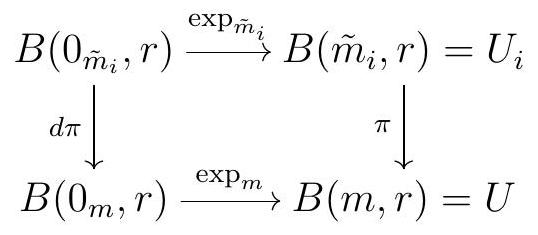
\includegraphics[max width=\textwidth, center]{2025_05_20_3825c151ba0898b77b6eg-083}

Die Abbildung $\exp _{m} \circ d \pi$ ist ein Diffeomorphismus zwischen $B\left(0_{\tilde{m}_{i}}, r\right)$ und $U$ (da $d \pi$ ein Diffeomorphismus zwischen $B\left(0_{\tilde{m}_{i}}, r\right)$ und $B\left(0_{m}, r\right)$ ist und $\exp _{m}: B\left(0_{m}, r\right) \rightarrow U$ ein Diffeomorphismus ist). Da auch $\exp _{\tilde{m}_{i}}: B\left(0_{\tilde{m}_{i}}, r\right) \rightarrow U_{i}$ ein Diffeomorphismus ist (da $\tilde{M}$ geodätisch vollständig ist) folgt, dass

$$
\pi: \exp _{\tilde{m}_{i}}\left(B\left(0_{\tilde{m}_{i}}, r\right)\right) \rightarrow U
$$

ein Diffeomorphismus ist.

Insgesamt folgt, dass $\pi: U_{i} \rightarrow U$ ein Diffeomorphismus ist.\\
Jetzt wird noch $\pi^{-1}(U) \subset \cup_{i} U_{i}$ gezeigt. Sei $\tilde{q} \in \pi^{-1}(U)$ und $q:=$ $\pi(\tilde{q}) \in U$. Sei $\gamma:[0, s] \rightarrow M$ die eindeutige minimale, nach Bogenlänge parametrisierte Geodätische von $q$ nach $m$. Dann ist $s<r$. Sei $v:=$ $\gamma^{\prime}(0) \in T_{q} M$. Sei $\tilde{v} \in T_{\tilde{q}} \tilde{M}$ der eindeutige Vektor mit $d \pi(\tilde{v})=v$. Sei $\tilde{\gamma}$ die Geodätische mit $\tilde{\gamma}(0)=\tilde{q}$ und $\tilde{\gamma}^{\prime}(0)=\tilde{v}$. Da ( $\tilde{M}, \tilde{g}$ ) geodätisch vollständig ist, ist diese Geodätische auf ganz $\mathbb{R}$ definiert.

Andererseits ist $\pi \circ \tilde{\gamma}=\gamma$ und somit $\pi(\tilde{\gamma}(s))=\gamma(s)=m$. Damit ist $\tilde{\gamma}(s)=\tilde{m}_{i}$ für ein $i$ und $\tilde{q} \in B\left(\tilde{m}_{i}, r\right)=U_{i}$.

Zur Erinnerung: eine Mannigfaltigkeit $M$ heisst einfach zusammenhängend, wenn $M$ zusammenhängend ist und jede geschlossene Kurve $\gamma:[0,1] \rightarrow M$ auf einen Punkt kontrahiert werden kann, d.h. es gibt stetige Abbildung $H:[0,1] \times[0,1] \rightarrow M$ so dass $H(s, 0)=$ $\gamma(s), H(s, 1)=p_{0} \in M$ für alle $s$ und $H(0, t)=H(1, t)$ für alle $t$.

Lemma 6.2. Sei $\pi: \tilde{M} \rightarrow M$ eine Überlagerungsabbildung. Ist $\tilde{M}$ zusammenhängend und $M_{\sim}$ einfach zusammenhängend, so ist $\pi$ ein Diffeomorphismus zwischen $\tilde{M}$ und $M$.

Beweis. Jede Kurve $\gamma$ in $M$ kann zu einer Kurve $\tilde{\gamma}$ in $\tilde{M}$ geliftet werden. Ist der Anfangspunkt $\tilde{\gamma}(0) \in \pi^{-1}(\gamma(0))$ vorgegeben, so ist der Lift eindeutig bestimmt.

Angenommen, $\pi$ ist kein Diffeomorphismus. Dann gibt es $p_{0} \in M$, so dass $\pi^{-1}\left(p_{0}\right)$ aus mehreren Punkten besteht. Sei $\tilde{\gamma}:[0,1] \rightarrow \tilde{M}$ eine Kurve, die zwei verschiedene Punkte $q_{0}, q_{1}$ aus $\pi^{-1}\left(p_{0}\right)$ verbindet. Setze $\gamma:=\pi \circ \tilde{\gamma}$. Dann ist $\tilde{\gamma}$ der eindeutige Lift von $\gamma$ mit $\tilde{\gamma}(0)=q_{0}$.

Da $M$ einfach zusammenhängend ist, gibt es eine Homotopie $H$, so dass $H(s, 0)=\gamma(s), H(s, 1)=p_{0}$ und $H(0, t)=H(1, t)=p_{0}$ für alle $s$ und $t$.

Die Kurve $c_{t}:=H(\cdot, t)$ ist eine geschlossene Kurve mit Anfangsund Endpunkt $p_{0}$. Wir liften diese zu einer Kurve $\tilde{c}_{t}$ in $\tilde{M}$ mit $\tilde{c}_{t}(0)=$ $q_{0}$. Da $H$ und das Liften von Kurven stetig sind, ist die Abbildung $t \mapsto \tilde{c}_{t}(1)$ stetig. Aber $\tilde{c}_{t}(1)$ ist in der diskreten Menge $\pi^{-1}\left(p_{0}\right)$ für alle $t$. Also muss $\tilde{c}_{t}(1)$ konstant sein. Jedoch ist $\tilde{c}_{0}(1)=\tilde{\gamma}(1)=q_{1}$, während $\tilde{c}_{1}(1)=q_{0}$ (der Lift einer konstanten Kurve ist wieder eine konstante Kurve).

Theorem 6.3 (Mannigfaltigkeiten konstanter Schnittkrümmung). Sei ( $M, g$ ) eine vollständige, einfach zusammenhängende Riemannsche Mannigfaltigkeit mit konstanter Schnittkrümmung. Dann ist ( $M, g$ ) isometrisch zu $\mathbb{R}^{n}$, falls $K \equiv 0$; zu ( $\mathbb{H}^{n}$, can), falls $K \equiv-1$ und zu ( $S^{n}$, can), falls $K \equiv 1$.

Bemerkung: falls $K \equiv c \neq 0$, so kann man die Krümmung durch Skalieren der Metrik zu $\pm 1$ machen.

Beweis. Sei $m \in M, v \in T_{m} M$ und setze $c(t):=\exp _{m}(t v)$. Seien $u_{1}, u_{2} \in T_{m} M$ und sei $U_{i}$ das parallele Vektorfeld längs $c$ mit $U_{i}(0)=$ $u_{i}, i=1,2$. Sei $Y_{i}$ das Jacobifeld längs $c$ mit $Y_{i}(0)=0, Y_{i}^{\prime}(0)=u_{i}$. Nach Korollar 6.5 gilt

$$
Y_{i}(t)=d_{t v} \exp _{m}\left(t u_{i}\right)
$$

Für $Y$ gilt ausserdem die Jacobigleichung $Y^{\prime \prime}+R\left(c^{\prime}, Y\right) c^{\prime}=0$.\\
(1) Sei $K \equiv 0$, d.h. $R \equiv 0$. Dann ist $Y_{i}^{\prime \prime}(t)=0$, also $Y_{i}(t)=t U_{i}(t)$. Es folgt

$$
\begin{aligned}
\left\langle d_{t v} \exp _{m} t u_{1}, d_{t v} \exp _{m} t u_{2}\right\rangle & =\left\langle Y_{1}(t), Y_{2}(t)\right\rangle \\
& =t^{2}\left\langle U_{1}(t), U_{2}(t)\right\rangle \\
& =\left\langle t u_{1}, t u_{2}\right\rangle
\end{aligned}
$$

Also ist $\exp _{m}: T_{m} M \rightarrow M$ eine lokale Isometrie. Nach Satz 6.1 ist $\exp _{m}: T_{m} M \rightarrow M$ eine Überlagerungsabbildung.

Aus Lemma 6.2 folgt, dass $\exp _{m}$ ein Diffeomorphimus, und damit eine Isometrie ist.\\
(2) Sei $K \equiv-1$. Dann folgt $Y_{i}^{\prime \prime}=Y_{i}$, d.h. $Y_{i}(t)=\sinh (t) U_{i}(t)$. Sei $\tilde{m} \in \mathbb{H}^{n}$ und sei $f: T_{m} M \rightarrow T_{\tilde{m}} \mathbb{H}^{n}$ eine Isometrie (da beides Euklidische Vektorräume gleicher Dimension sind, existiert so eine Isometrie).

Setze $\tilde{u}_{i}:=f\left(u_{i}\right), \tilde{v}:=f(v)$, und seien $\tilde{U}_{i}, \tilde{Y}_{i}$ die entsprechenden parallelen bzw. Jacobifelder längs der Geodätischen $t \mapsto \exp _{\tilde{m}} t \tilde{v}$. Dann gilt auch $\tilde{Y}_{i}(t)=\sinh (t) \tilde{U}_{i}(t)$ (siehe explizite Berechnung der Jacobifelder in Kapitel 6).

Wir wissen, dass $\exp _{\tilde{m}}: T_{\tilde{m}} \mathbb{H}^{n} \rightarrow \mathbb{H}^{n}$ ein Diffeomorphismus ist. Daher können wir eine glatte Abbildung

$$
F:=\exp _{m} \circ f^{-1} \circ \exp _{\tilde{m}}^{-1}: \mathbb{H}^{n} \rightarrow M
$$

definieren. Mit einer Rechnung wie im Fall $K \equiv 0$ ergibt sich, dass $F$ eine lokale Isometrie ist. Der Rest des Beweises ist analog zum Fall $K \equiv 0$.\\
(3) Sei $K \equiv 1$. Dann ist $Y_{i}(t)=\sin (t) U_{i}(t)$. Ist $\tilde{m} \in S^{n}$, so ist $\exp _{\tilde{m}}: B(0, \pi) \subset T_{\tilde{m}} S^{n} \rightarrow S^{n} \backslash\{-\tilde{m}\}$ ein Diffeomorphismus. Also gibt es wie im vorigen Fall eine lokale Isometrie $F$ von\\
$S^{n} \backslash\{-\tilde{m}\}$ nach $M$. Das zugehörige Diagramm ist\\
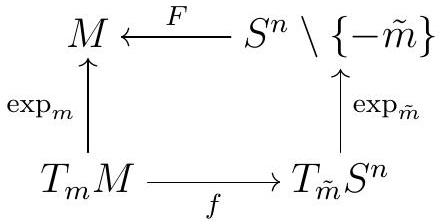
\includegraphics[max width=\textwidth, center]{2025_05_20_3825c151ba0898b77b6eg-086}

Sei $\tilde{m}^{\prime} \neq \pm \tilde{m}$ und setze $m^{\prime}:=F\left(\tilde{m}^{\prime}\right)$. Wir wiederholen die Prozedur mit diesem Punkt. Da $F: S^{n} \backslash\{-\tilde{m}\} \rightarrow M$ eine lokale Isometrie ist, ist

$$
\left.d F\right|_{\tilde{m}^{\prime}}: T_{\tilde{m}^{\prime}} S^{n} \rightarrow T_{m^{\prime}} M
$$

eine Isometrie. Auch die Inverse

$$
\left(\left.d F\right|_{\tilde{m}^{\prime}}\right)^{-1}: T_{m^{\prime}} M \rightarrow T_{\tilde{m}^{\prime}} S^{n}
$$

ist dann eine Isometrie.\\
Dann ist wie eben

$$
F_{1}=\left.\exp _{m^{\prime}} \circ d F\right|_{\tilde{m}^{\prime}} \circ \exp _{\tilde{m}^{\prime}}^{-1}
$$

eine lokale Isometrie $F_{1}: S^{n} \backslash\left\{-\tilde{m}^{\prime}\right\} \rightarrow M$.\\
Es ist $F_{1}\left(\tilde{m}^{\prime}\right)=m^{\prime}=F\left(\tilde{m}^{\prime}\right)$ und $\left.d F_{1}\right|_{\tilde{m}^{\prime}}=\left.\left.d \exp _{m^{\prime}}\right|_{0} \circ d F\right|_{\tilde{m}^{\prime}} \circ\left(\left.\left(d \exp _{\tilde{m}}\right)\right|_{0}\right)^{-1}=\left.d F\right|_{\tilde{m}^{\prime}}$.

Sei $\tilde{c}(t), 0 \leq t<\pi$ eine Geodätische auf $S^{n}$ mit $\tilde{c}(t)=\tilde{m}^{\prime}$, die nicht durch $-\tilde{m}$ geht. Da $F$ und $F_{1}$ lokale Isometrien sind, sind $c(t):=F(\tilde{c}(t))$ und $c_{1}(t):=F_{1}(\tilde{c}(t))$ Geodätische. Es gilt aber $c_{1}(0)=F(\tilde{c}(0))=F\left(\tilde{m}^{\prime}\right)=F_{1}\left(\tilde{m}^{\prime}\right)=c_{1}(0)$ und

$$
c^{\prime}(0)=\left.d F\right|_{\tilde{m}^{\prime}}\left(\tilde{c}^{\prime}(0)\right)=\left.d F_{1}\right|_{\tilde{m}^{\prime}}\left(\tilde{c}^{\prime}(0)\right)=c_{1}^{\prime}(0) .
$$

Es folgt $c=c_{1}$ und somit $F=F_{1}$ auf allen Punkten außerhalb der Geodätischen durch $\tilde{m}$ und $-\tilde{m}^{\prime}$. Da $F$ und $F_{1}$ beide stetig sind, müssen sie dort, wo sie beide definiert sind, übereinstimmen.

Diese beiden Abbildungen können also zu einer lokalen Isometrie zwischen $S^{n}$ und $M$ verklebt werden. Der Rest des Argumentes ist wieder der gleiche.

Bemerkung: ist ( $M, g$ ) nicht einfach zusammenhängend, so gibt es eine einfach zusammenhängende Überlagerung $(\tilde{M}, \tilde{g}) \rightarrow(M, g)$ (die sogenannte universelle Überlagerung), auf welche das Theorem angewendet werden kann. Es kann daher auch wie folgt formuliert werden:

Theorem 6.4. Ist ( $M, g$ ) eine vollständige Riemannsche Mannigfaltigkeit mit konstanter Schnittkrümmung, so ist die universelle Überlagerung $\mathbb{R}^{n}$, falls $K \equiv 0 ; \mathbb{H}^{n}$, falls $K \equiv-1$ und $S^{n}$, falls $K \equiv 1$.

Zum Beispiel hat $\mathbb{R P}^{n}$ Schnittkrümmung $\equiv 1$, und die universelle Überlagerung ist $S^{n}$. Quotienten von $S^{3}$ sind die Linsenräume. Interessanter sind allerdings Quotienten des hyperbolischen Raumes, sogenannte hyperbolische Mannigfaltigkeiten. Diese spielen in vielen Bereichen der Mathematik (unter anderem in der Zahlentheorie) eine grosse Rolle.

\section*{KAPITEL 6}
\section*{Volumen Riemannscher Mannigfaltigkeiten}
\section*{1. Der Schnittort}
Sei $(M, g)$ eine vollständige Riemannsche Mannigfaltigkeit, $m \in M$. Für $v \in T_{m} M$ sei $c_{v}$ die eindeutige Geodätische mit $c_{v}(0)=m, c_{v}^{\prime}(0)=$ $v$. Diese ist auf ganz $\mathbb{R}$ definiert, aber nicht unbedingt minimal. Sei

$$
U_{m}:=\left\{v \in T_{m} M \mid c_{v} \text { ist minimal auf }[0,1+\epsilon] \text { für ein } \epsilon>0\right\} \text {. }
$$

Dann ist $U_{m}$ eine offene Umgebung von $0 \in T_{m} M$ und wir bezeichnen den Rand mit $\partial U_{m}$.

Definition 1.1. Der Schnittort von $m$ ist

$$
\operatorname{Cut}(m):=\exp _{m}\left(\partial U_{m}\right) .
$$

Bemerkung (ohne Beweis): Für $v \in \partial U_{m}$ gibt es (nur) zwei Gründe, die auch simultan auftreten können. Der erste Grund ist, dass es eine weitere minimale Geodätische zwischen $c_{v}(0)$ und $c_{v}(1)$ gibt. Der zweite Grund ist, dass $c_{v}(0)$ und $c_{v}(1)$ konjugiert sind. Dann kann eine Fortsetzung von $c_{v}$ über den Punkt $c_{v}(1)$ hinaus nicht minimal sein nach Theorem 5.4.

Satz 1.2. Die Mannigfaltigkeit $M$ lässt sich disjunkt zerlegen in

$$
M=\exp _{m}\left(U_{m}\right) \cup \operatorname{Cut}(m) .
$$

Beweis. Sei $x \in M$. Dann gibt es eine minimale Geodätische $c_{v}$ von $m$ nach $x$. Ohne Einschränkung sei $c_{v}$ auf $[0,1]$ parametrisiert. Dann ist $v \in \overline{U_{m}}=U_{m} \cup \partial U_{m}$. Es folgt $M=\exp _{m}\left(U_{m}\right) \cup \operatorname{Cut}(m)$.

Angenommen die Vereinigung ist nicht disjunkt. Dann gibt es $x \in$ $\exp _{m}\left(U_{m}\right) \cap \operatorname{Cut}(m)$. Wegen $x \in \exp _{m}\left(U_{m}\right)$ gibt es eine Geodätische $c$ mit $c(0)=m, c(1)=x$, welche auf $[0,1+\epsilon]$ minimal ist. Andererseits impliziert $x \in \operatorname{Cut}(m)$, dass es eine Geodätische $\gamma$ gibt mit $\gamma(0)=$ $m, \gamma(1)=x$, welche minimal auf $[0,1]$, aber nicht darüber hinaus ist.

Dann kann aber auch $c$ nicht minimal über 1 hinaus sein: da $c \neq \gamma$ gilt insbesondere $c^{\prime}(1) \neq \gamma^{\prime}(0)$. Betrachte die Kurve $\tau$ mit $\tau(t)=\gamma(t)$ für $t \in[0,1]$ und $\tau(t)=c(t)$ für $t \in[1,1+\epsilon]$. Dann ist $\tau$ minimal, hat aber bei $t=1$ einen Knick im Widerspruch zu Theorem 3.4.

Beispiel: der Schnittort eines Punktes auf der Sphäre ist der antipodale Punkt. Der Schnittort eines Punktes $m$ des $n$-dimensionalen reell-projektiven Raumes besteht aus den zu $m$ senkrechten Punkten, diese bilden einen ( $n-1$ )-dimensionalen reell-projektiven Raum.

\section*{2. Beispiele für Volumenberechnungen}
Definition 2.1. Eine Dichte auf einer glatten Mannigfaltigkeit M, versehen mit einem Atlas $\left(U_{i}, \phi_{i}\right)$, ist gegeben durch ein Maß $\mu_{i}$ auf $\phi_{i}\left(U_{i}\right)$ mit folgenden Eigenschaften:\\
(1) $\mu_{i}$ ist absolut stetig mit strikt positiver Dichtefunktion bezüglich dem Lebesguemaß;\\
(2) ist $f$ eine stetige Funktion mit kompaktem Träger in $\phi_{i}\left(U_{i} \cap\right.$ $U_{j}$ ), dann gilt

$$
\int_{\phi_{i}\left(U_{i} \cap U_{j}\right)} f d \mu_{i}=\int_{\phi_{j}\left(U_{i} \cap U_{j}\right)}\left(f \circ \phi_{i} \circ \phi_{j}^{-1}\right)\left|J\left(\phi_{i} \circ \phi_{j}^{-1}\right)\right| d \mu_{j}
$$

Hier ist $J$ die Jacobideterminante.\\
Jede Volumenform (d.h. nirgends verschwindende $n$-Form) definiert eine Dichte auf $M$.

Ist eine Dichte auf $M$ gegeben, so hat man ein Maß wie folgt. Ist $f$ eine stetige Funktion auf $M$ mit Träger in $U_{i}$, so setzt man

$$
\int_{M} f d \delta:=\int_{\phi_{i}\left(U_{i}\right)} f \circ \phi_{i}^{-1} d \mu_{i}
$$

Der allgemeine Fall wird über eine Zerlegung der Eins auf diesen zurückgeführt. Dann ist alles wohldefiniert.

Sind $\delta, \delta^{\prime}$ zwei Dichten auf $M$, so gibt es eine stetige Funktion $f$ mit $\delta^{\prime}=f \delta$.

Definition 2.2. Eine Teilmenge $A \subset M$ hat Maß 0 (oder ist eine Nullmenge), wenn $\delta(A)=0$ für eine (und dann für jede) Dichte $\delta$ auf M.

Sei nun ( $M, g$ ) eine vollständige Riemannsche Mannigfaltigkeit. In jeder Karte ( $U_{i}, \phi_{i}$ ) definieren wir

$$
\mu_{i}:=\sqrt{\operatorname{det}\left(g_{i j}\right)} d x_{1} \ldots d x_{n}
$$

Diese Familie erfüllt die Bedingungen einer Dichte auf $M$. Hierzu benutzt man einen Variablenwechsel auf $\mathbb{R}^{n}$, der Faktor $\sqrt{\operatorname{det}\left(g_{i j}\right)}$ ist genau so gewählt, dass diese Unabhängigkeit gilt.

Definition 2.3. Die so definierte Dichte ist die kanonische Volumendichte auf $(M, g)$ und wird mit $v_{g}$ bezeichnet.

Das Volumen von ( $M, g$ ) ist definiert als $\int_{M} v_{g}$ und kann endlich oder unendlich sein.

Sei zum Beispiel $g=d r^{2}+f^{2}(r) d \theta^{2}$ eine Metrik auf $\mathbb{R}^{2}$, ausgedrückt in Polarkoordinaten. Dann ist

$$
\operatorname{vol}\left(\mathbb{R}^{2}, g\right)=2 \pi \int_{0}^{\infty} f(r) d r
$$

Lemma 2.4. Für jedes $m \in M$ ist der Schnittort Cut $(m)$ eine Nullmenge.

Beweis. Es ist $\operatorname{Cut}(m)=\exp _{m}\left(\partial U_{m}\right)$. Da $\partial U_{m}$ eine Nullmenge in $T_{m} M$ ist und $\exp _{m}$ stetig ist, folgt die Behauptung.

Allgemeiner können wir das Volumen von einem Punkt aus wie folgt berechnen. Aus dem Theorem von Hopf-Rinow folgt, dass jeder Punkt von $M$ mit einem festen Punkt $m$ durch eine minimale Geodätische verbunden werden kann. Außerhalb des Schnittortes ist diese Geodätische sogar eindeutig. Der Schnittort hat Volumen 0, also gilt

$$
\operatorname{vol}(M, g)=\int_{U_{m}} \exp _{m}^{*} v_{g}
$$

Das kann wie folgt umgeformt werden. Sei $c(t)=\exp _{m}(t u)$ eine Geodätische und $\left\{u, e_{2}, \ldots, e_{n}\right\}$ eine Orthonormalbasis von $T_{m} M$. Betrachte Jacobifelder $Y_{i}$ längs $c$ mit $Y_{i}(0)=0, Y_{i}^{\prime}(0)=e_{i}$. Aus Korollar 6.5 folgt $\left.\left(d \exp _{m}\right)\right|_{t u} u=c^{\prime}(t)$ und $\left(d \exp _{m}\right)_{t u} e_{i}=\frac{1}{t} Y_{i}(t)$. Wir setzen

$$
J(u, t):=t^{-(n-1)} \sqrt{\operatorname{det}\left(g\left(Y_{i}(t), Y_{j}(t)\right)\right.}
$$

Dann gilt $\exp _{m}^{*} v_{g}=J(u, t) d x_{1} \ldots d x_{n}=J(u, t) t^{n-1} d t d u$, wobei $d u$ das kanonische Maß auf der Einheitssphäre in $T_{m} M$ bezeichnet. Ist $\rho(u)$ der Abstand zum Schnittort in Richtung $u$ (eventuell kann er unendlich sein), so folgt


\begin{equation*}
\operatorname{vol}(M, g)=\int_{S^{n-1}} \int_{0}^{\rho(u)} J(u, t) t^{n-1} d t d u \tag{11}
\end{equation*}


Man beachte, dass $\lim _{t \rightarrow 0} J(u, t)=1$ für alle $u$. Beispiele:\\
(1) Für die Sphäre $S^{n}$ mit der kanonischen Metrik gilt $Y_{i}(t)=$ $\sin (t) E_{i}(t)$ mit $E_{i}$ parallelen Vektorfeldern, $\rho(u)=\pi$ und somit

$$
\begin{aligned}
\operatorname{vol}\left(S^{n}, c a n\right) & =\int_{S^{n-1}} \int_{0}^{\pi}\left(\frac{\sin t}{t}\right)^{n-1} t^{n-1} d u d t \\
& =\operatorname{vol}\left(S^{n-1}, c a n\right) \int_{0}^{\pi} \sin ^{n-1}(t) d t
\end{aligned}
$$

Induktiv kann man zeigen, dass

$$
\operatorname{vol}\left(S^{2 m}, c a n\right)=\frac{2(4 \pi)^{m} m!}{(2 m)!}, \quad \operatorname{vol}\left(S^{2 m+1}, c a n\right)=\frac{2 \pi^{m+1}}{m!}
$$

(2) Das Volumen des hyperbolischen Raumes ist unendlich. Für $R>0$ ergibt sich wie für die Sphäre

$$
\operatorname{vol}\left(B_{m}(R)\right)=\operatorname{vol}\left(S^{n-1}, \text { can }\right) \int_{0}^{R} \sinh ^{n-1}(r) d r
$$

Dieser Ausdruck wächst exponentiell schnell (von der Ordnung $\exp ((n-1) R))$.\\
(3) Für den komplex-projektiven Raum wähle eine orthonormale Basis $\left\{u, e_{2}, \ldots\right\}$ von $T_{m} \mathbb{C}^{n}$ mit $e_{2}=J u$. Dann sind nach (9) und (10) die Jacobifelder gegeben durch

$$
\begin{aligned}
& Y_{2}(t)=\sin (t) \cos (t) E_{2}(t) \\
& Y_{i}(t)=\sin (t) E_{i}(t), i \geq 3
\end{aligned}
$$

Der Abstand vom Schnittort ist $\frac{\pi}{2}$ und es ergibt sich

$$
\operatorname{vol}\left(\mathbb{C P}^{n}, c a n\right)=\int_{S^{2 n-1}} \int_{0}^{\frac{\pi}{2}} \sin ^{2 n-1} t \cos t d u d t=\frac{\pi^{n}}{n!}
$$

\section*{3. Volumen und Krümmung}
Lemma 3.1. Sei $A(t)$ eine glatte Kurve von $n \times n$-Matrizen mit $A(0)=$ Id. Dann gilt

$$
\left.\frac{d}{d t}\right|_{t=0} \operatorname{det} A(t)=\operatorname{tr} A^{\prime}(0)
$$

Beweis. Per Induktion über $n$. Ist $n=1$, so ist die Aussage trivial. Für $n>1$ entwickeln wir $\operatorname{det} A$ nach der ersten Zeile und bekommen

$$
\operatorname{det} A(t)=\sum_{i=1}^{n}(-1)^{i+1} a_{1 i}(t) \operatorname{det} A_{i}(t)
$$

wobei $A_{i}(t)$ die Matrix ist, die aus $A(t)$ durch Streichen der ersten Zeile und $i$-ten Spalte entsteht. Es folgt

$$
\begin{aligned}
\left.\frac{d}{d t}\right|_{t=0} \operatorname{det} A(t)= & a_{11}^{\prime}(0) \underbrace{\operatorname{det} A_{1}(0)}_{=1}+\underbrace{a_{11}(0)}_{=1} \underbrace{\left(\operatorname{det} A_{1}(0)\right)^{\prime}}_{=\operatorname{tr} A_{1}^{\prime}(0)}+ \\
& \sum_{i=2}^{n} a_{1 i}^{\prime}(0) \underbrace{\operatorname{det} A_{i}(0)}_{=0}+\underbrace{a_{1 i}(0)}_{=0}\left(\operatorname{det} A_{i}(0)\right)^{\prime} \\
= & a_{11}^{\prime}(0)+\operatorname{tr} A_{1}^{\prime}(0)=\operatorname{tr} A^{\prime}(0)
\end{aligned}
$$

Lemma 3.2. Sei $\phi$ eine symmetrische Bilinearform auf $\mathbb{R}^{n}$. Dann gilt

$$
\int_{S^{n-1}} \phi(v, v) d v=\frac{1}{n} \operatorname{vol}\left(S^{n-1}\right) \operatorname{tr}(\phi)
$$

Beweis. Seien $v_{1}, \ldots, v_{n}$ die Koordinaten von $v$. Dann ist $\phi(v, v)=$ $\sum_{i, j} v_{i} v_{j} \phi\left(e_{i}, e_{j}\right)$, also

$$
\int_{S^{n-1}} \phi(v, v) d v=\sum_{i, j} \phi\left(e_{i}, e_{j}\right) \int_{S^{n-1}} v_{i} v_{j} d v
$$

Für $i \neq j$ verschwindet das Integral aus Symmetriegründen. Für $i=j$ ist es (ebenfalls wegen Symmetrie) unabhängig von $i$. Da $\sum_{i} v_{i}^{2}=1$, ist dieses Integral genau $\frac{1}{n} \operatorname{vol}\left(S^{n-1}\right)$ und die Behauptung des Lemmas folgt.

Theorem 3.3 (Volumen kleiner Bälle). Seim ein Punkt von $(M, g)$. Dann gilt

$$
\operatorname{vol} B_{m}(r)=r^{n} \operatorname{vol}\left(B^{n}\right)\left(1-\frac{s}{6(n+2)} r^{2}+o\left(r^{2}\right)\right),
$$

wobei $s$ die Skalarkrümmung in $m$ ist, $n$ die Dimension von $M$ und $r \rightarrow 0$.

In erster und zweiter Ordnung ist das Volumen also wie im Euklidschen Fall, und der nächste Term wird durch die Skalarkrümmung festgelegt. Insbesondere ist das Vorzeichen von $s$ dafür ausschlaggebend, ob kleine Bälle in ( $M, g$ ) kleineres oder größeres Volumen als im Euklidschen Raum haben.

Beweis. Für $r$ kleiner als der Abstand zum Schnittort gilt

$$
\operatorname{vol} B_{m}(r)=\int_{S^{n-1}} \int_{0}^{r} J(u, t) t^{n-1} d t d u
$$

Wähle eine Geodätische $c$ mit $c(0)=m, c^{\prime}(0)=u$ und $Y_{i}$ Jacobifelder $\operatorname{mit} Y_{i}(0)=0, Y_{i}^{\prime}(0)=e_{i}$, wobei wieder $\left\{u, e_{2}, \ldots, e_{n}\right\}$ eine Orthonormalbasis von $T_{m} M$ ist. Die Jacobigleichung liefert

$$
Y_{i}^{\prime \prime}(s)+R\left(c^{\prime}(s), Y_{i}(s)\right) c^{\prime}(s)=0
$$

Insbesondere ist $Y_{i}(0)=0, Y_{i}^{\prime}(0)=e_{i}, Y_{i}^{\prime \prime}(0)=0$. Wir benötigen einen weiteren Term. Dazu leiten wir die Jacobigleichung nach $s$ ab und setzen $s=0$. Da $Y_{i}(0)=0$ spielt dabei nur der Term eine Rolle, bei dem\\
$Y_{i}(s)$ abgeleitet wird (bei den anderen Termen wird entweder $R$ oder $c^{\prime}(s)$ abgeleitet). Es folgt

$$
Y_{i}^{\prime \prime \prime}(0)=-R\left(c^{\prime}(0), Y_{i}^{\prime}(0)\right) c^{\prime}(0)=-R\left(u, e_{i}\right) u=-\sum_{j} R\left(u, e_{i}, u, e_{j}\right) e_{j}
$$

Aus Lemma 4.1 ergibt sich

$$
Y_{i}(t)=t E_{i}(t)-\sum_{j} \frac{t^{3}}{6} R\left(u, e_{i}, u, e_{j}\right) E_{j}(t)+o\left(t^{3}\right)
$$

Es folgt $g\left(Y_{i}(t), Y_{j}(t)\right)=t^{2} \delta_{i j}-\frac{t^{4}}{3} R\left(u, e_{i}, u, e_{j}\right)+o\left(t^{4}\right)$. Lemma 3.1 impliziert

$$
\operatorname{det}\left(g\left(Y_{i}(t), Y_{j}(t)\right)\right)=t^{2(n-1)}\left(1-\frac{t^{2}}{3} \operatorname{Ric}(u, u)+o\left(t^{2}\right)\right)
$$

und somit

$$
J(u, t)=t^{-(n-1)} \sqrt{\operatorname{det}\left(g\left(Y_{i}(t), Y_{j}(t)\right)\right)}=1-\frac{t^{2}}{6} \operatorname{Ric}(u, u)+o\left(t^{2}\right)
$$

Einsetzen liefert

$$
\begin{aligned}
\operatorname{vol} B_{m}(r) & =\int_{S^{n-1}} \int_{0}^{r} t^{n-1}\left(1-\frac{t^{2}}{6} \operatorname{Ric}(u, u)+o\left(t^{2}\right)\right) d t d u \\
& =\int_{S^{n-1}}\left(\frac{r^{n}}{n}-\frac{r^{n+2}}{6(n+2)} \operatorname{Ric}(u, u)+o\left(r^{n+2}\right)\right) d u \\
& =\operatorname{vol}\left(S^{n-1}\right) \frac{r^{n}}{n}-\frac{r^{n+2}}{6(n+2)} \frac{\operatorname{vol}\left(S^{n-1}\right)}{n} \operatorname{tr} \operatorname{Ric}+o\left(r^{n+2}\right) \\
& =\frac{r^{n} \operatorname{vol}\left(S^{n-1}\right)}{n}\left(1-\frac{r^{2}}{6(n+2)} s(m)+o\left(r^{2}\right)\right)
\end{aligned}
$$

Der Vorfaktor ist genau das Volumen eines Euklidschen Balles mit Radius $r$.

Mit $V^{a}(r)$ bezeichnen wir das Volumen eines $r$-Balles in der vollständigen, einfach zusammenhängenden Mannigfaltigkeit mit konstanter Schnittkrümmung $a$.

Theorem 3.4 (Bishop-Gunther). Sei ( $M, g$ ) eine vollständige Riemannsche Mannigfaltigkeit und $B_{m}(r)$ ein Ball, der den Schnittort von $m$ nicht trifft.\\
(1) Ist Ric $\geq(n-1)$ ag für eine Konstante $a \in \mathbb{R}$, dann gilt

$$
\operatorname{vol}\left(B_{m}(r)\right) \leq V^{a}(r)
$$

(2) Ist $K \leq b$ für eine Konstante $b \in \mathbb{R}$, dann gilt

$$
\operatorname{vol}\left(B_{m}(r)\right) \geq V^{b}(r)
$$

Beweis. (1) Zunächst eine Vorbemerkung. Sei $c$ eine nach Bogenlänge parametrisierte Geodätische und $Y_{i}, i=2, \ldots, n$ Jacobifelder längs $c$ mit $Y_{i}(0)=0$, so dass $c^{\prime}(0), Y_{2}^{\prime}(0), \ldots, Y_{n}^{\prime}(0)$ eine Basis (aber nicht unbedingt Orthonormalbasis) von $T_{m} M$ bilden.

Seien $\tilde{Y}_{2}, \ldots, \tilde{Y}_{n}$ Jacobifelder längs $c$ mit $\tilde{Y}_{i}(0)=0, \tilde{Y}_{i}^{\prime}(0)=$ $e_{i}$, mit Orthonormalbasis $c^{\prime}(0), e_{2}, \ldots, e_{n}$. Dann gibt es eine invertierbare reelle $(n-1) \times(n-1)$-Matrix $C$ mit $Y_{i}=\sum_{j} C_{i j} \tilde{Y}_{j}$. Es folgt $\operatorname{det} g\left(Y_{i}^{\prime}(0), Y_{j}^{\prime}(0)\right)=\operatorname{det} C^{2} \operatorname{det} g\left(\tilde{Y}_{i}^{\prime}(0), \tilde{Y}_{j}^{\prime}(0)\right)=\operatorname{det} C^{2}$ und $\operatorname{det} g\left(Y_{i}(t), Y_{j}(t)\right)=\operatorname{det} C^{2} \operatorname{det} g\left(\tilde{Y}_{i}(t), \tilde{Y}_{j}(t)\right)$.

Somit erhalten wir

$$
\begin{aligned}
J(u, t) & =t^{-(n-1)} \sqrt{\operatorname{det} g\left(\tilde{Y}_{i}(t), \tilde{Y}_{j}(t)\right)} \\
& =t^{-(n-1)} \frac{\sqrt{\operatorname{det} g\left(Y_{i}(t), Y_{j}(t)\right)}}{\sqrt{\operatorname{det} g\left(Y_{i}^{\prime}(0), Y_{j}^{\prime}(0)\right)}}
\end{aligned}
$$

(2) Wähle eine Orthonormalbasis $\left\{u, e_{2}, \ldots, e_{n}\right\}$ von $T_{m} M$ und setze $c(t):=\exp _{m}(t u)$. Seien $E_{i}$ die parallelen Vektorfelder längs $c$ mit $E_{i}(0)=e_{i}$, wobei $2 \leq i \leq n$.

Fixiere $0<r<\rho(u)$, wobei $\rho(u) \in(0, \infty]$ die Länge von $c$ von $m$ bis zum Schnittort ist. Dann gibt es ein eindeutiges Jacobifeld $Y_{i}^{r}$ mit

$$
Y_{i}^{r}(0)=0, Y_{i}^{r}(r)=E_{i}(r)
$$

Die Existenz sieht man wie folgt: da $\left(d \exp _{m}\right)_{t u}: T_{m} M \rightarrow$ $T_{c(t)} M$ ein Isomorphismus ist, gibt es einen Vektor $v \in T_{m} M$ mit $\left(d \exp _{m}\right)_{t u}(r v)=E_{i}(r)$. Dann ist

$$
Y_{i}^{r}(t)=\left(d \exp _{m}\right)_{t u}(t v)
$$

als Variationsfeld einer geodätischen Variation ein Jacobifeld und hat die gewünschten Eigenschaften.

Nach der Vorbemerkung gilt

$$
J(u, t)=t^{-(n-1)} \frac{\sqrt{\operatorname{det} g\left(Y_{i}(t), Y_{j}(t)\right)}}{\sqrt{\operatorname{det} g\left(Y_{i}^{\prime}(0), Y_{j}^{\prime}(0)\right)}}
$$

Wir setzen

$$
D(t):=\operatorname{det} g\left(Y_{i}(t), Y_{j}(t)\right)
$$

und

$$
f(t):=J(u, t)
$$

(3) Sei\\
$I(X, Y)=\int_{0}^{r}\left[\left\langle X^{\prime}(s), Y^{\prime}(s)\right\rangle-R\left(X(s), c^{\prime}(s), Y(s), c^{\prime}(s)\right)\right] d s$.\\
Sind $X, Y$ Vektorfelder längs $c$, welche an den Endpunkten verschwinden, so ist das die Indexform. Im Allgemeinen ist es eine quadratische Form. Wir behaupten, dass


\begin{equation*}
\frac{f^{\prime}(r)}{f(r)}=\sum_{i=2}^{n} I\left(Y_{i}^{r}, Y_{i}^{r}\right)-\frac{n-1}{r} \tag{12}
\end{equation*}


Ableiten der Gleichung $f(t)=t^{-(n-1)} C \sqrt{D(t)}$ liefert

$$
\frac{f^{\prime}(t)}{f(t)}=\frac{D^{\prime}(t)}{2 D(t)}-\frac{n-1}{t}
$$

Für den Fall $t=r$ ist die Matrix $g\left(Y_{i}^{r}, Y_{j}^{r}\right)$ die Identitätsmatrix und es folgt mit Lemma 3.1

$$
D^{\prime}(r)=2 \sum_{i=2}^{n} g\left(\left(Y_{i}^{r}\right)^{\prime}(r), Y_{i}^{r}(r)\right)
$$

Andererseits gilt für ein Jacobifeld

$$
\begin{aligned}
I(Y, Y) & =\int_{0}^{r}\left(\left|Y^{\prime}(s)\right|^{2}-R\left(Y(s), c^{\prime}(s), Y(s), c^{\prime}(s)\right)\right) d s=\left.g\left(Y, Y^{\prime}\right)\right|_{0} ^{r} \\
& =\int_{0}^{r}\left(\left|Y^{\prime}(s)\right|^{2}-\left\langle R\left(c^{\prime}(s), Y(s)\right) c^{\prime}(s), Y(s)\right\rangle\right) d s=\left.g\left(Y, Y^{\prime}\right)\right|_{0} ^{r} \\
& =\int_{0}^{r}\left(\left|Y^{\prime}(s)\right|^{2}+\left\langle Y^{\prime \prime}(s), Y(s)\right\rangle\right) d s=\left.g\left(Y, Y^{\prime}\right)\right|_{0} ^{r}
\end{aligned}
$$

Daraus folgt die Behauptung.\\
(4) Sei allgemein $c:[a, b] \rightarrow M$ eine minimale Geodätische, $Y$ ein Jacobifeld längs $c$ und $X$ ein Vektorfeld längs $c$ mit $X(a)=$ $Y(a), X(b)=Y(b)$. Dann ist $I(X-Y, X-Y) \geq 0$, da $c$ minimal ist und $X-Y$ an den Endpunkten verschwindet.

Mit einer analogen Rechnung wie oben gilt

$$
\left.I(X, Y)=\mid g\left(X, Y^{\prime}\right)\right]_{a}^{b}
$$

Da $X$ und $Y$ in den Endpunkten übereinstimmen, gilt

$$
I(Y, Y)=\left[g\left(Y^{\prime}, Y\right)\right]_{a}^{b}=\left[g\left(Y^{\prime}, X\right)\right]_{a}^{b}=I(X, Y)
$$

Es folgt $0 \leq I(X-Y, X-Y)=I(X, X)+I(Y, Y)-2 I(X, Y)=$ $I(X, X)-I(Y, Y)$.\\
(5) Wir setzen

$$
s(t):= \begin{cases}\sin \sqrt{a} t & a>0 \\ t & a=0 \\ \sinh \sqrt{-a} t & a<0\end{cases}
$$

und definieren Vektorfelder

$$
X_{i}^{r}(t):=\frac{s(t)}{s(r)} E_{i}(t)
$$

Die Vorfaktoren sind genau so gewählt, dass auf den Modellmannigfaltigkeiten mit konstanter Schnittkrümmung $a$ sich Jacobifelder ergeben (d.h. $X_{i}^{r}=Y_{i}^{r}$ in diesem Fall). Für unsere Mannigfaltigkeit $M$ sind die $X_{i}^{r}$ natürlich nicht notwendigerweise Jacobifelder, aber wir können mit den obigen Rechnungen die Indizes abschätzen.

Da $X_{i}^{r}$ und $Y_{i}^{r}$ an den Stellen 0 und $r$ übereinstimmen und $c$ minimal ist, folgt nach dem eben Bewiesenen

$$
\sum_{i=2}^{n} I\left(Y_{i}^{r}, Y_{i}^{r}\right) \leq \sum_{i=2}^{n} I\left(X_{i}^{r}, X_{i}^{r}\right)
$$

Mit partieller Integration finden wir

$$
\begin{aligned}
I\left(X_{i}^{r}, X_{i}^{r}\right) & =\int_{0}^{r}\left[\left\langle\left(X_{i}^{r}\right)^{\prime},\left(X_{i}^{r}\right)^{\prime}\right\rangle-R\left(X_{i}^{r}, c^{\prime}, X_{i}^{r}, c^{\prime}\right)\right] d t \\
& =\int_{0}^{r}\left[-\left\langle X_{i}^{r},\left(X_{i}^{r}\right)^{\prime \prime}\right\rangle-R\left(X_{i}^{r}, c^{\prime}, X_{i}^{r}, c^{\prime}\right)\right] d t+\left[\left\langle X_{i}^{r},\left(X_{i}^{r}\right)^{\prime}\right\rangle\right]_{0}^{r} \\
& =\int_{0}^{r}\left[a\left(\frac{s(t)}{s(r)}\right)^{2}-\left(\frac{s(t)}{s(r)}\right)^{2} R\left(E_{i}, c^{\prime}, E_{i}, c^{\prime}\right)\right] d t+\frac{s^{\prime}(r)}{s(r)}
\end{aligned}
$$

Aufsummieren liefert

$$
\sum_{i=2}^{n} I\left(X_{i}^{r}, X_{i}^{r}\right)=\int_{0}^{r}\left(\frac{s(t)}{s(r)}\right)^{2}\left((n-1) a-\operatorname{Ric}\left(c^{\prime}, c^{\prime}\right)\right) d t+(n-1) \frac{s^{\prime}(r)}{s(r)}
$$

Nach Voraussetzung an die Riccikrümmung ist das Integral negativ.

Aus (12) folgt

$$
\begin{aligned}
\frac{f^{\prime}(r)}{f(r)} & =\sum_{i} I\left(Y_{i}^{r}, Y_{i}^{r}\right)-\frac{n-1}{r} \\
& \leq \sum_{i} I\left(X_{i}^{r}, X_{i}^{r}\right)-\frac{n-1}{r} \\
& \leq(n-1) \frac{s^{\prime}(r)}{s(r)}-\frac{n-1}{r} \\
& =(n-1)\left(\frac{s^{\prime}(r)}{s(r)}-\frac{1}{r}\right) \\
& = \begin{cases}(n-1)\left(\sqrt{a} \cot \sqrt{a} r-\frac{1}{r}\right) & a>0 \\
0 & a=0 \\
(n-1)\left(\sqrt{-a} \operatorname{coth} \sqrt{-a} r-\frac{1}{r}\right) & a<0\end{cases}
\end{aligned}
$$

(6) Für die Modellräume gilt überall Gleichheit, also folgt

$$
\frac{f^{\prime}(r)}{f(r)} \leq \frac{f_{a}^{\prime}(r)}{f_{a}(r)}
$$

Es ist $\lim _{t \rightarrow 0} f(t)=\lim _{t \rightarrow 0} J(u, t)=1=\lim _{t \rightarrow 0} f_{a}(t)$.\\
Diese Ungleichung gilt für alle $0<r<\rho(u)$. Es folgt für alle $0<s<\rho(u)$\\
$\log f(s)=\left.\log f(r)\right|_{0} ^{s}=\int_{0}^{s} \frac{f^{\prime}(r)}{f(r)} d r \leq \int_{0}^{s} \frac{f_{a}^{\prime}(r)}{f_{a}(r)} d r=\left.\log f_{a}(r)\right|_{0} ^{s}=\log f_{a}(s)$, also $f(s) \leq f_{a}(s)$.

Aus (11) folgt die erste Behauptung des Theorems.\\
(7) Für den zweiten Teil sei $K \leq b$. Sei $Y$ eines der Jacobifelder $Y_{i}^{r}$. Dann ist\\
$g\left(Y(r), Y^{\prime}(r)\right)=\int_{0}^{r}\left(g\left(Y^{\prime}, Y^{\prime}\right)-R\left(Y, c^{\prime}, Y, c^{\prime}\right)\right) d s \geq \int_{0}^{r}\left(g\left(Y^{\prime}, Y^{\prime}\right)-b g(Y, Y)\right) d s$.\\
Wir schreiben $Y(t)=\sum_{i=2}^{n} y_{i}(t) E_{i}(t)$. Auf der einfach zusammenhängenden Mannigfaltigkeit $M_{b}$ mit konstanter Schnittkrümmung $b$ setze $\tilde{Y}(t)=\sum_{i} y_{i}(t) \tilde{E}_{i}(t)$, wobei $\tilde{c}$ eine Geodätische der Länge $r$ und $\tilde{E}_{i}$ parallele Vektorfelder längs $\tilde{c}$, die zusammen mit $\tilde{c}^{\prime}$ in jedem Punkt eine Orthonormalbasis bilden.

Dann gilt

$$
\left.I(\tilde{Y}, \tilde{Y})=\int_{0}^{r} g\left(\tilde{Y}^{\prime}, \tilde{Y}^{\prime}\right)-b g(\tilde{Y}, \tilde{Y})\right) d t=\int_{0}^{r}\left(g\left(Y^{\prime}, Y^{\prime}\right)-b g(Y, Y)\right) d t
$$

Sei $\tilde{X}_{i}^{r}(t)=\frac{s(t)}{s(r)} \tilde{E}_{i}(t)$. Das ist ein Jacobifeld längs $\tilde{c}$, welches an den Enden von $\tilde{c}$ die gleichen Werte wie $\tilde{Y}_{i}^{r}$ annimmt. Wie oben gilt

$$
I\left(\tilde{Y}_{i}^{r}, \tilde{Y}_{i}^{r}\right) \geq I\left(\tilde{X}_{i}^{r}, \tilde{X}_{i}^{r}\right)
$$

Aus (12), angewendet auf $M$ und $M_{b}$, folgt

$$
\begin{aligned}
\frac{f^{\prime}(r)}{f(r)} & =\sum_{i=2}^{n} I\left(Y_{i}^{r}, Y_{i}^{r}\right)-\frac{n-1}{r} \\
& =\sum_{i=2}^{n} I\left(\tilde{Y}_{i}^{r}, \tilde{Y}_{i}^{r}\right)-\frac{n-1}{r} \\
& \geq \sum_{i=2}^{n} I\left(\tilde{X}_{i}^{r}, \tilde{X}_{i}^{r}\right)-\frac{n-1}{r} \\
& =\frac{f_{b}^{\prime}(r)}{f_{b}(r)}
\end{aligned}
$$

Integrieren liefert $f(s) \geq f_{b}(s)$ und aus (11) folgt vol $B_{m}(r) \geq$ $V^{b}(r)$.

\section*{4. Krümmung und Wachstum der Fundamentalgruppe}
Eine Gruppe $\Gamma$ heisst endlich erzeugt, wenn es endlich viele Elemente $a_{1}, \ldots, a_{k}$ gibt, so das sich jedes Element $g \in \Gamma$ schreiben lässt als Produkt von solchen Generatoren, d.h.

$$
g=\prod_{i} a_{k_{i}}^{r_{i}}, r_{i} \in \mathbb{Z}
$$

Die Zahl $l_{S}(g)=\sum_{i}\left|r_{i}\right|$ heisst Länge von $g$. Diese hängt nicht nur von $g$, sondern von der Wahl der Menge $S$ der Generatoren ab. Mit $\phi_{S}(s)$ wird die Anzahl der Elemente von $\Gamma$ mit Länge kleiner gleich $s$ bezeichnet.

DEFINITION 4.1. (1) Eine endlich erzeugte Gruppe hat exponentielles Wachstum, wenn es $a>0$ gibt mit $\phi_{S}(s) \geq \exp (a s)$ für alle $s$.\\
(2) Eine endlich erzeugte Gruppe hat polynomielles Wachstum vom Grad $\leq n$, wenn es $a>0$ gibt mit $\phi_{S}(s) \leq a s^{n}$ für alle $s$.\\
(3) Eine endlich erzeugte Gruppe hat polynomielles Wachstum vom Grad $n$, falls es polynomiales Wachstum vom Grad $\leq n$ hat, aber nicht vom Grad $\leq(n-1)$.

Ist $\widetilde{S}$ ein anderes Erzeugendensystem, so können wir jeden Erzeuger $\tilde{g} \in \tilde{S}$ als Wort in $S$ schreiben. Ist $C:=\max _{\tilde{g} \in \tilde{S}} l_{S}(\tilde{g})$, so folgt $l_{S} \leq C l_{\tilde{S}}$. Umgekehrt gilt $l_{\tilde{S}} \leq \tilde{C} l_{S}$ mit $\tilde{C}=\max g \in S l_{\tilde{S}}(g)$. Aus diesen beiden Ungleichungen folgt, dass die Bedingungen „exponentielles Wachstum" und „polynomielles Wachstum vom Grad $\leq n$ " unabhängig von der Wahl des Erzeugendensystems sind.

Theorem 4.2 (Milnor-Wolf). Sei ( $M, g$ ) eine vollständige Riemannsche Mannigfaltigkeit mit nichtnegativer Riccikrümmung. Dann hat jede endlich erzeugte Untergruppe $\Gamma$ von $\pi_{1}(M)$ polynomielles Wachstum vom Grad $\leq n$.

Bemerkung: ist $M$ kompakt, so ist $\pi_{1}(M)$ bereits endlich erzeugt.\\
Beweis. Sei ( $\tilde{M}, \tilde{g}$ ) die universelle Riemannsche Überlagerung und $a \in \tilde{M}$. Die Fundamentalgruppe $\pi_{1}(M)$ operiert auf $\tilde{M}$.

Es gibt $r>0$, so dass die Bälle $B(\gamma(a), r)$ alle paarweise disjunkt sind. Sei $S$ ein endliches Erzeugendensystem einer Untergruppe $\Gamma$ von $\pi_{1}(M)$. Ohne Einschränkung sei mit $\gamma \in S$ auch $\gamma^{-1} \in S$.

Setze

$$
L:=\max d\left(a, \gamma_{i}(a)\right), \gamma_{i} \in S
$$

Behauptung: Es gilt für alle $\gamma \in \Gamma$ die Ungleichung $d(a, \gamma(a)) \leq$ $l_{S}(\gamma) L$. Das folgt aus der Definition von $L$ falls $l_{S}(\gamma)=1$. Anderenfalls können wir $\gamma=\gamma^{\prime} \gamma_{i}$ mit $\gamma_{i} \in S, l_{S}\left(\gamma^{\prime}\right)=l(\gamma)-1$ schreiben. Nach Dreiecksungleichung, Induktionsvoraussetzung und der Tatsache, dass $\pi_{1}(M)$ durch Isometrien auf $\tilde{M}$ operiert, gilt dann

$$
\begin{aligned}
d(a, \gamma(a)) & \leq d\left(a, \gamma^{\prime}(a)\right)+d\left(\gamma^{\prime}(a), \gamma^{\prime} \gamma_{i}(a)\right) \\
& =d\left(a, \gamma^{\prime}(a)\right)+d\left(a, \gamma_{i}(a)\right) \\
& \leq l_{S}\left(\gamma^{\prime}\right) L+L=l_{S}(\gamma) L
\end{aligned}
$$

Nimmt man alle solchen $\gamma$, so ergeben sich $\phi_{S}(s)$ paarweise disjunkte Bälle $B(\gamma(a), r)$. Diese gehen durch Elemente der Gruppe isometrisch ineinander über, haben also alle das gleiche Volumen. Für einen Punkt $x \in B(\gamma(a), r)$ ist nach Dreiecksungleichung $d(x, a) \leq$ $d(x, \gamma(a))+d(\gamma(a), a) \leq r+L s$. Mit anderen Worten gilt

$$
B(\gamma(a), r) \subset B(a, L s+r)
$$

Vergleich der Volumina liefert somit

$$
\phi_{S}(s) \operatorname{vol} B(a, r) \leq \operatorname{vol} B(a, L s+r)
$$

Nach Theorem 3.4 gilt aber vol $B(a, L s+r) \leq \operatorname{vol}\left(B_{n}^{\text {eukl }}(1)\right)(L s+$ $r)^{n}$. Also ist

$$
\phi_{S}(s) \leq C_{M}(L s+r)^{n}
$$ und die Behauptung folgt.


\end{document}